%&preformat-disser
\RequirePackage[l2tabu,orthodox]{nag} % Раскомментировав, можно в логе получать рекомендации относительно правильного использования пакетов и предупреждения об устаревших и нерекомендуемых пакетах
% Формат А4, 14pt (ГОСТ Р 7.0.11-2011, 5.3.6)
\documentclass[a4paper,14pt,oneside,openany]{memoir}

%%%%%%%%%%%%%%%%%%%%%%%%%%%%%%%%%%%%%%%%%%%%%%%%%%%%%%%
%%%% Файл упрощённых настроек шаблона автореферата %%%%
%%%%%%%%%%%%%%%%%%%%%%%%%%%%%%%%%%%%%%%%%%%%%%%%%%%%%%%

%%% Инициализирование переменных, не трогать!  %%%
\newcounter{showperssign}
\newcounter{showsecrsign}
\newcounter{showopplead}
%%%%%%%%%%%%%%%%%%%%%%%%%%%%%%%%%%%%%%%%%%%%%%%%%%%%%%%

%%% Список публикаций %%%
\makeatletter
\@ifundefined{c@usefootcite}{
  \newcounter{usefootcite}
  \setcounter{usefootcite}{0} % 0 --- два списка литературы;
                              % 1 --- список публикаций автора + цитирование
                              %       других работ в сносках
}{}
\makeatother

\makeatletter
\@ifundefined{c@bibgrouped}{
  \newcounter{bibgrouped}
  \setcounter{bibgrouped}{0}  % 0 --- единый список работ автора;
                              % 1 --- сгруппированные работы автора
}{}
\makeatother

%%% Область упрощённого управления оформлением %%%

%% Управление зазором между подрисуночной подписью и основным текстом %%
\setlength{\belowcaptionskip}{10pt plus 20pt minus 2pt}


%% Подпись таблиц %%

% смещение строк подписи после первой
\newcommand{\tabindent}{0cm}

% тип форматирования таблицы
% plain --- название и текст в одной строке
% split --- название и текст в разных строках
\newcommand{\tabformat}{plain}

%%% настройки форматирования таблицы `plain'

% выравнивание по центру подписи, состоящей из одной строки
% true  --- выравнивать
% false --- не выравнивать
\newcommand{\tabsinglecenter}{false}

% выравнивание подписи таблиц
% justified   --- выравнивать как обычный текст
% centering   --- выравнивать по центру
% centerlast  --- выравнивать по центру только последнюю строку
% centerfirst --- выравнивать по центру только первую строку
% raggedleft  --- выравнивать по правому краю
% raggedright --- выравнивать по левому краю
\newcommand{\tabjust}{justified}

% Разделитель записи «Таблица #» и названия таблицы
\newcommand{\tablabelsep}{~\cyrdash\ }

%%% настройки форматирования таблицы `split'

% положение названия таблицы
% \centering   --- выравнивать по центру
% \raggedleft  --- выравнивать по правому краю
% \raggedright --- выравнивать по левому краю
\newcommand{\splitformatlabel}{\raggedleft}

% положение текста подписи
% \centering   --- выравнивать по центру
% \raggedleft  --- выравнивать по правому краю
% \raggedright --- выравнивать по левому краю
\newcommand{\splitformattext}{\raggedright}

%% Подпись рисунков %%
%Разделитель записи «Рисунок #» и названия рисунка
\newcommand{\figlabelsep}{~\cyrdash\ }  % (ГОСТ 2.105, 4.3.1)
                                        % "--- здесь не работает

%Демонстрация подписи диссертанта на автореферате
\setcounter{showperssign}{1}  % 0 --- не показывать;
                              % 1 --- показывать
%Демонстрация подписи учёного секретаря на автореферате
\setcounter{showsecrsign}{1}  % 0 --- не показывать;
                              % 1 --- показывать
%Демонстрация информации об оппонентах и ведущей организации на автореферате
\setcounter{showopplead}{1}   % 0 --- не показывать;
                              % 1 --- показывать

%%% Цвета гиперссылок %%%
% Latex color definitions: http://latexcolor.com/
\definecolor{linkcolor}{rgb}{0.9,0,0}
\definecolor{citecolor}{rgb}{0,0.6,0}
\definecolor{urlcolor}{rgb}{0,0,1}
%\definecolor{linkcolor}{rgb}{0,0,0} %black
%\definecolor{citecolor}{rgb}{0,0,0} %black
%\definecolor{urlcolor}{rgb}{0,0,0} %black            % общие настройки шаблона
%%% Проверка используемого TeX-движка %%%
\newif\ifxetexorluatex   % определяем новый условный оператор (http://tex.stackexchange.com/a/47579)
\ifxetex
    \xetexorluatextrue
\else
    \ifluatex
        \xetexorluatextrue
    \else
        \xetexorluatexfalse
    \fi
\fi

\newif\ifsynopsis           % Условие, проверяющее, что документ --- автореферат

\usepackage{etoolbox}[2015/08/02]   % Для продвинутой проверки разных условий
\providebool{presentation}

\usepackage{comment}    % Позволяет убирать блоки текста (добавляет
                        % окружение comment и команду \excludecomment)

%%% Поля и разметка страницы %%%
\usepackage{pdflscape}  % Для включения альбомных страниц
\usepackage{geometry}   % Для последующего задания полей

%%% Математические пакеты %%%
\usepackage{amsthm,amsmath,amscd}   % Математические дополнения от AMS
\usepackage{amsfonts,amssymb}       % Математические дополнения от AMS
\usepackage{mathtools}              % Добавляет окружение multlined
\usepackage{xfrac}                  % Красивые дроби
\usepackage[
    locale = DE,
    list-separator       = {;\,},
    list-final-separator = {;\,},
    list-pair-separator  = {;\,},
    list-units           = single,
    range-units          = single,
    range-phrase={\text{\ensuremath{-}}},
    % quotient-mode        = fraction, % красивые дроби могут не соответствовать ГОСТ
    fraction-function    = \sfrac,
    separate-uncertainty,
    ]{siunitx}                      % Размерности SI
\sisetup{inter-unit-product = \ensuremath{{}\cdot{}}}

% Кириллица в нумерации subequations
% Для правильной работы требуется выполнение сразу после загрузки пакетов
\patchcmd{\subequations}{\def\theequation{\theparentequation\alph{equation}}}
{\def\theequation{\theparentequation\asbuk{equation}}}
{\typeout{subequations patched}}{\typeout{subequations not patched}}

%%%% Установки для размера шрифта 14 pt %%%%
%% Формирование переменных и констант для сравнения (один раз для всех подключаемых файлов)%%
%% должно располагаться до вызова пакета fontspec или polyglossia, потому что они сбивают его работу
\newlength{\curtextsize}
\newlength{\bigtextsize}
\setlength{\bigtextsize}{13.9pt}

\makeatletter
%\show\f@size    % неплохо для отслеживания, но вызывает стопорение процесса,
                 % если документ компилируется без команды  -interaction=nonstopmode
\setlength{\curtextsize}{\f@size pt}
\makeatother

%%% Кодировки и шрифты %%%
\ifxetexorluatex
    \ifpresentation
        \providecommand*\autodot{} % quick fix for polyglossia 1.50
    \fi
    \PassOptionsToPackage{no-math}{fontspec}    % https://tex.stackexchange.com/a/26295/104425
    \usepackage{polyglossia}[2014/05/21]        % Поддержка многоязычности
                                        % (fontspec подгружается автоматически)
\else
   %%% Решение проблемы копирования текста в буфер кракозябрами
    \ifnumequal{\value{usealtfont}}{0}{}{
        \input glyphtounicode.tex
        \input glyphtounicode-cmr.tex %from pdfx package
        \pdfgentounicode=1
    }
    \usepackage{cmap}   % Улучшенный поиск русских слов в полученном pdf-файле
    \ifnumequal{\value{usealtfont}}{2}{}{
        \defaulthyphenchar=127  % Если стоит до fontenc, то переносы
                                % не впишутся в выделяемый текст при
                                % копировании его в буфер обмена
    }
    \usepackage{textcomp}
    \usepackage[T1,T2A]{fontenc}                    % Поддержка русских букв
    \ifnumequal{\value{usealtfont}}{1}{% Используется pscyr, при наличии
        \IfFileExists{pscyr.sty}{\usepackage{pscyr}}{}  % Подключение pscyr
    }{}
    \usepackage[utf8]{inputenc}[2014/04/30]         % Кодировка utf8
    \usepackage[english, russian]{babel}[2014/03/24]% Языки: русский, английский
    \makeatletter\AtBeginDocument{\let\@elt\relax}\makeatother % babel 3.40 fix
    \ifnumequal{\value{usealtfont}}{2}{
        % http://dxdy.ru/post1238763.html#p1238763
        \usepackage[scaled=0.914]{XCharter}[2017/12/19] % Подключение русифицированных шрифтов XCharter
        \usepackage[charter, vvarbb, scaled=1.048]{newtxmath}[2017/12/14]
        \ifpresentation
        \else
            \setDisplayskipStretch{-0.078}
        \fi
    }{}
\fi

%%% Оформление абзацев %%%
\ifpresentation
\else
    \indentafterchapter     % Красная строка после заголовков типа chapter
    \usepackage{indentfirst}
\fi

%%% Цвета %%%
\ifpresentation
\else
    \usepackage[dvipsnames, table, hyperref]{xcolor} % Совместимо с tikz
\fi

%%% Таблицы %%%
\usepackage{longtable,ltcaption} % Длинные таблицы
\usepackage{multirow,makecell}   % Улучшенное форматирование таблиц
\usepackage{tabu, tabulary}      % таблицы с автоматически подбирающейся
                                 % шириной столбцов (tabu обязательно
                                 % до hyperref вызывать)
\usepackage{threeparttable}      % автоматический подгон ширины подписи таблицы

%%% Общее форматирование
\usepackage{soulutf8}% Поддержка переносоустойчивых подчёркиваний и зачёркиваний
\usepackage{icomma}  % Запятая в десятичных дробях

%%% Оптимизация расстановки переносов и длины последней строки абзаца
\IfFileExists{impnattypo.sty}{% проверка установленности пакета impnattypo
    \ifluatex
        \ifnumequal{\value{draft}}{1}{% Черновик
            \usepackage[hyphenation, lastparline, nosingleletter, homeoarchy,
            rivers, draft]{impnattypo}
        }{% Чистовик
            \usepackage[hyphenation, lastparline, nosingleletter]{impnattypo}
        }
    \else
        \usepackage[hyphenation, lastparline]{impnattypo}
    \fi
}{}

%% Векторная графика

\usepackage{tikz}                   % Продвинутый пакет векторной графики
\usetikzlibrary{chains}             % Для примера tikz рисунка
\usetikzlibrary{shapes.geometric}   % Для примера tikz рисунка
\usetikzlibrary{shapes.symbols}     % Для примера tikz рисунка
\usetikzlibrary{arrows}             % Для примера tikz рисунка

%%% Гиперссылки %%%
\ifxetexorluatex
    \let\CYRDZE\relax
\fi
\usepackage{hyperref}[2012/11/06]

%%% Изображения %%%
\usepackage{graphicx}[2014/04/25]   % Подключаем пакет работы с графикой
\usepackage{caption}                % Подписи рисунков и таблиц
\usepackage{subcaption}             % Подписи подрисунков и подтаблиц
\usepackage{pdfpages}               % Добавление внешних pdf файлов

%%% Счётчики %%%
\usepackage{aliascnt}
\usepackage[figure,table]{totalcount}   % Счётчик рисунков и таблиц
\usepackage{totcount}   % Пакет создания счётчиков на основе последнего номера
                        % подсчитываемого элемента (может требовать дважды
                        % компилировать документ)
\usepackage{totpages}   % Счётчик страниц, совместимый с hyperref (ссылается
                        % на номер последней страницы). Желательно ставить
                        % последним пакетом в преамбуле

%%% Продвинутое управление групповыми ссылками (пока только формулами) %%%
\ifpresentation
\else
    \usepackage[russian]{cleveref} % cleveref имеет сложности со считыванием
    % языка из babel. Такое решение русификации вывода выбрано вместо
    % определения в documentclass из опасности что-то лишнее передать во все
    % остальные пакеты, включая библиографию.

    % Добавление возможности использования пробелов в \labelcref
    % https://tex.stackexchange.com/a/340502/104425
    \usepackage{kvsetkeys}
    \makeatletter
    \let\org@@cref\@cref
    \renewcommand*{\@cref}[2]{%
        \edef\process@me{%
            \noexpand\org@@cref{#1}{\zap@space#2 \@empty}%
        }\process@me
    }
    \makeatother
\fi

\usepackage{placeins} % для \FloatBarrier


% sorokin
\usepackage{amsmath}


\ifnumequal{\value{draft}}{1}{% Черновик
    \usepackage[firstpage]{draftwatermark}
    \SetWatermarkText{DRAFT}
    \SetWatermarkFontSize{14pt}
    \SetWatermarkScale{15}
    \SetWatermarkAngle{45}
}{}

%%% Цитата, не приводимая в автореферате:
% возможно, актуальна только для biblatex
%\newcommand{\citeinsynopsis}[1]{\ifsynopsis\else ~\cite{#1} \fi}

% если текущий процесс запущен библиотекой tikz-external, то прекомпиляция должна быть включена
\ifdefined\tikzexternalrealjob
    \setcounter{imgprecompile}{1}
\fi

\ifnumequal{\value{imgprecompile}}{1}{% Только если у нас включена предкомпиляция
    \usetikzlibrary{external}   % подключение возможности предкомпиляции
    \tikzexternalize[prefix=images/cache/,optimize command away=\includepdf] % activate! % здесь можно указать отдельную папку для скомпилированных файлов
    \ifxetex
        \tikzset{external/up to date check={diff}}
    \fi
}{}
         % Пакеты общие для диссертации и автореферата
\synopsisfalse                      % Этот документ --- не автореферат
\input{Dissertation/dispackages}    % Пакеты для диссертации
\usepackage{fr-longtable}    %ради \endlasthead

% Листинги с исходным кодом программ
\usepackage{fancyvrb}
\usepackage{listings}
\usepackage[ruled,vlined]{algorithm2e}
\lccode`\~=0\relax %Без этого хака из-за особенностей пакета listings перестают работать конструкции с \MakeLowercase и т. п. в (xe|lua)latex

% Русская традиция начертания греческих букв
\usepackage{upgreek} % прямые греческие ради русской традиции

%%% Микротипографика
%\ifnumequal{\value{draft}}{0}{% Только если у нас режим чистовика
%    \usepackage[final, babel, shrink=45]{microtype}[2016/05/14] % улучшает представление букв и слов в строках, может помочь при наличии отдельно висящих слов
%}{}

% Отметка о версии черновика на каждой странице
% Чтобы работало надо в своей локальной копии по инструкции
% https://www.ctan.org/pkg/gitinfo2 создать небходимые файлы в папке
% ./git/hooks
% If you’re familiar with tweaking git, you can probably work it out for
% yourself. If not, I suggest you follow these steps:
% 1. First, you need a git repository and working tree. For this example,
% let’s suppose that the root of the working tree is in ~/compsci
% 2. Copy the file post-xxx-sample.txt (which is in the same folder of
% your TEX distribution as this pdf) into the git hooks directory in your
% working copy. In our example case, you should end up with a file called
% ~/compsci/.git/hooks/post-checkout
% 3. If you’re using a unix-like system, don’t forget to make the file executable.
% Just how you do this is outside the scope of this manual, but one
% possible way is with commands such as this:
% chmod g+x post-checkout.
% 4. Test your setup with “git checkout master” (or another suitable branch
% name). This should generate copies of gitHeadInfo.gin in the directories
% you intended.
% 5. Now make two more copies of this file in the same directory (hooks),
% calling them post-commit and post-merge, and you’re done. As before,
% users of unix-like systems should ensure these files are marked as
% executable.
\ifnumequal{\value{draft}}{1}{% Черновик
   \IfFileExists{.git/gitHeadInfo.gin}{
      \usepackage[mark,pcount]{gitinfo2}
      \renewcommand{\gitMark}{rev.\gitAbbrevHash\quad\gitCommitterEmail\quad\gitAuthorIsoDate}
      \renewcommand{\gitMarkFormat}{\rmfamily\color{Gray}\small\bfseries}
   }{}
}{}   % Пакеты для специфических пользовательских задач

%%%%%%%%%%%%%%%%%%%%%%%%%%%%%%%%%%%%%%%%%%%%%%%%%%%%%%%
%%%% Файл упрощённых настроек шаблона автореферата %%%%
%%%%%%%%%%%%%%%%%%%%%%%%%%%%%%%%%%%%%%%%%%%%%%%%%%%%%%%

%%% Инициализирование переменных, не трогать!  %%%
\newcounter{showperssign}
\newcounter{showsecrsign}
\newcounter{showopplead}
%%%%%%%%%%%%%%%%%%%%%%%%%%%%%%%%%%%%%%%%%%%%%%%%%%%%%%%

%%% Список публикаций %%%
\makeatletter
\@ifundefined{c@usefootcite}{
  \newcounter{usefootcite}
  \setcounter{usefootcite}{0} % 0 --- два списка литературы;
                              % 1 --- список публикаций автора + цитирование
                              %       других работ в сносках
}{}
\makeatother

\makeatletter
\@ifundefined{c@bibgrouped}{
  \newcounter{bibgrouped}
  \setcounter{bibgrouped}{0}  % 0 --- единый список работ автора;
                              % 1 --- сгруппированные работы автора
}{}
\makeatother

%%% Область упрощённого управления оформлением %%%

%% Управление зазором между подрисуночной подписью и основным текстом %%
\setlength{\belowcaptionskip}{10pt plus 20pt minus 2pt}


%% Подпись таблиц %%

% смещение строк подписи после первой
\newcommand{\tabindent}{0cm}

% тип форматирования таблицы
% plain --- название и текст в одной строке
% split --- название и текст в разных строках
\newcommand{\tabformat}{plain}

%%% настройки форматирования таблицы `plain'

% выравнивание по центру подписи, состоящей из одной строки
% true  --- выравнивать
% false --- не выравнивать
\newcommand{\tabsinglecenter}{false}

% выравнивание подписи таблиц
% justified   --- выравнивать как обычный текст
% centering   --- выравнивать по центру
% centerlast  --- выравнивать по центру только последнюю строку
% centerfirst --- выравнивать по центру только первую строку
% raggedleft  --- выравнивать по правому краю
% raggedright --- выравнивать по левому краю
\newcommand{\tabjust}{justified}

% Разделитель записи «Таблица #» и названия таблицы
\newcommand{\tablabelsep}{~\cyrdash\ }

%%% настройки форматирования таблицы `split'

% положение названия таблицы
% \centering   --- выравнивать по центру
% \raggedleft  --- выравнивать по правому краю
% \raggedright --- выравнивать по левому краю
\newcommand{\splitformatlabel}{\raggedleft}

% положение текста подписи
% \centering   --- выравнивать по центру
% \raggedleft  --- выравнивать по правому краю
% \raggedright --- выравнивать по левому краю
\newcommand{\splitformattext}{\raggedright}

%% Подпись рисунков %%
%Разделитель записи «Рисунок #» и названия рисунка
\newcommand{\figlabelsep}{~\cyrdash\ }  % (ГОСТ 2.105, 4.3.1)
                                        % "--- здесь не работает

%Демонстрация подписи диссертанта на автореферате
\setcounter{showperssign}{1}  % 0 --- не показывать;
                              % 1 --- показывать
%Демонстрация подписи учёного секретаря на автореферате
\setcounter{showsecrsign}{1}  % 0 --- не показывать;
                              % 1 --- показывать
%Демонстрация информации об оппонентах и ведущей организации на автореферате
\setcounter{showopplead}{1}   % 0 --- не показывать;
                              % 1 --- показывать

%%% Цвета гиперссылок %%%
% Latex color definitions: http://latexcolor.com/
\definecolor{linkcolor}{rgb}{0.9,0,0}
\definecolor{citecolor}{rgb}{0,0.6,0}
\definecolor{urlcolor}{rgb}{0,0,1}
%\definecolor{linkcolor}{rgb}{0,0,0} %black
%\definecolor{citecolor}{rgb}{0,0,0} %black
%\definecolor{urlcolor}{rgb}{0,0,0} %black      % Упрощённые настройки шаблона

% Новые переменные, которые могут использоваться во всём проекте
% ГОСТ 7.0.11-2011
% 9.2 Оформление текста автореферата диссертации
% 9.2.1 Общая характеристика работы включает в себя следующие основные структурные
% элементы:
% актуальность темы исследования;
\newcommand{\actualityTXT}{Актуальность темы.}
% степень ее разработанности;
\newcommand{\progressTXT}{Степень разработанности темы.}
% цели и задачи;
\newcommand{\aimTXT}{Целью}
\newcommand{\tasksTXT}{задачи}
% научную новизну;
\newcommand{\noveltyTXT}{Научная новизна:}
% теоретическую и практическую значимость работы;
%\newcommand{\influenceTXT}{Теоретическая и практическая значимость}
% или чаще используют просто
\newcommand{\influenceTXT}{Практическая значимость}
% методологию и методы исследования;
\newcommand{\methodsTXT}{Методология и методы исследования.}
% положения, выносимые на защиту;
\newcommand{\defpositionsTXT}{Основные положения, выносимые на~защиту:}
% степень достоверности и апробацию результатов.
\newcommand{\reliabilityTXT}{Достоверность}
\newcommand{\probationTXT}{Апробация работы.}

\newcommand{\contributionTXT}{Личный вклад.}
\newcommand{\publicationsTXT}{Публикации.}


%%% Заголовки библиографии:

% для автореферата:
\newcommand{\bibtitleauthor}{Публикации автора по теме диссертации}

% для стиля библиографии `\insertbiblioauthorgrouped`
\newcommand{\bibtitleauthorvak}{В изданиях из списка ВАК РФ}
\newcommand{\bibtitleauthorscopus}{В изданиях, входящих в международную базу цитирования Scopus}
\newcommand{\bibtitleauthorwos}{В изданиях, входящих в международную базу цитирования Web of Science}
\newcommand{\bibtitleauthorother}{В прочих изданиях}
\newcommand{\bibtitleauthorconf}{В сборниках трудов конференций}
\newcommand{\bibtitleauthorpatent}{Зарегистрированные патенты}
\newcommand{\bibtitleauthorprogram}{Зарегистрированные программы для ЭВМ}

% для стиля библиографии `\insertbiblioauthorimportant`:
\newcommand{\bibtitleauthorimportant}{Наиболее значимые \protect\MakeLowercase\bibtitleauthor}

% для списка литературы в диссертации и списка чужих работ в автореферате:
\newcommand{\bibtitlefull}{Список литературы} % (ГОСТ Р 7.0.11-2011, 4)

% dsorokin
\newcommand{\ex}{\mathop{\mathbb{E}}}

         % Новые переменные, для всего проекта

%%% Основные сведения %%%
\newcommand{\thesisAuthorLastName}{Сорокин}
\newcommand{\thesisAuthorOtherNames}{Дитрий Игоревич}
\newcommand{\thesisAuthorInitials}{\fixme{Д.\,И.}}
\newcommand{\thesisAuthor}             % Диссертация, ФИО автора
{%
    \texorpdfstring{% \texorpdfstring takes two arguments and uses the first for (La)TeX and the second for pdf
        \thesisAuthorLastName~\thesisAuthorOtherNames% так будет отображаться на титульном листе или в тексте, где будет использоваться переменная
    }{%
        \thesisAuthorLastName, \thesisAuthorOtherNames% эта запись для свойств pdf-файла. В таком виде, если pdf будет обработан программами для сбора библиографических сведений, будет правильно представлена фамилия.
    }
}
\newcommand{\thesisAuthorShort}        % Диссертация, ФИО автора инициалами
{\thesisAuthorInitials~\thesisAuthorLastName}
%\newcommand{\thesisUdk}                % Диссертация, УДК
%{\fixme{xxx.xxx}}
\newcommand{\thesisTitle}              % Диссертация, название
{
Применение машинного обучения с подкреплением для управления робототехническими устройствами и виртуальными агентами}
\newcommand{\thesisSpecialtyNumber}    % Диссертация, специальность, номер
{05.13.18}
\newcommand{\thesisSpecialtyTitle}     % Диссертация, специальность, название (название взято с сайта ВАК для примера)
{Математическое моделирование, численные методы и комплексы программ}
%% \newcommand{\thesisSpecialtyTwoNumber} % Диссертация, вторая специальность, номер
%% {\fixme{XX.XX.XX}}
%% \newcommand{\thesisSpecialtyTwoTitle}  % Диссертация, вторая специальность, название
%% {\fixme{Теория и~методика физического воспитания, спортивной тренировки,
%% оздоровительной и~адаптивной физической культуры}}
\newcommand{\thesisDegree}             % Диссертация, ученая степень
{кандидата технических наук}
\newcommand{\thesisDegreeShort}        % Диссертация, ученая степень, краткая запись
{\fixme{канд. физ.-мат. наук}}
\newcommand{\thesisCity}               % Диссертация, город написания диссертации
{Мсква}
\newcommand{\thesisYear}               % Диссертация, год написания диссертации
{\the\year}
\newcommand{\thesisOrganization}       % Диссертация, организация
{Федеральное государственное автономное образовательное учреждение высшего образования <<Московский физико-технический институт (национальный исследовательский университет)>> <<МФТИ>>}
\newcommand{\thesisOrganizationShort}  % Диссертация, краткое название организации для доклада
{\fixme{НазУчДисРаб}}

\newcommand{\thesisInOrganization}     % Диссертация, организация в предложном падеже: Работа выполнена в ...
{\fixme{учреждении с~длинным длинным длинным длинным названием, в~котором
выполнялась данная диссертационная работа}}

%% \newcommand{\supervisorDead}{}           % Рисовать рамку вокруг фамилии
\newcommand{\supervisorFio}              % Научный руководитель, ФИО
{Львовский Александр Исаевич}
\newcommand{\supervisorRegalia}          % Научный руководитель, регалии
{кандидат физико-математических наук, профессор}
\newcommand{\supervisorFioShort}         % Научный руководитель, ФИО
{\fixme{И.\,О.~Фамилия}}
\newcommand{\supervisorRegaliaShort}     % Научный руководитель, регалии
{\fixme{уч.~ст.,~уч.~зв.}}

%% \newcommand{\supervisorTwoDead}{}        % Рисовать рамку вокруг фамилии
%% \newcommand{\supervisorTwoFio}           % Второй научный руководитель, ФИО
%% {\fixme{Фамилия Имя Отчество}}
%% \newcommand{\supervisorTwoRegalia}       % Второй научный руководитель, регалии
%% {\fixme{уч. степень, уч. звание}}
%% \newcommand{\supervisorTwoFioShort}      % Второй научный руководитель, ФИО
%% {\fixme{И.\,О.~Фамилия}}
%% \newcommand{\supervisorTwoRegaliaShort}  % Второй научный руководитель, регалии
%% {\fixme{уч.~ст.,~уч.~зв.}}

\newcommand{\opponentOneFio}           % Оппонент 1, ФИО
{\fixme{Фамилия Имя Отчество}}
\newcommand{\opponentOneRegalia}       % Оппонент 1, регалии
{\fixme{доктор физико-математических наук, профессор}}
\newcommand{\opponentOneJobPlace}      % Оппонент 1, место работы
{\fixme{Не очень длинное название для места работы}}
\newcommand{\opponentOneJobPost}       % Оппонент 1, должность
{\fixme{старший научный сотрудник}}

\newcommand{\opponentTwoFio}           % Оппонент 2, ФИО
{\fixme{Фамилия Имя Отчество}}
\newcommand{\opponentTwoRegalia}       % Оппонент 2, регалии
{\fixme{кандидат физико-математических наук}}
\newcommand{\opponentTwoJobPlace}      % Оппонент 2, место работы
{\fixme{Основное место работы c длинным длинным длинным длинным названием}}
\newcommand{\opponentTwoJobPost}       % Оппонент 2, должность
{\fixme{старший научный сотрудник}}

%% \newcommand{\opponentThreeFio}         % Оппонент 3, ФИО
%% {\fixme{Фамилия Имя Отчество}}
%% \newcommand{\opponentThreeRegalia}     % Оппонент 3, регалии
%% {\fixme{кандидат физико-математических наук}}
%% \newcommand{\opponentThreeJobPlace}    % Оппонент 3, место работы
%% {\fixme{Основное место работы c длинным длинным длинным длинным названием}}
%% \newcommand{\opponentThreeJobPost}     % Оппонент 3, должность
%% {\fixme{старший научный сотрудник}}

\newcommand{\leadingOrganizationTitle} % Ведущая организация, дополнительные строки. Удалить, чтобы не отображать в автореферате
{\fixme{Федеральное государственное бюджетное образовательное учреждение высшего
профессионального образования с~длинным длинным длинным длинным названием}}

\newcommand{\defenseDate}              % Защита, дата
{\fixme{DD mmmmmmmm YYYY~г.~в~XX часов}}
\newcommand{\defenseCouncilNumber}     % Защита, номер диссертационного совета
{\fixme{Д\,123.456.78}}
\newcommand{\defenseCouncilTitle}      % Защита, учреждение диссертационного совета
{\fixme{Название учреждения}}
\newcommand{\defenseCouncilAddress}    % Защита, адрес учреждение диссертационного совета
{\fixme{Адрес}}
\newcommand{\defenseCouncilPhone}      % Телефон для справок
{\fixme{+7~(0000)~00-00-00}}

\newcommand{\defenseSecretaryFio}      % Секретарь диссертационного совета, ФИО
{\fixme{Фамилия Имя Отчество}}
\newcommand{\defenseSecretaryRegalia}  % Секретарь диссертационного совета, регалии
{\fixme{д-р~физ.-мат. наук}}            % Для сокращений есть ГОСТы, например: ГОСТ Р 7.0.12-2011 + http://base.garant.ru/179724/#block_30000

\newcommand{\synopsisLibrary}          % Автореферат, название библиотеки
{\fixme{Название библиотеки}}
\newcommand{\synopsisDate}             % Автореферат, дата рассылки
{\fixme{DD mmmmmmmm}\the\year~года}

% To avoid conflict with beamer class use \providecommand
\providecommand{\keywords}%            % Ключевые слова для метаданных PDF диссертации и автореферата
{}
             % Основные сведения
\input{common/fonts}            % Определение шрифтов (частичное)
% Общие стили оформления.
% Возможные варианты значений ищите в описании библиотеки beamer
%\usetheme{Pittsburgh}
%\usecolortheme{whale}

\usetheme[progressbar=foot]{metropolis}
\setbeamertemplate{caption*}[numbered]

% \usetheme[secheader]{Boadilla}
% \usecolortheme{seahorse}

% Размер полей слайдов
\setbeamersize{text margin left=1cm,%
               text margin right=1cm}

% выключение кнопок навигации
\beamertemplatenavigationsymbolsempty

% Размеры шрифтов
\setbeamerfont{title}{size=\large}
\setbeamerfont{subtitle}{size=\small}
\setbeamerfont{author}{size=\normalsize}
\setbeamerfont{institute}{size=\small}
\setbeamerfont{date}{size=\normalsize}
\setbeamerfont{bibliography item}{size=\small}
\setbeamerfont{bibliography entry author}{size=\small}
\setbeamerfont{bibliography entry title}{size=\small}
\setbeamerfont{bibliography entry location}{size=\small}
\setbeamerfont{bibliography entry note}{size=\small}
% Аналогично можно настроить и другие размеры.
% Названия классов элементов можно найти здесь
% http://www.cpt.univ-mrs.fr/~masson/latex/Beamer-appearance-cheat-sheet.pdf

% Цвет элементов
%\setbeamercolor{footline}{fg=blue}
%\setbeamercolor{bibliography item}{fg=black}
%\setbeamercolor{bibliography entry author}{fg=black}
%\setbeamercolor{bibliography entry title}{fg=black}
%\setbeamercolor{bibliography entry location}{fg=black}
%\setbeamercolor{bibliography entry note}{fg=black}
% Аналогично можно настроить и другие цвета.
% Названия классов элементов можно найти здесь
% http://www.cpt.univ-mrs.fr/~masson/latex/Beamer-appearance-cheat-sheet.pdf

% Нумеровать список статей
% https://tex.stackexchange.com/a/419506/104425
\setbeamertemplate{bibliography item}{\insertbiblabel}
% или убрать номера
% \setbeamertemplate{bibliography item}{}

% Использовать шрифт с засечками для формул
% https://tex.stackexchange.com/a/34267/104425
\usefonttheme[onlymath]{serif}

% https://tex.stackexchange.com/a/291545/104425
\makeatletter
\def\beamer@framenotesbegin{% at beginning of slide
    \usebeamercolor[fg]{normal text}
    \gdef\beamer@noteitems{}%
    \gdef\beamer@notes{}%
}
\makeatother

% footer презентации
\setbeamertemplate{footline}{
    \leavevmode%
    \hbox{%
        \begin{beamercolorbox}[wd=.333333\paperwidth,ht=2.25ex,dp=1ex,center]{}%
            % И. О. Фамилия, Организация кратко
            \thesisAuthorShort, \thesisOrganizationShort
        \end{beamercolorbox}%
        \begin{beamercolorbox}[wd=.333333\paperwidth,ht=2.25ex,dp=1ex,center]{}%
            % Город, 20XX
            \thesisCity, \thesisYear
        \end{beamercolorbox}%
        \begin{beamercolorbox}[wd=.333333\paperwidth,ht=2.25ex,dp=1ex,right]{}%
            Стр. \insertframenumber{} из \inserttotalframenumber \hspace*{2ex}
        \end{beamercolorbox}}%
    \vskip0pt%
}

% вывод на экран заметок к презентации
\ifnumequal{\value{presnotes}}{0}{}{
    \setbeameroption{show notes}
    \ifnumequal{\value{presnotes}}{2}{
        \setbeameroption{show notes on second screen=\presposition}
    }{}
}
           % Стили общие для диссертации и автореферата
\input{Dissertation/disstyles}  % Стили для диссертации
\newcommand\blank[1][\textwidth]{\noindent\rule[-.2ex]{#1}{.4pt}} % Стили для специфических пользовательских задач

%%% Библиография. Выбор движка для реализации %%%
% Здесь только проверка установленного ключа. Сама настройка выбора движка
% размещена в common/setup.tex
\ifnumequal{\value{bibliosel}}{0}{%
    \input{biblio/predefined}   % Встроенная реализация с загрузкой файла через движок bibtex8
}{
    %%% Реализация библиографии пакетами biblatex и biblatex-gost с использованием движка biber %%%

\usepackage{csquotes} % biblatex рекомендует его подключать. Пакет для оформления сложных блоков цитирования.
%%% Загрузка пакета с основными настройками %%%
\makeatletter
\ifnumequal{\value{draft}}{0}{% Чистовик
\usepackage[%
backend=biber,% движок
bibencoding=utf8,% кодировка bib файла
sorting=none,% настройка сортировки списка литературы
style=gost-numeric,% стиль цитирования и библиографии (по ГОСТ)
language=autobib,% получение языка из babel/polyglossia, default: autobib % если ставить autocite или auto, то цитаты в тексте с указанием страницы, получат указание страницы на языке оригинала
autolang=other,% многоязычная библиография
clearlang=true,% внутренний сброс поля language, если он совпадает с языком из babel/polyglossia
defernumbers=true,% нумерация проставляется после двух компиляций, зато позволяет выцеплять библиографию по ключевым словам и нумеровать не из большего списка
sortcites=true,% сортировать номера затекстовых ссылок при цитировании (если в квадратных скобках несколько ссылок, то отображаться будут отсортированно, а не абы как)
doi=false,% Показывать или нет ссылки на DOI
isbn=false,% Показывать или нет ISBN, ISSN, ISRN
]{biblatex}[2016/09/17]
\ltx@iffilelater{biblatex-gost.def}{2017/05/03}%
{\toggletrue{bbx:gostbibliography}%
\renewcommand*{\revsdnamepunct}{\addcomma}}{}
}{%Черновик
\usepackage[%
backend=biber,% движок
bibencoding=utf8,% кодировка bib файла
sorting=none,% настройка сортировки списка литературы
% defernumbers=true, % откомментируйте, если требуется правильная нумерация ссылок на литературу в режиме черновика. Замедляет сборку
]{biblatex}[2016/09/17]%
}
\makeatother

\providebool{blxmc} % biblatex version needs and has MakeCapital workaround
\boolfalse{blxmc} % setting our new boolean flag to default false
\ifxetexorluatex
\else
% Исправление случая неподдержки знака номера в pdflatex
    \DefineBibliographyStrings{russian}{number={\textnumero}}

% Исправление случая отсутствия прописных букв в некоторых случаях
% https://github.com/plk/biblatex/issues/960#issuecomment-596658282
    \ifdefmacro{\ExplSyntaxOn}{}{\usepackage{expl3}}
    \makeatletter
    \ltx@ifpackagelater{biblatex}{2020/02/23}{
    % Assuming this version of biblatex defines MakeCapital correctly
    }{
        \ltx@ifpackagelater{biblatex}{2019/12/01}{
            % Assuming this version of biblatex defines MakeCapital incorrectly
            \usepackage{expl3}[2020/02/25]
            \@ifpackagelater{expl3}{2020/02/25}{
                \booltrue{blxmc} % setting our new boolean flag to true
            }{}
        }{}
    }
    \makeatother
    \ifblxmc
        \typeout{Assuming this version of biblatex defines MakeCapital
        incorrectly}
        \usepackage{xparse}
        \makeatletter
        \ExplSyntaxOn
        \NewDocumentCommand \blx@maketext@lowercase {m}
          {
            \text_lowercase:n {#1}
          }

        \NewDocumentCommand \blx@maketext@uppercase {m}
          {
            \text_uppercase:n {#1}
          }

        \RenewDocumentCommand \MakeCapital {m}
          {
            \text_titlecase_first:n {#1}
          }
        \ExplSyntaxOff

        \protected\def\blx@biblcstring#1#2#3{%
          \blx@begunit
          \blx@hyphenreset
          \blx@bibstringsimple
          \lowercase{\edef\blx@tempa{#3}}%
          \ifcsundef{#2@\blx@tempa}
            {\blx@warn@nostring\blx@tempa
             \blx@endnounit}
            {#1{\blx@maketext@lowercase{\csuse{#2@\blx@tempa}}}%
             \blx@endunit}}

        \protected\def\blx@bibucstring#1#2#3{%
          \blx@begunit
          \blx@hyphenreset
          \blx@bibstringsimple
          \lowercase{\edef\blx@tempa{#3}}%
          \ifcsundef{#2@\blx@tempa}
            {\blx@warn@nostring\blx@tempa
             \blx@endnounit}
            {#1{\blx@maketext@uppercase{\csuse{#2@\blx@tempa}}}%
             \blx@endunit}}
        \makeatother
    \fi
\fi

\ifsynopsis
\ifnumgreater{\value{usefootcite}}{0}{
    \ExecuteBibliographyOptions{autocite=footnote}
    \newbibmacro*{cite:full}{%
        \printtext[bibhypertarget]{%
            \usedriver{%
                \DeclareNameAlias{sortname}{default}%
            }{%
                \thefield{entrytype}%
            }%
        }%
        \usebibmacro{shorthandintro}%
    }
    \DeclareCiteCommand{\smartcite}[\mkbibfootnote]{%
        \usebibmacro{prenote}%
    }{%
        \usebibmacro{citeindex}%
        \usebibmacro{cite:full}%
    }{%
        \multicitedelim%
    }{%
        \usebibmacro{postnote}%
    }
}{}
\fi

%%% Подключение файлов bib %%%
\addbibresource[label=bl-external]{biblio/external.bib}
\addbibresource[label=bl-author]{biblio/author.bib}
\addbibresource[label=bl-registered]{biblio/registered.bib}

%http://tex.stackexchange.com/a/141831/79756
%There is a way to automatically map the language field to the langid field. The following lines in the preamble should be enough to do that.
%This command will copy the language field into the langid field and will then delete the contents of the language field. The language field will only be deleted if it was successfully copied into the langid field.
\DeclareSourcemap{ %модификация bib файла перед тем, как им займётся biblatex
    \maps{
        \map{% перекидываем значения полей language в поля langid, которыми пользуется biblatex
            \step[fieldsource=language, fieldset=langid, origfieldval, final]
            \step[fieldset=language, null]
        }
        \map{% перекидываем значения полей numpages в поля pagetotal, которыми пользуется biblatex
            \step[fieldsource=numpages, fieldset=pagetotal, origfieldval, final]
            \step[fieldset=numpages, null]
        }
        \map{% перекидываем значения полей pagestotal в поля pagetotal, которыми пользуется biblatex
            \step[fieldsource=pagestotal, fieldset=pagetotal, origfieldval, final]
            \step[fieldset=pagestotal, null]
        }
        \map[overwrite]{% перекидываем значения полей shortjournal, если они есть, в поля journal, которыми пользуется biblatex
            \step[fieldsource=shortjournal, final]
            \step[fieldset=journal, origfieldval]
            \step[fieldset=shortjournal, null]
        }
        \map[overwrite]{% перекидываем значения полей shortbooktitle, если они есть, в поля booktitle, которыми пользуется biblatex
            \step[fieldsource=shortbooktitle, final]
            \step[fieldset=booktitle, origfieldval]
            \step[fieldset=shortbooktitle, null]
        }
        \map{% если в поле medium написано "Электронный ресурс", то устанавливаем поле media, которым пользуется biblatex, в значение eresource.
            \step[fieldsource=medium,
            match=\regexp{Электронный\s+ресурс},
            final]
            \step[fieldset=media, fieldvalue=eresource]
            \step[fieldset=medium, null]
        }
        \map[overwrite]{% стираем значения всех полей issn
            \step[fieldset=issn, null]
        }
        \map[overwrite]{% стираем значения всех полей abstract, поскольку ими не пользуемся, а там бывают "неприятные" латеху символы
            \step[fieldsource=abstract]
            \step[fieldset=abstract,null]
        }
        \map[overwrite]{ % переделка формата записи даты
            \step[fieldsource=urldate,
            match=\regexp{([0-9]{2})\.([0-9]{2})\.([0-9]{4})},
            replace={$3-$2-$1$4}, % $4 вставлен исключительно ради нормальной работы программ подсветки синтаксиса, которые некорректно обрабатывают $ в таких конструкциях
            final]
        }
        \map[overwrite]{ % стираем ключевые слова
            \step[fieldsource=keywords]
            \step[fieldset=keywords,null]
        }
        % реализация foreach различается для biblatex v3.12 и v3.13.
        % Для версии v3.13 эта конструкция заменяет последующие 7 структур map
        % \map[overwrite,foreach={authorvak,authorscopus,authorwos,authorconf,authorother,authorparent,authorprogram}]{ % записываем информацию о типе публикации в ключевые слова
        %     \step[fieldsource=$MAPLOOP,final=true]
        %     \step[fieldset=keywords,fieldvalue={,biblio$MAPLOOP},append=true]
        % }
        \map[overwrite]{ % записываем информацию о типе публикации в ключевые слова
            \step[fieldsource=authorvak,final=true]
            \step[fieldset=keywords,fieldvalue={,biblioauthorvak},append=true]
        }
        \map[overwrite]{ % записываем информацию о типе публикации в ключевые слова
            \step[fieldsource=authorscopus,final=true]
            \step[fieldset=keywords,fieldvalue={,biblioauthorscopus},append=true]
        }
        \map[overwrite]{ % записываем информацию о типе публикации в ключевые слова
            \step[fieldsource=authorwos,final=true]
            \step[fieldset=keywords,fieldvalue={,biblioauthorwos},append=true]
        }
        \map[overwrite]{ % записываем информацию о типе публикации в ключевые слова
            \step[fieldsource=authorconf,final=true]
            \step[fieldset=keywords,fieldvalue={,biblioauthorconf},append=true]
        }
        \map[overwrite]{ % записываем информацию о типе публикации в ключевые слова
            \step[fieldsource=authorother,final=true]
            \step[fieldset=keywords,fieldvalue={,biblioauthorother},append=true]
        }
        \map[overwrite]{ % записываем информацию о типе публикации в ключевые слова
            \step[fieldsource=authorpatent,final=true]
            \step[fieldset=keywords,fieldvalue={,biblioauthorpatent},append=true]
        }
        \map[overwrite]{ % записываем информацию о типе публикации в ключевые слова
            \step[fieldsource=authorprogram,final=true]
            \step[fieldset=keywords,fieldvalue={,biblioauthorprogram},append=true]
        }
        \map[overwrite]{ % добавляем ключевые слова, чтобы различать источники
            \perdatasource{biblio/external.bib}
            \step[fieldset=keywords, fieldvalue={,biblioexternal},append=true]
        }
        \map[overwrite]{ % добавляем ключевые слова, чтобы различать источники
            \perdatasource{biblio/author.bib}
            \step[fieldset=keywords, fieldvalue={,biblioauthor},append=true]
        }
        \map[overwrite]{ % добавляем ключевые слова, чтобы различать источники
            \perdatasource{biblio/registered.bib}
            \step[fieldset=keywords, fieldvalue={,biblioregistered},append=true]
        }
        \map[overwrite]{ % добавляем ключевые слова, чтобы различать источники
            \step[fieldset=keywords, fieldvalue={,bibliofull},append=true]
        }
%        \map[overwrite]{% стираем значения всех полей series
%            \step[fieldset=series, null]
%        }
        \map[overwrite]{% перекидываем значения полей howpublished в поля organization для типа online
            \step[typesource=online, typetarget=online, final]
            \step[fieldsource=howpublished, fieldset=organization, origfieldval]
            \step[fieldset=howpublished, null]
        }
    }
}

\ifnumequal{\value{mediadisplay}}{1}{
    \DeclareSourcemap{
        \maps{%
            \map{% использование media=text по умолчанию
                \step[fieldset=media, fieldvalue=text]
            }
        }
    }
}{}
\ifnumequal{\value{mediadisplay}}{2}{
    \DeclareSourcemap{
        \maps{%
            \map[overwrite]{% удаление всех записей media
                \step[fieldset=media, null]
            }
        }
    }
}{}
\ifnumequal{\value{mediadisplay}}{3}{
    \DeclareSourcemap{
        \maps{
            \map[overwrite]{% стираем значения всех полей media=text
                \step[fieldsource=media,match={text},final]
                \step[fieldset=media, null]
            }
        }
    }
}{}
\ifnumequal{\value{mediadisplay}}{4}{
    \DeclareSourcemap{
        \maps{
            \map[overwrite]{% стираем значения всех полей media=eresource
                \step[fieldsource=media,match={eresource},final]
                \step[fieldset=media, null]
            }
        }
    }
}{}

\ifsynopsis
\else
\DeclareSourcemap{ %модификация bib файла перед тем, как им займётся biblatex
    \maps{
        \map[overwrite]{% стираем значения всех полей addendum
            \perdatasource{biblio/author.bib}
            \step[fieldset=addendum, null] %чтобы избавиться от информации об объёме авторских статей, в отличие от автореферата
        }
    }
}
\fi

%\ifresume
% dsorokin: print quantile of papers 
\DeclareSourcemap{
    \maps[datatype=bibtex]{
      \map{
        \step[fieldsource=quantile]
        \step[fieldset=usera,origfieldval]
    }
  }
}

\DeclareFieldFormat{usera}{(\textbf{#1})}

\AtEveryBibitem{%
    \csappto{blx@bbx@\thefield{entrytype}}{% put at end of entry
        \iffieldundef{usera}{%
        }{%
          \space\printfield{usera}
        }
    }
}

%\fi

\ifpresentation
% удаляем лишние поля в списке литературы презентации
% их названия можно узнать в файле presentation.bbl
\DeclareSourcemap{
    \maps{
    \map[overwrite,foreach={%
        % {{{ Список лишних полей в презентации
        address,%
        chapter,%
        edition,%
        editor,%
        eid,%
        howpublished,%
        institution,%
        key,%
        month,%
        note,%
        number,%
        organization,%
        pages,%
        publisher,%
        school,%
        series,%
        type,%
        media,%
        url,%
        doi,%
        location,%
        volume,%
        % Список лишних полей в презентации }}}
    }]{
        \perdatasource{biblio/author.bib}
        \step[fieldset=$MAPLOOP,null]
    }
    }
}
\fi

\defbibfilter{vakscopuswos}{%
    keyword=biblioauthorvak or keyword=biblioauthorscopus or keyword=biblioauthorwos
}

\defbibfilter{scopuswos}{%
    keyword=biblioauthorscopus or keyword=biblioauthorwos
}

\defbibfilter{papersregistered}{%
    keyword=biblioauthor or keyword=biblioregistered
}

%%% Убираем неразрывные пробелы перед двоеточием и точкой с запятой %%%
%\makeatletter
%\ifnumequal{\value{draft}}{0}{% Чистовик
%    \renewcommand*{\addcolondelim}{%
%      \begingroup%
%      \def\abx@colon{%
%        \ifdim\lastkern>\z@\unkern\fi%
%        \abx@puncthook{:}\space}%
%      \addcolon%
%      \endgroup}
%
%    \renewcommand*{\addsemicolondelim}{%
%      \begingroup%
%      \def\abx@semicolon{%
%        \ifdim\lastkern>\z@\unkern\fi%
%        \abx@puncthook{;}\space}%
%      \addsemicolon%
%      \endgroup}
%}{}
%\makeatother

%%% Правка записей типа thesis, чтобы дважды не писался автор
%\ifnumequal{\value{draft}}{0}{% Чистовик
%\DeclareBibliographyDriver{thesis}{%
%  \usebibmacro{bibindex}%
%  \usebibmacro{begentry}%
%  \usebibmacro{heading}%
%  \newunit
%  \usebibmacro{author}%
%  \setunit*{\labelnamepunct}%
%  \usebibmacro{thesistitle}%
%  \setunit{\respdelim}%
%  %\printnames[last-first:full]{author}%Вот эту строчку нужно убрать, чтобы автор диссертации не дублировался
%  \newunit\newblock
%  \printlist[semicolondelim]{specdata}%
%  \newunit
%  \usebibmacro{institution+location+date}%
%  \newunit\newblock
%  \usebibmacro{chapter+pages}%
%  \newunit
%  \printfield{pagetotal}%
%  \newunit\newblock
%  \usebibmacro{doi+eprint+url+note}%
%  \newunit\newblock
%  \usebibmacro{addendum+pubstate}%
%  \setunit{\bibpagerefpunct}\newblock
%  \usebibmacro{pageref}%
%  \newunit\newblock
%  \usebibmacro{related:init}%
%  \usebibmacro{related}%
%  \usebibmacro{finentry}}
%}{}

%\newbibmacro{string+doi}[1]{% новая макрокоманда на простановку ссылки на doi
%    \iffieldundef{doi}{#1}{\href{http://dx.doi.org/\thefield{doi}}{#1}}}

%\ifnumequal{\value{draft}}{0}{% Чистовик
%\renewcommand*{\mkgostheading}[1]{\usebibmacro{string+doi}{#1}} % ссылка на doi с авторов. стоящих впереди записи
%\renewcommand*{\mkgostheading}[1]{#1} % только лишь убираем курсив с авторов
%}{}
%\DeclareFieldFormat{title}{\usebibmacro{string+doi}{#1}} % ссылка на doi с названия работы
%\DeclareFieldFormat{journaltitle}{\usebibmacro{string+doi}{#1}} % ссылка на doi с названия журнала
%%% Тире как разделитель в библиографии традиционной руской длины:
\renewcommand*{\newblockpunct}{\addperiod\addnbspace\cyrdash\space\bibsentence}
%%% Убрать тире из разделителей элементов в библиографии:
%\renewcommand*{\newblockpunct}{%
%    \addperiod\space\bibsentence}%block punct.,\bibsentence is for vol,etc.
%%% Изменение точки с запятой на запятую в перечислении библиографических
%%% ссылок:
%\renewcommand*{\multicitedelim}{\addcomma\space}

%%% Возвращаем запись «Режим доступа» %%%
%\DefineBibliographyStrings{english}{%
%    urlfrom = {Mode of access}
%}
%\DeclareFieldFormat{url}{\bibstring{urlfrom}\addcolon\space\url{#1}}

%%% В списке литературы обозначение одной буквой диапазона страниц англоязычного источника %%%
\DefineBibliographyStrings{english}{%
    pages = {p\adddot} %заглавность буквы затем по месту определяется работой самого biblatex
}

%%% В ссылке на источник в основном тексте с указанием конкретной страницы обозначение одной большой буквой %%%
%\DefineBibliographyStrings{russian}{%
%    page = {C\adddot}
%}

%%% Исправление длины тире в диапазонах %%%
% \cyrdash --- тире «русской» длины, \textendash --- en-dash
\DefineBibliographyExtras{russian}{%
  \protected\def\bibrangedash{%
    \cyrdash\penalty\value{abbrvpenalty}}% almost unbreakable dash
  \protected\def\bibdaterangesep{\bibrangedash}%тире для дат
}
\DefineBibliographyExtras{english}{%
  \protected\def\bibrangedash{%
    \cyrdash\penalty\value{abbrvpenalty}}% almost unbreakable dash
  \protected\def\bibdaterangesep{\bibrangedash}%тире для дат
}

%Set higher penalty for breaking in number, dates and pages ranges
\setcounter{abbrvpenalty}{10000} % default is \hyphenpenalty which is 12

%Set higher penalty for breaking in names
\setcounter{highnamepenalty}{10000} % If you prefer the traditional BibTeX behavior (no linebreaks at highnamepenalty breakpoints), set it to ‘infinite’ (10 000 or higher).
\setcounter{lownamepenalty}{10000}

%%% Set low penalties for breaks at uppercase letters and lowercase letters
%\setcounter{biburllcpenalty}{500} %управляет разрывами ссылок после маленьких букв RTFM biburllcpenalty
%\setcounter{biburlucpenalty}{3000} %управляет разрывами ссылок после больших букв, RTFM biburlucpenalty

%%% Список литературы с красной строки (без висячего отступа) %%%
%\defbibenvironment{bibliography} % переопределяем окружение библиографии из gost-numeric.bbx пакета biblatex-gost
%  {\list
%     {\printtext[labelnumberwidth]{%
%       \printfield{prefixnumber}%
%       \printfield{labelnumber}}}
%     {%
%      \setlength{\labelwidth}{\labelnumberwidth}%
%      \setlength{\leftmargin}{0pt}% default is \labelwidth
%      \setlength{\labelsep}{\widthof{\ }}% Управляет длиной отступа после точки % default is \biblabelsep
%      \setlength{\itemsep}{\bibitemsep}% Управление дополнительным вертикальным разрывом между записями. \bibitemsep по умолчанию соответствует \itemsep списков в документе.
%      \setlength{\itemindent}{\bibhang}% Пользуемся тем, что \bibhang по умолчанию принимает значение \parindent (абзацного отступа), который переназначен в styles.tex
%      \addtolength{\itemindent}{\labelwidth}% Сдвигаем правее на величину номера с точкой
%      \addtolength{\itemindent}{\labelsep}% Сдвигаем ещё правее на отступ после точки
%      \setlength{\parsep}{\bibparsep}%
%     }%
%      \renewcommand*{\makelabel}[1]{\hss##1}%
%  }
%  {\endlist}
%  {\item}

%%% Макросы автоматического подсчёта количества авторских публикаций.
% Печатают невидимую (пустую) библиографию, считая количество источников.
% http://tex.stackexchange.com/a/66851/79756
%
\makeatletter
    \newtotcounter{citenum}
    \defbibenvironment{counter}
        {\setcounter{citenum}{0}\renewcommand{\blx@driver}[1]{}} % begin code: убирает весь выводимый текст
        {} % end code
        {\stepcounter{citenum}} % item code: cчитает "печатаемые в библиографию" источники

    \newtotcounter{citeauthorvak}
    \defbibenvironment{countauthorvak}
        {\setcounter{citeauthorvak}{0}\renewcommand{\blx@driver}[1]{}}
        {}
        {\stepcounter{citeauthorvak}}

    \newtotcounter{citeauthorscopus}
    \defbibenvironment{countauthorscopus}
        {\setcounter{citeauthorscopus}{0}\renewcommand{\blx@driver}[1]{}}
        {}
        {\stepcounter{citeauthorscopus}}

    \newtotcounter{citeauthorwos}
    \defbibenvironment{countauthorwos}
        {\setcounter{citeauthorwos}{0}\renewcommand{\blx@driver}[1]{}}
        {}
        {\stepcounter{citeauthorwos}}

    \newtotcounter{citeauthorother}
    \defbibenvironment{countauthorother}
        {\setcounter{citeauthorother}{0}\renewcommand{\blx@driver}[1]{}}
        {}
        {\stepcounter{citeauthorother}}

    \newtotcounter{citeauthorconf}
    \defbibenvironment{countauthorconf}
        {\setcounter{citeauthorconf}{0}\renewcommand{\blx@driver}[1]{}}
        {}
        {\stepcounter{citeauthorconf}}

    \newtotcounter{citeauthor}
    \defbibenvironment{countauthor}
        {\setcounter{citeauthor}{0}\renewcommand{\blx@driver}[1]{}}
        {}
        {\stepcounter{citeauthor}}

    \newtotcounter{citeauthorvakscopuswos}
    \defbibenvironment{countauthorvakscopuswos}
        {\setcounter{citeauthorvakscopuswos}{0}\renewcommand{\blx@driver}[1]{}}
        {}
        {\stepcounter{citeauthorvakscopuswos}}

    \newtotcounter{citeauthorscopuswos}
    \defbibenvironment{countauthorscopuswos}
        {\setcounter{citeauthorscopuswos}{0}\renewcommand{\blx@driver}[1]{}}
        {}
        {\stepcounter{citeauthorscopuswos}}

    \newtotcounter{citeregistered}
    \defbibenvironment{countregistered}
        {\setcounter{citeregistered}{0}\renewcommand{\blx@driver}[1]{}}
        {}
        {\stepcounter{citeregistered}}

    \newtotcounter{citeauthorpatent}
    \defbibenvironment{countauthorpatent}
        {\setcounter{citeauthorpatent}{0}\renewcommand{\blx@driver}[1]{}}
        {}
        {\stepcounter{citeauthorpatent}}

    \newtotcounter{citeauthorprogram}
    \defbibenvironment{countauthorprogram}
        {\setcounter{citeauthorprogram}{0}\renewcommand{\blx@driver}[1]{}}
        {}
        {\stepcounter{citeauthorprogram}}

    \newtotcounter{citeexternal}
    \defbibenvironment{countexternal}
        {\setcounter{citeexternal}{0}\renewcommand{\blx@driver}[1]{}}
        {}
        {\stepcounter{citeexternal}}
\makeatother

\defbibheading{nobibheading}{} % пустой заголовок, для подсчёта публикаций с помощью невидимой библиографии
\defbibheading{pubgroup}{\section*{#1}} % обычный стиль, заголовок-секция
\defbibheading{pubsubgroup}{\noindent\textbf{#1}} % для подразделов "по типу источника"

%%%Сортировка списка литературы Русский-Английский (предварительно удалить dissertation.bbl) (начало)
%%%Источник: https://github.com/odomanov/biblatex-gost/wiki/%D0%9A%D0%B0%D0%BA-%D1%81%D0%B4%D0%B5%D0%BB%D0%B0%D1%82%D1%8C,-%D1%87%D1%82%D0%BE%D0%B1%D1%8B-%D1%80%D1%83%D1%81%D1%81%D0%BA%D0%BE%D1%8F%D0%B7%D1%8B%D1%87%D0%BD%D1%8B%D0%B5-%D0%B8%D1%81%D1%82%D0%BE%D1%87%D0%BD%D0%B8%D0%BA%D0%B8-%D0%BF%D1%80%D0%B5%D0%B4%D1%88%D0%B5%D1%81%D1%82%D0%B2%D0%BE%D0%B2%D0%B0%D0%BB%D0%B8-%D0%BE%D1%81%D1%82%D0%B0%D0%BB%D1%8C%D0%BD%D1%8B%D0%BC
%\DeclareSourcemap{
%    \maps[datatype=bibtex]{
%        \map{
%            \step[fieldset=langid, fieldvalue={tempruorder}]
%        }
%        \map[overwrite]{
%            \step[fieldsource=langid, match=russian, final]
%            \step[fieldsource=presort,
%            match=\regexp{(.+)},
%            replace=\regexp{aa$1}]
%        }
%        \map{
%            \step[fieldsource=langid, match=russian, final]
%            \step[fieldset=presort, fieldvalue={az}]
%        }
%        \map[overwrite]{
%            \step[fieldsource=langid, notmatch=russian, final]
%            \step[fieldsource=presort,
%            match=\regexp{(.+)},
%            replace=\regexp{za$1}]
%        }
%        \map{
%            \step[fieldsource=langid, notmatch=russian, final]
%            \step[fieldset=presort, fieldvalue={zz}]
%        }
%        \map{
%            \step[fieldsource=langid, match={tempruorder}, final]
%            \step[fieldset=langid, null]
%        }
%    }
%}
%Сортировка списка литературы (конец)

%%% Создание команд для вывода списка литературы %%%
\newcommand*{\insertbibliofull}{
    \printbibliography[keyword=bibliofull,section=0,title=\bibtitlefull]
    \ifnumequal{\value{draft}}{0}{
      \printbibliography[heading=nobibheading,env=counter,keyword=bibliofull,section=0]
    }{}
}
\newcommand*{\insertbiblioauthor}{
    \printbibliography[heading=pubgroup, section=0, filter=papersregistered, title=\bibtitleauthor]
}
\newcommand*{\insertbiblioauthorimportant}{
    \printbibliography[heading=pubgroup, section=2, filter=papersregistered, title=\bibtitleauthorimportant]
}

% Вариант вывода печатных работ автора, с группировкой по типу источника.
% Порядок команд `\printbibliography` должен соответствовать порядку в файле common/characteristic.tex
\newcommand*{\insertbiblioauthorgrouped}{
    \section*{\bibtitleauthor}
    \ifsynopsis
    \printbibliography[heading=pubsubgroup, section=0, keyword=biblioauthorvak,    title=\bibtitleauthorvak,resetnumbers=true] % Работы автора из списка ВАК (сброс нумерации)
    \else
    \printbibliography[heading=pubsubgroup, section=0, keyword=biblioauthorvak,    title=\bibtitleauthorvak,resetnumbers=false] % Работы автора из списка ВАК (сквозная нумерация)
    \fi
    \printbibliography[heading=pubsubgroup, section=0, keyword=biblioauthorwos,    title=\bibtitleauthorwos,resetnumbers=false]% Работы автора, индексируемые Web of Science
    \printbibliography[heading=pubsubgroup, section=0, keyword=biblioauthorscopus, title=\bibtitleauthorscopus,resetnumbers=false]% Работы автора, индексируемые Scopus
    \printbibliography[heading=pubsubgroup, section=0, keyword=biblioauthorpatent, title=\bibtitleauthorpatent,resetnumbers=false]% Патенты
    \printbibliography[heading=pubsubgroup, section=0, keyword=biblioauthorprogram,title=\bibtitleauthorprogram,resetnumbers=false]% Программы для ЭВМ
    \printbibliography[heading=pubsubgroup, section=0, keyword=biblioauthorconf,   title=\bibtitleauthorconf,resetnumbers=false]% Тезисы конференций
    \printbibliography[heading=pubsubgroup, section=0, keyword=biblioauthorother,  title=\bibtitleauthorother,resetnumbers=false]% Прочие работы автора
}

\newcommand*{\insertbiblioexternal}{
    \printbibliography[heading=pubgroup,    section=0, keyword=biblioexternal,     title=\bibtitlefull]
}
     % Реализация пакетом biblatex через движок biber
}

% Вывести информацию о выбранных опциях в лог сборки
\typeout{Selected options:}
\typeout{Draft mode: \arabic{draft}}
\typeout{Font: \arabic{fontfamily}}
\typeout{AltFont: \arabic{usealtfont}}
\typeout{Bibliography backend: \arabic{bibliosel}}
\typeout{Precompile images: \arabic{imgprecompile}}
% Вывести информацию о версиях используемых библиотек в лог сборки
\listfiles

%%% Управление компиляцией отдельных частей диссертации %%%
% Необходимо сначала иметь полностью скомпилированный документ, чтобы все
% промежуточные файлы были в наличии
% Затем, для вывода отдельных частей можно воспользоваться командой \includeonly
% Ниже примеры использования команды:
%
%\includeonly{Dissertation/part2}
%\includeonly{Dissertation/contents,Dissertation/appendix,Dissertation/conclusion}
%
% Если все команды закомментированы, то документ будет выведен в PDF файл полностью

\begin{document}
%%% Переопределение именований типовых разделов
% https://tex.stackexchange.com/a/156050
\gappto\captionsrussian{%%% Переопределение именований %%%
\renewcommand{\contentsname}{Оглавление}% (ГОСТ Р 7.0.11-2011, 4)
\renewcommand{\figurename}{Рисунок}% (ГОСТ Р 7.0.11-2011, 5.3.9)
\renewcommand{\tablename}{Таблица}% (ГОСТ Р 7.0.11-2011, 5.3.10)
\renewcommand{\listfigurename}{Список рисунков}%
\renewcommand{\listtablename}{Список таблиц}%
\renewcommand{\bibname}{\bibtitlefull}%
% Переопределения названий для nomencl. Так как опция russian не для utf8
\renewcommand{\nomname}{Список сокращений и условных обозначений}%
\renewcommand{\eqdeclaration}[1]{, см.~(#1)}%
\renewcommand{\pagedeclaration}[1]{, стр.~#1}%
\renewcommand{\nomAname}{Латинские буквы}%
\renewcommand{\nomGname}{Греческие буквы}%
\renewcommand{\nomXname}{Верхние индексы}%
\renewcommand{\nomZname}{Индексы}%\unskip} % for polyglossia and babel
%%% Переопределение именований %%%
\renewcommand{\contentsname}{Оглавление}% (ГОСТ Р 7.0.11-2011, 4)
\renewcommand{\figurename}{Рисунок}% (ГОСТ Р 7.0.11-2011, 5.3.9)
\renewcommand{\tablename}{Таблица}% (ГОСТ Р 7.0.11-2011, 5.3.10)
\renewcommand{\listfigurename}{Список рисунков}%
\renewcommand{\listtablename}{Список таблиц}%
\renewcommand{\bibname}{\bibtitlefull}%
% Переопределения названий для nomencl. Так как опция russian не для utf8
\renewcommand{\nomname}{Список сокращений и условных обозначений}%
\renewcommand{\eqdeclaration}[1]{, см.~(#1)}%
\renewcommand{\pagedeclaration}[1]{, стр.~#1}%
\renewcommand{\nomAname}{Латинские буквы}%
\renewcommand{\nomGname}{Греческие буквы}%
\renewcommand{\nomXname}{Верхние индексы}%
\renewcommand{\nomZname}{Индексы}%

%%% Структура диссертации (ГОСТ Р 7.0.11-2011, 4)
% Титульный лист (ГОСТ Р 7.0.11-2001, 5.1)
\thispagestyle{empty}
\begin{center}
\thesisOrganization
\end{center}
%
\vspace{0pt plus4fill} %число перед fill = кратность относительно некоторого расстояния fill, кусками которого заполнены пустые места
\IfFileExists{images/logo2.pdf}{
  \begin{minipage}[b]{0.5\linewidth}
    \begin{flushleft}
      
\includegraphics[height=3.5cm]{logo}
    \end{flushleft}
  \end{minipage}%
  \begin{minipage}[b]{0.5\linewidth}
    \begin{flushright}
      На правах рукописи\\
%      \textsl {УДК \thesisUdk}
    \end{flushright}
  \end{minipage}
}{
\begin{flushright}
На правах рукописи

%\textsl {УДК \thesisUdk}
\end{flushright}
}
%
\vspace{0pt plus6fill} %число перед fill = кратность относительно некоторого расстояния fill, кусками которого заполнены пустые места
\begin{center}
{\large \thesisAuthor}
\end{center}
%
\vspace{0pt plus1fill} %число перед fill = кратность относительно некоторого расстояния fill, кусками которого заполнены пустые места
\begin{center}
\textbf {\large %\MakeUppercase
\thesisTitle}

\vspace{0pt plus2fill} %число перед fill = кратность относительно некоторого расстояния fill, кусками которого заполнены пустые места
{%\small
%Специальность \thesisSpecialtyNumber\ "---

%<<\thesisSpecialtyTitle>>
}

\ifdefined\thesisSpecialtyTwoNumber
{%\small
Специальность \thesisSpecialtyTwoNumber\ "---

<<\thesisSpecialtyTwoTitle>>
}
\fi

\vspace{0pt plus2fill} %число перед fill = кратность относительно некоторого расстояния fill, кусками которого заполнены пустые места
ДИССЕРТАЦИЯ \\ на соискание учёной степени

\thesisDegree
\end{center}
%
\vspace{0pt plus4fill} %число перед fill = кратность относительно некоторого расстояния fill, кусками которого заполнены пустые места
\begin{flushright}
\ifdefined\supervisorTwoFio
Научные руководители:

\supervisorRegalia

\ifdefined\supervisorDead
\framebox{\supervisorFio}
\else
\supervisorFio
\fi

\supervisorTwoRegalia

\ifdefined\supervisorTwoDead
\framebox{\supervisorTwoFio}
\else
\supervisorTwoFio
\fi
\else
Научный руководитель:

\supervisorRegalia

\ifdefined\supervisorDead
\framebox{\supervisorFio}
\else
\supervisorFio
\fi
\fi

\end{flushright}
%
\vspace{0pt plus4fill} %число перед fill = кратность относительно некоторого расстояния fill, кусками которого заполнены пустые места
{\centering\thesisCity\ "--- \thesisYear\par}
           % Титульный лист
\include{Dissertation/contents}        % Оглавление
\ifnumequal{\value{contnumfig}}{1}{}{\counterwithout{figure}{chapter}}
\ifnumequal{\value{contnumtab}}{1}{}{\counterwithout{table}{chapter}}
\include{Dissertation/introduction}    % Введение
\ifnumequal{\value{contnumfig}}{1}{\counterwithout{figure}{chapter}
}{\counterwithin{figure}{chapter}}
\ifnumequal{\value{contnumtab}}{1}{\counterwithout{table}{chapter}
}{\counterwithin{table}{chapter}}
\chapter{Обзор методов обучения с подкреплением и их применения в роботике}\label{ch:ch1}

Машинное обучение с подкреплением строится на взаимодействии агента со средой. Средой в зависимости от решаемой задачи может являться компьютерная игра, мир окружающий робота или физическая установка. Граница разделяющая агента и среду достаточно условна. В качестве примера можно рассмотреть робот-манипулятор. Если агент непосредственно управляет положением суставов манипулятора, то суставы является частью агента. Если же агент задает конечное положение захвата манипулятора, а положение составов вычисляется с помощью встроенного алгоритма, то суставы манипулятора являются частью среды. 

Агент взаимодействует со средой посредством совершения  действий из заранее заданного набора $a \in \mathcal{A}$. При каждом действии агента среда переходит в новое состояние $s^{\prime} \in \mathcal{S}$, а агент получает награду $r \in \mathcal{R}$.
Цель обучения агента заключается в нахождении такой последовательности действий, при которой агент получит максимальную суммарную награду.

\section{Обзор методов глубокого обучения с подкреплением}\label{sec:ch1/sec1}

Глубокое обучение с подкреплением основано на объединении нейронных сетей и методов обучения с подкреплением. Нейронная сеть в этом случае выступает в качестве универсального аппроксиматора и определяет стратегию агента при взаимодействии со средой $\pi_{\theta}$.

\subsection{Нейронные сети}

Понятие искусственной нейронной сети было впервые предложено У. Маккалоком и У. Питтсом в 1943 году в работе "Логическое исчисление идей, относящихся к нервной активности" \cite{McCulloch1943}. Первая нейронная сеть с одним скрытым слоем, пороговой функцией активации и прямым распространением сигнала была предложена Ф. Розенблаттом в 1957 году \cite{rosenblatt}.

\begin{figure}[ht]
	\centerfloat{
		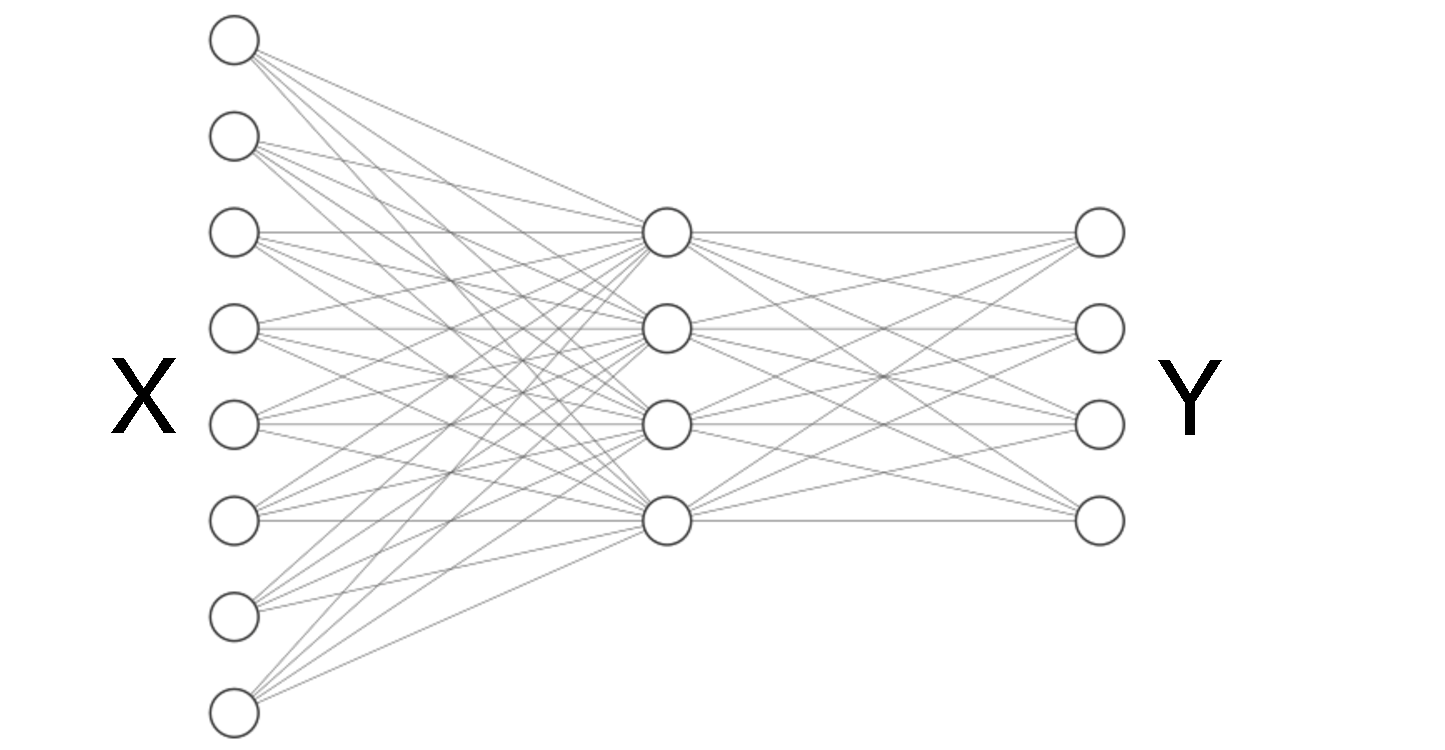
\includegraphics[width=0.7\linewidth]{images/fcnn}
	}
	\caption{Полносвязная нейронная сеть с одним скрытым слоем}
	\label{fig:fcnn}
\end{figure}

Схематически полносвязная нейронная сеть с одним скрытым слоем представлена на рис. \ref{fig:fcnn}. Нейронная сеть принимает на вход вектор входных параметров $X$ и возвращает на выходе вектор выходных параметров $Y$. Значение в нейроне на слое $i$ вычисляется как взвешенная сумма значений нейронов на слое $i - 1$ плюс смещение (bias). Таким образом значения активаций получаемые в нейронах на слое $i$ можно представить в виде 

\begin{equation}
    x_i = \sigma(W^i_{nm} \cdot x_{i - 1} + b^i_m),
\label{eq:lin_layer}
\end{equation}

где $\sigma$ - функция активации, $W^i_{nm}$ - матрица весов, $b^i_m$ - вектор смещений, $x_{i - 1}: |x_{i - 1}| = m$ - значения активаций на слое $i - 1$, а $x_{i}: |x_{i}| = n$ - значения активаций на слое $i$. Для оптимизации (обучения) параметров нейросети применяется алгоритм обратного распространения ошибки, который был одновременно разработан А.И. Галушкиным \cite{Galushkin} и П.Д.Вебросом \cite{webros_1974}. На каждой итерации алгоритма \ref{alg:backprop} происходит два прохода - прямой и обратный. Во время прямого прохода ($X \to Y$) последовательно вычисляются значения активаций $x_i$ на каждом слое. Значение активаций на последнем слое является выходным значением нейронной сети. Затем во время обратного прохода вычисляется градиент функции ошибки по параметрам каждого слоя и значения параметров обновляются методом градиентного спуска для минимизации функции ошибки. Так как нейронная сеть представляет собой сложную функцию (композицию нескольких функций) то градиент функции ошибок по параметрам $i$-ого слоя записывается следующим образом: 

\begin{equation}
    \frac{\partial L}{\partial W^i} = \frac{\partial L}{\partial x_i} \cdot  \frac{\partial x_i}{\partial W^i}
\label{eq:partial}
\end{equation}

Частная производная $\frac{\partial x_i}{\partial W^i}$ в уравнении \ref{eq:partial} вычисляется с помощью производной функции активации $\sigma$ и значения активации $x_{i-1}$ на предыдущем слое. Частная производная $\frac{\partial L}{\partial x_i}$ для выходного слоя равна производной функции ошибок по выходам нейронной сети, а для внутренних слоев также находится с использованием производной сложной функции. Таким образом алгоритм обратного распространения ошибки вычисляет градиент $\frac{\partial L}{\partial W^i}$ на основе градиента для следующего слоя $i + 1$ что позволяет за один обратный проход от выходного слоя ко входному произвести обновление параметров всех слоев нейронной сети.

\begin{algorithm}[ht]
	\SetAlgoLined
	\KwIn{$X$ - входные наблюдения, $\hat{Y}$ - ожидаемые выходные значения, $L(Y, \hat{Y})$ - функция потерь, $W$ - параметры нейронной сети}
	\KwOut{$W^{\prime}$ - новые значения параметров нейронной сети}
	\While{$L(Y, \hat{Y})$ > $\varepsilon$}{
		Выбираем $x \sim X$, $\hat{y} \sim \hat{Y}$\;
		Прямой проход: y = NN(W, x)\;
		Вычисляем ошибку предсказания: $E = L(y, \hat{y})$\;
		Обратный проход: 
		$\Delta w_{ij} = -\alpha \frac{\partial E}{\partial w_{ij}}$\;
	}
	\caption{Алгоритм обратного распространения ошибки}
	\label{alg:backprop}

\end{algorithm}

Нейронные сети получили широкое распространение в самых разных задачах таких как распознавание изображений \cite{alexnet} и анализ текстов на естественном языке \cite{bert} благодаря тому, что нейронная сеть с достаточно большим количеством параметров может выступать в качестве универсального аппроксиматора \cite{Hornik1989}. Частичным доказательством этого утверждения является теорема Колмогорова-Арнольда\cite{kolmogorov, arnold} доказывающая, что многомерная функция многих переменных может быть представлена в виде суперпозиции непрерывных функций одной переменной. 

\subsection{Обучение с подкреплением}

Принципиальная схема обучения RL алгоритмов приведена на рисунке \ref{fig:rl}. На ней RL агент взаимодействуя со средой получает от нее состояние (s $\in \mathcal{S}$), награду ($r: \mathcal{S} \times \mathcal{A} \to \mathbb{R}$), и флаг завершения эпизода (done $\in \{0, 1\}$).  В среде агент совершает действие ($a \in \mathcal{A}$) которое переводит среду в следующее состояние ($s^{\prime} \in \mathcal{S}$). В зависимости от того является ли переход из состояния $s$ в состояние $s^{\prime}$ при действии $a$ единственным или одним из возможных с распределением $p(s^{\prime},r|s,a)$, среда называется детерминированной или не детерминированной. 

\begin{figure}[ht]
	\centerfloat{
		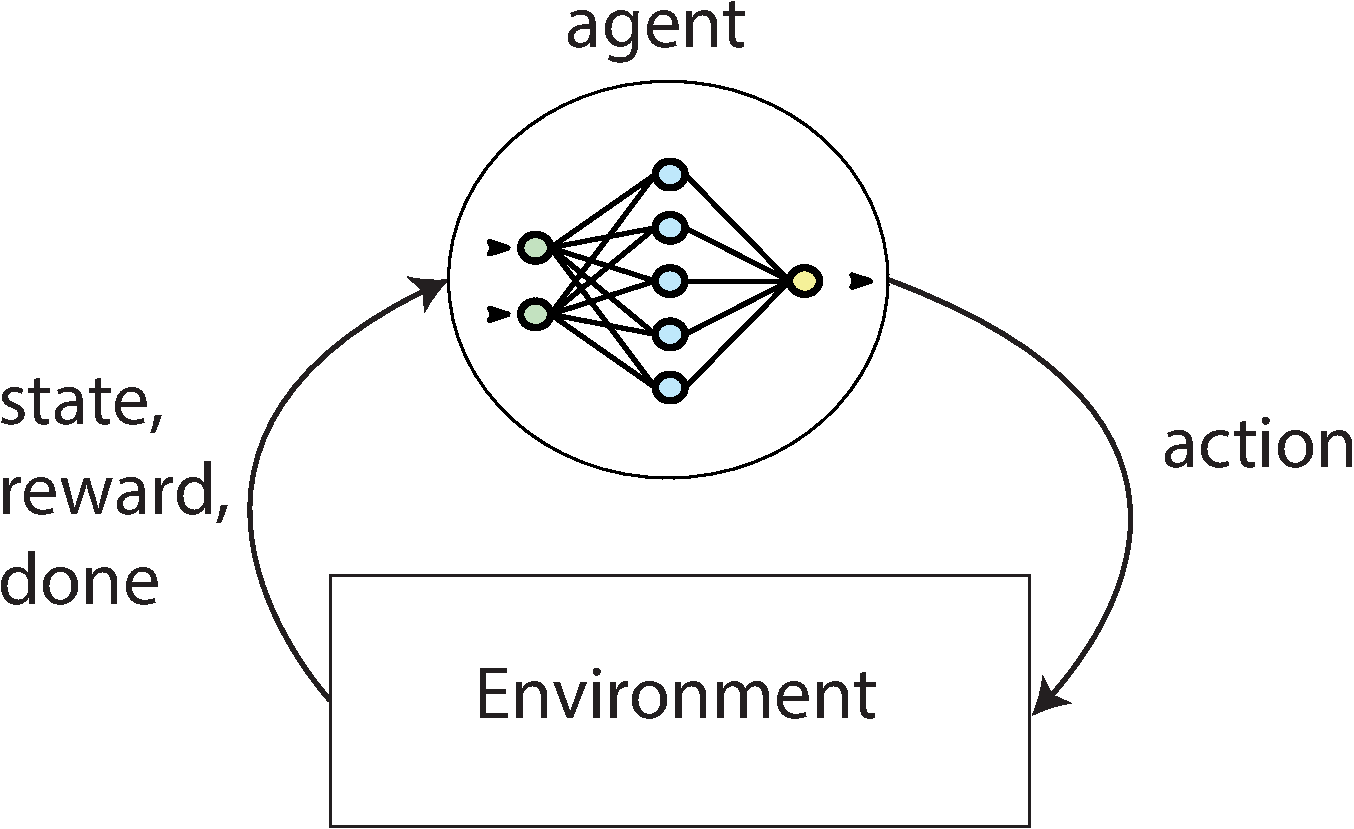
\includegraphics[width=0.5\linewidth]{images/rl_setting}
	}
	\caption{Взаимодействие агента и среды}
	\label{fig:rl}
\end{figure}

Взаимодействие RL агента со средой происходит в рамках марковского процесса принятия решений (МППР). В нем предполагается, что следующее состояние и награда получаемая агентом зависит (детерминировано или стохастически) только от предыдущего состояния и действия которое агент совершил. Если же у среды есть некоторые не наблюдаемые параметры, то говорят о частично наблюдаемом марковском процессе принятия решений (ЧНМППР). В нем наблюдение в момент времени $t$ --- $o_t \in \mathcal{O}$ определяется распределением $o_t \sim p(o_t|s_t)$, где $s_t \in \mathcal{S}$ полное состояние среды. 

Стратегия агента задается функцией $a_t=\pi(s_t)$ отображающей пространство состояний (наблюдений) в пространство действий $\mathcal{A}$. Стратегия агента может быть как детерминированной, так и стохастической. Задача агента состоит в максимизации суммарной ожидаемой дисконтированной награды к концу эпизода:

\begin{equation}
\ex_{\tau \sim \pi_{\theta}} [J(\tau)] = \ex_{\tau \sim \pi_{\theta}} [r_0 + \gamma r_{1} + \gamma ^ 2 r_{2} + ...] = \ex_{\tau \sim \pi_{\theta}} [\sum_{t} \gamma ^t r_{t}]
\end{equation}

Коэффициент $\gamma \in (0, 1]$ вводится для  ограничения эффективного горизонта --- числа шагов при котором будущая награда не влияет на стратегию из-за дисконтирования ($\gamma ^ n r$). Он также позволяет регулировать уровень жадности агента --- на сколько награда получаемая на текущем шаге ценнее аналогичной награды получаемой на следующем шаге. Математическое ожидание берется по траекториям $\tau$ полученным с помощью текущей стратегии $\pi_{\theta}$ параметризованной весами $\theta$. 
Вероятность траектории $\tau$ может быть записана следующим образом:
 
 \begin{equation}
     p(\tau|\pi) = p(s_0) \prod^T_{t=1}p(s_t|s_{t-1}, a_{t-1})\cdot \pi(a_{t-1}, s_{t-1})
\end{equation}

 где $p(s_0)$ - распределение начальных состояний в каждом эпизоде, $p(s_t|s_{t-1}, a_{t-1})$ - распределение описывающее динамику среды. Таким среда однозначно задается множеством состояний $\mathcal{S}$, действий $\mathcal{A}$, наград $\mathcal{R}$, динамикой переходов $\mathcal{R}$ и параметром $\gamma$ --- $<\mathcal{S, A, R, P}, \gamma>$.


\subsection{Уравнение Беллмана}

Ценность нахождения агента в текущем состоянии $s_t$ описывается с помощью V-функции и связанной с ней Q-функции. $V(s_t) = \ex[\sum \gamma ^t r_{t}]$ оценивает суммарную дисконтированную награду, которую получит агент находящийся в состоянии $s_t$ если он будет действовать согласно текущей стратегии. $Q(s_t, a_t) = \ex[r_t + \sum \gamma ^{t + 1} r_{t + 1}]$ оценивает суммарную дисконтированную награду, которую получит агент при совершении действия $a_t$ в состоянии $s_t$ при условии, что дальше он будет следовать текущей стратегии. С помощью V-функции можно сравнивать между собой две различные стратегии --- стратегия $\pi^{\prime}$ лучше стратегии $\pi$ если ожидаемая награда для первой стратегии $V_{\pi^{\prime}} \geq V_{\pi}$ для всех $s \in \mathcal{S}$. Таким образом можно определить оптимальную стратегию $\pi^*: V_{\pi^*} \geq  V_{\pi} \  \forall \pi$. Значения V, Q-функций в точках $s_t$ и $s_{t + 1}$ при условии, что текущая стратегия является оптимальной связаны между собой уравнениями Беллмана: 

\begin{equation}
	V^*(s) = \max_{a \in \mathcal{A}} \ex(r_{t + 1} + \gamma V^*(s_{t + 1}))
\end{equation}

\begin{equation}
Q^*(s, a) = \ex(r_{t + 1} + \gamma \max_{a' \in \mathcal{A}} Q^*(s_{t + 1}, a'))
\end{equation}

Значения оптимальных V, Q-функций связаны между собой: 

\begin{equation}
V^*(s) = \max_{a \in \mathcal{A}}Q^*(s, a)
\end{equation}

Смысл V-функции можно легко интерпретировать в задаче изображенной на рис. \ref{fig:minigrid}. В ней агент движется из верхнего левого угла ($s_0$) сетки в правый нижний угол ($s_f$). Если агент за каждый шаг получает награду $r = -1$, то оптимальная V-функция при условии того, что коэффициент дисконтирования $\gamma = 1$ в состоянии $s_t$ будет равна числу действий необходимых для достижения состояния $s_f$ взятых со знаком ``-''. 

\begin{figure}[ht]
	\centerfloat{
		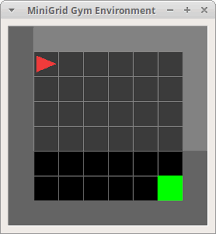
\includegraphics[width=0.3\linewidth]{images/minigrid_empty}
	}
	\caption{Среда MiniGrid-Empty-8x8-v0 \cite{gym_minigrid}}
	\label{fig:minigrid}
\end{figure}

 
\subsection{Метод value iteration}

Уравнения Беллмана могут быть использованы для построения оптимальной стратегии для сред с конечным набором состояний и известным распределением переходов между ними $p(s^{\prime}, r|s, a)$. Метод value iteration \ref{alg:value_it} строится на применении метода простой итерации к уравнению Беллмана для V-функции. Данный метод имеет гарантированную сходимость \cite{Sutton1998}, но может быть использован только для очень ограниченного набора задач.

\begin{algorithm}[ht]
	\SetAlgoLined
	\KwIn{$t$ - условие останова, $\mathcal{S}$ - набор состояний среды, $p(s^{\prime}, r|s, a)$ - распределение вероятности переходов}
	\KwOut{$\pi(s) = \mathrm{argmax}_{a} \sum_{s', r}p(s',r|s,a)[r + \gamma V(s')]$}
	Инициализируем V(s) = 0 (для всех $s \in \mathcal{S}$), $\Delta = \infty$\;
	\While{$\Delta$ > t}{
		$\Delta$ = 0\;
		\ForEach{s $\in \mathcal{S}$}{
		    $V_{old}$ = V(s)\\
		    %V_{old}(s) = V(s)\par
			V(s) = $\max_a \sum_{s', r}p(s', r|s, a)[r + \gamma V(s')]$\\
			$\Delta = \max(\Delta, |V_{old} - V(s)|)$
		}
	}
	\caption{Алгоритм value iteration}
	\label{alg:value_it}

\end{algorithm}

В рамках данной работы были использованы алгоритмы глубокого обучения с подкреплением, обучающиеся методом проб и ошибок и не строящие в явном виде моделей награды и переходов среды. В зависимости от того, как используются данные полученные от среды такие алгоритмы можно разделить на два больших класса on-policy и off-policy. В on-policy алгоритмах агент обучается на данных, полученных с помощью текущей стратегии. Благодаря этому получается добиться большей стабильности обучения, но требуется гораздо больше данных так как нет возможности переиспльзовать данные полученные при взаимодействии устаревшей стратегии со средой. 
В off-policy алгоритмах агент выучивает оптимальную стратегию (Q-функцию) используя исторические данные взаимодействия со средой полученные при использовании предыдущих версий стратегии. 

\subsection{Off-policy алгоритмы}

\paragraph{Алгоритм DQN}

Одними из наиболее популярных методов основанных на приближенном вычислении Q-функции являются алгоритмы Q-learning \cite{Watkins_1992} и Deep Q-learning \cite{mnih2013atari}. В методе Q-learning функция $Q(s, a)$ иттеративно обновляется на основании опыта собранной текущей стратегией. В работе \cite{SuttonQLearning} показано, что функция обновляемая таким методом сходится к оптимальной Q-функции.

Существенный прорыв в методах основанных на Q-обучении был достигнут в 2015 году. Благодаря использованию нейронных сетей в качестве аппроксиматора для Q-функции авторами \cite{mnih2013atari} был разработан метод DQN который обучился играть в 49 игр Atari на уровне человека. Игры Atari рассматриваются в качестве одного из основных тестов для сравнения качества работы различных алгоритмов основанных на глубоком обучении с подкреплением.  

Алгоритм DQN строится на обучении глубокой нейронной сети аппроксимировать Q-функцию для каждого возможного действия в зависимости от текущего состояния игры --- изображения или последовательности изображений 84x84 пикселя. Для стабилизации процесса обучения Q-функции авторы использовали следующее выражение для функции потерь:

\begin{equation}
    L(\theta) = \ex_{<s, a, r, s^{\prime}> \sim \mathcal{D}}\left[\left(r + \gamma \max_{a^{\prime}}
    Q_{\theta^-}(s^{\prime}, a^{\prime}) - Q_{\theta}(s, a)\right)^2 \right]
\label{eq:dqn}
\end{equation}

Буфер $\mathcal{D}$ содержит состояния и действия полученные при взаимодействии со средой $<s, a, r, s^{\prime}>$. В уравнении \ref{eq:dqn} для вычисления Q-значения в следующем состоянии $s^{\prime}$ используется скользящее средние весов Q-функции что позволяет стабилизировать обучение и делает алгоритм DQN эффективным для решения многих задач обучения с подкреплением.

Для заданной Q-функции стратегия агента определяется $\varepsilon$-жадным способом: 

\begin{equation}
    \pi =  \begin{cases}
      \mathrm{argmax}_{a}(Q(s, a)) & \text{если $\zeta \sim$ U(0, 1) > $\varepsilon$}\\
      a \sim \mathcal{A} & \text{иначе}
    \end{cases}       
\end{equation}

При каждом шаге взаимодействия со средой во время обучения выбирается случайное число $\zeta \sim U(0, 1)$ и если оно больше параметра $\varepsilon$, то агент использует свое знание о среде -- выбирает действие с большим значением Q-функции. Если же $\zeta < \varepsilon$, то агент исследует среду выбирая случайное действие.  

\paragraph{Алгоритм TD3}
Существенным ограничением метода DQN является то, что он применим исключительно для сред с дискретным набором действий так как для выбора действия в стратегии используется максимум по действиям значений Q-функции. Также одной из проблем, возникающих при аппроксимации Q-функции с использованием нейронных сетей является частая переоценка значений Q-функции в большую сторону.

Одним из наиболее популярных алгоритмов применяемых в условиях марковского процесса принятия решений с использованием непрерывного пространства действий является алгоритм TD3 \cite{Fujimoto2018AddressingFA}. Алгоритм TD3 использует три нейронных сети: первая (актор) для задания детерминированной стратегии агента $\pi_{\theta}$ и две оставшиеся (критики) для оценки значений $Q_{\theta_1}, Q_{\theta_2}$. 
Обе Q-функции обучаются при минимизации ошибки с одной целевой функцией, вычисляемой с использованием наименьшего из значений Q-функций:

\begin{equation}
    y(r, s^{\prime}) = r + \gamma \min(Q_{\theta_1}(s^{\prime}, \pi_{\theta}(s^{\prime})), Q_{\theta_2}(s^{\prime}, \pi_{\theta}(s^{\prime})))
\label{eq:double_q}
\end{equation}

\begin{equation}
    L(\theta_1, \mathcal{D}) = \ex_{<s, a, r, s^{\prime}> \sim \mathcal{D}}\left[\left(Q_{\theta_1}(s, a) - y(r, s)\right)^2 \right]
\end{equation}

\begin{equation}
    L(\theta_2, \mathcal{D}) = \ex_{<s, a, r, s^{\prime}> \sim \mathcal{D}}\left[\left(Q_{\theta_2}(s, a) - y(r, s)\right)^2 \right]
\end{equation}

В формуле \ref{eq:double_q} используется минимум из двух Q-функций позволяет уменьшить переоценку Q-значений. Дополнительно во время обучения алгоритм TD3 сглаживает значения Q-функции при помощи случайного шума, который добавляется в действия $a \to a + \mathcal{N}(0, 1)$ при обновлении параметров нейронных сетей критиков. 

Стратегия агента обучается максимизировать значение $Q_{\theta_1}$ в состоянии $s$:

\begin{equation}
    \max_{\phi}\ex_{s \sim \mathcal{D}}\left(Q_{\theta_1}(s, \pi_{\phi}(s))\right)
\end{equation}

Для стабилизации процесса обучения нейронная сеть определяющая текущую стратегию агента обновляется реже чем нейронные сети вычисляющие Q-функции. Также в каждой действие в процессе обучения агента добавляется случайный шум для лучшего исследования среды. 

Алгоритм TD3 представляет собой обобщение алгоритма DQN на случай непрерывного пространства действий. Благодаря тому, что TD3, как и DQN способен обучаться на исторических данных он требует меньшего количества данных для обучения чем on-policy алгоритмы.

\subsection{On-policy алгоритмы}

Одной из проблем off-policy методов является то, что хорошая оценка Q-функции не является гарантией оптимальности стратегии агента. 
Это можно представить на примере среды, содержащей только два действия $a_1, a_2$. Рассмотрим две стратегии $Q_1, Q_2$ и оптимальную стратегию $Q^*$ в начальном состоянии $s_0$: 

\begin{equation}
    Q_1(s_0, a) = 
    \begin{cases}
    6 & \text{if $a = a_1$}\\
    5 & \text{otherwise}
    \end{cases}
\end{equation}

\begin{equation}
    Q_2(s_0, a) = 
    \begin{cases}
    7 & \text{if $a = a_1$}\\
    10 & \text{otherwise}
    \end{cases}
\end{equation}

\begin{equation}
    Q^*(s_0, a) = 
    \begin{cases}
    5 & \text{if $a = a_1$}\\
    6 & \text{otherwise}
    \end{cases}
\end{equation}

Стратегия задаваемая $Q_2$ будет выбирать оптимальное действие $a_2$ несмотря на то, что ошибка измеряемая квадратичной функцией потерь у нее существенно больше чем у $Q_1$ которая будет выбирать не оптимальное действие $a_1$: 

\begin{equation*}
    L_1 = \sum_a(Q_1 - Q^*)^2 = 2
\end{equation*}

\begin{equation*}
    L_2 = \sum_a(Q_2 - Q^*)^2 = 20
\end{equation*}

Решением этой проблемы может быть оптимизация параметров стратегии напрямую. Так как целью агента является максимизация ожидаемой суммарной дисконтированной награды:

\begin{equation}
    J(\pi) = \ex_{\tau\sim \pi}\left[ R(\tau) \right] = \ex_{\tau\sim \pi}\left[ \sum_t \gamma^t r_t \right]
\label{eq:exp_ret}
\end{equation}

В on-policy методах стратегия агента $\pi$ для определяет распределение вероятностей действий для каждого состояния. Для оптимизации нужно определить градиент ожидаемой награды по параметрам стратегии. Эта связь задается следующей теоремой:

\paragraph{Теорема градиента стратегии} Градиент ожидаемой награды по стратегии равен математическому ожиданию произведения награды на градиент логарифма стратегии $\pi_{\theta}$:

 
\begin{multline}
    \nabla_{\theta} J(\pi_{\theta}) = 
    \nabla_{\theta} \sum_{\tau \sim \pi}\left[\pi_{\theta}(\tau) R(\tau)\right] = 
    \sum_{\tau \sim \pi}\left[\pi_{\theta}(\tau) \frac{\nabla_{\theta} \pi_{\theta}(\tau)}{\pi_{\theta}(\tau)} R(\tau)\right] = \\
    \ex_{\tau \sim \pi}\left[\nabla_{\theta}\log{\pi_{\theta}(\tau)} R(\tau)\right]
\label{eq:polgrad}
\end{multline}

Величина суммарной награды $R(\tau)$ часто имеет большой разброс и соответственно градиент \ref{eq:polgrad} будет шумным. Для того чтобы стабилизировать процесс обучения вместо суммарной награды в уравнении \ref{eq:polgrad} используется величина называемая Generalized Advantage Estimate (GAE) \cite{Schulman2016HighDimensionalCC}. 

\paragraph{Generalized Advantage Estimate}
Запишем оценку состояния с использованием информации о награде за $n$-шагов:

\begin{equation}
    V^{\prime}(s_t) = r_t + \ldots + \gamma^{n-1} r_{t+n-1} + \gamma^{n}V(s_{t+n})
\end{equation}

Выбор параметра $n$ важен, так как оценка $V^{\prime}(s_t)$ имеет большое смещение при маленьком значении параметра $n$ и большой разброс при большом значении параметра $n$. Величиной Advantage называется разница между первоначальной оценкой состояния $V(s_t)$ и оценкой $V^{\prime}(s_t)$:

\begin{equation}
    \mathrm{Adv}_n = \sum_{t^{\prime} = t}^{t+n-1} \gamma^{t^{\prime} - t}r_{t^{\prime}} + \gamma^{n}V(s_{t+n}) - V(s_t) = \sum_{l = 0}^{n-1}\gamma^l\delta_{t+l},
\end{equation}
где $\delta_t^V = r + \gamma V(s_{t+1}) - V(s_t)$ --- временная разность определяющая на сколько получаемая награда отличается от нашей первоначальной оценки. Величина GAE задается следующим уравнением: 

\begin{equation}
    A_t = \sum_{l = 0}^{\infty}(\gamma \lambda)^l \delta_{t+l}^V
\end{equation}

GAE с помощью параметра $\lambda \in [0, 1]$ позволяет контролировать смещение и разброс. $A_t = \delta_t$ при $\lambda = 0$ что соответствует оценке с одним шагом ($n = 1$). $A_t = \sum_{l=0}^{\infty} \gamma^lr_{t+l} - V(s_t)$ при $\lambda = 1$ что соответствует оценке методом Монте-Карло c $n \to \infty$. 

\paragraph{Алгоритм PPO}

PPO --- один из лучших on-policy алгоритмов. Он подходит как для сред с дискретными, так и с непрерывными действиями. В процессе обновления стратегии лежит следующая идея: сделать максимально возможный шаг по улучшению стратегии, не заходя слишком далеко, чтобы не вызвать снижения качества работы. PPO использует две нейронные сети --- актор $\pi_{\theta}(\cdot|s)$ и критик $V_{\phi}(s)$ \cite{Schulman2017ProximalPO}. Нейронная сеть критика обучается предсказывать ценность текущего состояния $s$ с помощью квадратичной функции ошибок: 

\begin{equation}
    L(\phi) = \ex_{\tau \sim \pi}\left[\left(r + \gamma V_{\phi}(s^{\prime}) - V_{\phi}(s)\right)^2 \right]
\end{equation}

Нейронная сеть актора $\pi_{\theta} (\cdot|s_i)$ минимизирует следующий функционал: 

$$
L(\theta) = \ex_{\tau \sim \pi_{k}} \left[ \sum_{t = 0}^{T} \min(\rho_{t}(\theta)A_t,\mathrm{clip}(\rho_t(\theta), 1 - \varepsilon, 1 + \varepsilon)A_t) \right]
$$


где $\rho_t(\theta) = \pi_{\theta}(a_t|s_t) / \pi_{\theta^{\prime}}(a_t|s_t)$ – отношение вероятностей действия $a_t$ в состоянии $s_t$ для текущей $\pi_{\theta}$ стратегии и стратегии $\pi_{\theta^{\prime}}$ использовавшейся при совершении действия $a_t$ в среде; функция clip ограничивает $\rho_t(\theta)$ значением $1 - \varepsilon$ снизу и значением $1 + \varepsilon$ сверху; $A_t$ - Generalized Advantage Estimate.

Наиболее важной частью алгоритма PPO является функция ошибок для актора. Рассмотрим ее работу в двух случаях $A_t \geq 0$ и $A < 0$. В случае $A_t \geq 0$:

\begin{equation}
    L(\theta, a, s) = \min(\rho(\theta, a, s), 1 + \varepsilon)A(a, s)
\end{equation}

Так как advantage является положительным, то функция потерь вырастет если вероятность действия увеличится $\pi_{\theta}(a|s)$. Но оператор $\min$ ограничивает величину функции потерь значением $1 + \varepsilon$. Что приводит к тому, что новая стратегия $\pi_{\theta}$ не сильно отклоняется от предыдущей $\pi_{\theta^{\prime}}$. 

Аналогичный эффект произойдет для случая отрицательного advantage --- оператор $\max$ ограничивает
величину функции потерь величиной $1 - \varepsilon$:

\begin{equation}
    L(\theta, a, s) = \max(\rho(\theta, a, s), 1 - \varepsilon)A(a, s)
\end{equation}

\subsection{Использование внутренней мотивации в средах с редкой наградой}

Итоговое качество работы RL агента во многом зависит от того, насколько хороший сигнал он получает при взаимодействии со средой. Если агент получает награду слишком редко (т.е. сигнал поступающий от среды является разреженным), то исследование среды посредством совершения случайных действий будет не эффективным. Для обучения RL агента в подобных условиях добавляют дополнительную награду, которая побуждает агента к исследованию среды. Данная награда получила название внутренней мотивации. 

Большинство наиболее популярных методов внутренней мотивации можно разделить на два класса: методы основанные на подсчете количества посещений состояний (count-based methods) мотивирующие агента посещать новые состояния и методы основанные на любопытстве (curiosity-based methods) мотивирующие агента исследовать динамику среды. 

\paragraph{Count-based методы} Наиболее просто задать награду за посещение новых состояний в табличных средах --- средах с дискретным набором состояний. В работе \cite{Strehl2008} было предложено использовать счетчики посещения состояний в качестве дополнительной награды в табличных средах. 

В средах в которых состояния являются изображениями задача существенно усложняется. Одним из наиболее эффективных алгоритмов внутренней мотивации применяемых в задачах с состояниями высокой размерности является метод random network distilation \cite{rnd}.
В работе \cite{rnd} для определения награды использовались две нейронные сети. Первая сеть была инициализирована случайным образом и не обучалась представляя собой случайное преобразование из пространства состояний в пространство меньшей размерности. Вторая же сеть обучалась минимизировать среднеквадратичную ошибку между своим предсказанием и предсказанием первой сети. В качестве награды выступает квадрат ошибки вычисляемый между предсказаниями двух нейронных сетей. Мотивация данного метода состоит в том, что случайное преобразование задаваемое первой нейронной сетью будет отображать близкие состояния среды в близкие представления, а различные --- в далекие. Таким образом ошибка предсказания получаемая второй обучающейся нейронной сетью будет изначально большой для новых состояний и будет убывать по мере обучения для часто посещаемых состояний. 
Для процедурно генерируемых сред таких как игра Nethack \cite{nethack} методы внутренней мотивации основанные на подсчете посещений состояний могут быть не эффективны, так как каждый раз среда генерируется заново и вероятность оказаться в похожем состоянии мала.

\paragraph{Curiosity-based методы} Методы основанные на любопытстве мотивируют агента исследовать среду через изучение ее динамики. Любопытство может быть определено как ошибка или неопределенность в предсказании поведения среды при условии действия и текущего состояния $p(s, a)$ \cite{stadie2015incentivizing, pathak2017curiosity} В работе \cite{pathak2017curiosity} использовалась нейронная сеть, которая училась предсказывать латентное представление следующего состояния, а в качестве награды агенту давалась ошибка между предсказанием и латентным представлением следующего состояния полученным от среды. В этом подходе агент получает награду не за посещение новых состояний, а за то, что его действия в среде приводят к неожиданным состояниям. Данный метод не очень хорошо работает для сред со стохастической динамикой. В таких средах агент будет получать случайные награды, которые могут затруднить исследование среды. 


\subsection{Мета-обучение}\label{sec:ch1/sec1/subsec8}

RL агент взаимодействует со средой как во время обучения, так и во время тестирования. Обычно, методы обучения с подкреплением предназначены для решения конкретной задачи и не могут легко обобщаться на другие похожие задачи. Для того чтобы обучить агента решению другой задачи, его обучение приходится начинать заново. Таким образом для обучения многих агентов требуется большое количество данных, что не является эффективным.

Мета-обучение позволяет агенту научиться адаптироваться к различным задачам. В базовой постановке задачи мета-обучения рассматривается распределение задач $p(\mathcal{T})$, из которого в течении процесса мета-обучения случайным образом выбирается задача $\mathcal{T}$. Разные задачи могут отличаться функцией награды и динамикой среды $p(s^{\prime}|s, a)$, но их должна объединять некоторая структура.
В общем случае алгоритм мета-обучения состоит из двух циклов оптимизации --- внешнего и внутреннего. 
Во внутреннем цикле оптимизации алгоритм адаптируется к выбранной задаче $\mathcal{T}$, в то время как во внешнем цикле он обобщается на все распределение задач $p(\mathcal{T})$. Во время тестирования мета-агента тестовая задача выбирается случайным образом из всего распределения $p(\mathcal{T})$ и агент в течении нескольких эпизодов взаимодействия со средой должен адаптироваться к выбранной задаче. После этого измеряется средняя суммарная награда. Для тестирования на следующих задачах параметры агента возвращаются к своим первоначальным значениям. Алгоритмы мета-обучения различаются процедурой используемой для адаптации к задаче \cite{meld}: вероятностный вывод  \cite{PEARL, VariBad},  рекуррентное обновление \cite{meld, RL2} или градиентное обновление \cite{maml}. 

Сравнение различных алгоритмов мета-обучения приведено в работе \cite{yu2020meta}. В сравнении показано, что существующие на данный момент алгоритмы мета-обучения не могут в полной мере эффективно обобщаться на существенно отличающиеся задачи и испытывают сложности при обучении одновременно нескольким существенно отличающимся задачам.

%Далее рассмотрим PEARL  \cite{PEARL} как один из наиболее эффективных алгоритмов вероятностного вывода и MAML \cite{maml} как один из лучших алгоритмов основанных на градиентном обновлении. 

%Алгоритм PEARL разделяет две задачи --- идентификацию задач и оптимизацию стратегии агента. Этот подход совместно с использованием off-policy алгоритма во внутреннем цикле оптимизации увеличивает эффективность алгоритма по сравнению с рекуррентными и методами основанными на градиентном обновлении алгоритмами мета-обучения. Для определения задачи алгоритм PEARL использует вариационный амортизированный подход \cite{vae, vae2014, vae2016} для того, чтобы научиться определять латентный вектор контекста  $z$, который кодирует смысловую информацию о задаче. Для непосредственного решения задачи во внутреннем цикле оптимизации используется алгоритм Soft Actor-Critic (SAC) \cite{sac, sac_applications}. На вход ему подается наблюдение $s$ объединенное с вектором контекста $z$. 
%Нейронная сеть предназначенная для определения задачи возвращает распределение $q_{\phi}(z|c^{\mathcal{T}})$, которое аппроксимирует апостериорное распределение $p(z|c^{\mathcal{T}})$, вектор контекста $c^{\mathcal{T}}$ включает в себя опыт собранный к текущему моменту для задачи $\mathcal{T}$. Вектор контекста определяется как набор $\{c^{\mathcal{T}}_{1:N}\}$, где $c^{\mathcal{T}}_{n} = \{s_{n}, a_{n}, r_{n}, s'_{n}\}$ один переход в рамках задачи данной задачи. Распределение $q_{\phi}(z|c^{\mathcal{T}})$ является инвариантным к перестановкам:

%\begin{equation}\label{eq:qzc}
%    q_{\phi}(z|c^{\mathcal{T}}) = \prod_{n=1}^{N} %\mathcal{N}(f^{\mu}_{\phi}(c_{n}^{\mathcal{T}}), %f^{\sigma}_{\phi}(c_{n}^{\mathcal{T}})),
%\end{equation}

%Благодаря этому латентный вектор $z$ обучается сохранять информацию о задаче, а не о конкретной траектории. В уравнении выше функции $f^{\mu}_{\phi}(\cdot)$ и $f^{\sigma}_{\phi}(\cdot)$ предсказывают среднее значение и дисперсию гауссовского распределения $\mathcal{N}(\cdot,\cdot)$ как функции от $c_{n}^{\mathcal{T}}$. Параметры нейронной сети $q_{\phi}(z|c^{\mathcal{T}})$ совместно с параметрами нейронной сети актора $\pi_{\theta}(a|s, z)$ и критика $Q_{\theta}(s, a, z)$ оптимизируются с использованием метода  репараметризации \cite{vae}. Функция потерь для нейронной сети предсказывающей задачу состоит из двух слагаемых: KL-дивергенция между $q_{\phi}(z|c^{\mathcal{T}})$ и стандартным нормальным распределением  и ошибка соответствующая уравнению Беллмана для нейронной сети критика. Обучение нейронной сети критика приводит к тому, что вектор $z$ обучается кодировать необходимую информацию о решаемой задаче. 

%В течении мета-теста, задача $\mathcal{T}$ случайным образом выбранная из распределения задач фиксируется для заданного числа эпизодов взаимодействия со средой, и создается пустой массив для хранения векторов контекста $c^\mathcal{T} = \{\}$. В начале каждого эпизода, агент делает гипотезу о задаче при выборе вектора  $z \sim q_{\phi}(z|c^\mathcal{T})$. Далее, агент собирает данные $D^\mathcal{T} = \{(s_{n}, a_{n}, r_{n}, s'_{n})\}_{1:{\mathrm{episode\_length}}}$ с помощью стратегии  $\pi(a| s, z)$ , которые затем добавляются в контекст $c^\mathcal{T} \leftarrow c^\mathcal{T} \cup D^\mathcal{T}$. Латентный вектор $z$ является постоянным в течении всего эпизода, что позволяет агенту тестировать гипотезы независимо от задачи. В процессе тестирования размер $N$ вектора контекста растет и произведение гауссиан уменьшается (\ref{eq:qzc}), что позволяет точно оценить значение латентного вектора $z$.

%Алгоритм MAML ищет оптимальную инициализацию нейронной сети актора для всех задач из распределения для того, чтобы достичь быстрой адаптации (few-shot learning) в процессе мета-теста. В процессе мета-обучения, во внутреннем цикле алгоритм MAML совершает один шаг алгоритма оптимизации стратегии для каждой задачи $\mathcal{T}$ с использованием метода policy gradient и generalised advantage estimation \cite{gae}. Во внешнем цикле оптимизации алгоритм MAML оптимизирует параметры стратегии для того, чтобы за один шаг внутреннего цикла оптимизации получить наибольший прирост качества работы стратегии, усредненный по всем задачам. В течении мета-теста, агент использует внутренний цикл для оптимизации весов к конкретной решаемой задаче. 

\subsection{Иерархические методы обучения с подкреплением}

Многие задачи возникающие в реальности имеют иерархическую структуру. Например, в задаче управления шагающим роботом стратегия нижнего уровня может уметь приходить в заданную координату, а стратегия верхнего уровня использует ее для того, чтобы обойти препятствия или перемещать грузы \cite{robel}. В игре Nethack общая стратегия может быть построена на основе стратегий предназначенных для решения конкретных задач и переключаться между ними в зависимости от текущего состояния \cite{confbib3}. Разработка RL агентов, которые могут выучивать иерархические стратегии (HRL) является важной задачей в обучении с подкреплением \cite{Sutton1999, dietterich2000hierarchical, mcGovern}. Большинство HRL алгоритмов подходят или только для дискретных сред, требуют предобученные стратегии нижнего уровня или строят модели среды. Иерархический RL также может показывать лучшие результаты в задачах навигации с разреженной наградой. В таких задачах стратегия нижнего уровня должна прийти в состояние заданное стратегией верхнего уровня которая обучается генерировать достижимые целевые состояния. 

В работе \cite{levy2017learning} реализован алгоритм иерархического обучения с подкреплением в котором различные уровни иерархии обучаются одновременно. В качестве задач (состояний которые должны быть достигнуты промежуточными стратегиями, $g$) используются дискретные состояния среды. Для того чтобы учить различные уровни иерархии одновременно, цели уже после совершения действий подменяются следующим образом: 

\begin{equation}
    \pi_i(s|g) \sim [(s_1,a_1,r_1,g), \ldots (s_n,a_n,r_n,g)] \to \begin{cases}
        g & \text{если $s_n = g$}\\
        s_n & \text{если $s_n \neq g$}\\
    \end{cases}
\end{equation}
Этот подход позволяет обучать промежуточные стратегии $\pi_i$, даже если стратегии еще $\pi_{i+1}$ не научились генерировать достижимые цели. К минусам этого подхода можно отнести то, что он не подходит для состояний высокой размерности таких как изображения, так как их нельзя напрямую сравнивать напрямую между собой. 

%//TODO FIXME
%Метод иерархического обучения с подкреплением способный работать с изображениями и одновременно обучать стратегии верхнего и нижнего уровня представлен в работе \cite{hafner2022deep}. В ней используется модель среды обученная по состоянию и действию предсказывать следующее состояние среды: 

%\begin{equation*}
%    \mathrm{WorldModel}(s_t, a) = s_{t+1}
%\end{equation*}

%С использованием модели среды обучаются две стратегии --- верхнего и нижнего уровня. Стратегия верхнего уровня выбирает задачу на фиксированное число шагов, а стратегия нижнего уровня обучается ее достигать. В качестве задач используются дискретные представления полученные с помощью автокодировщика --- отдельной нейронной сети обученной сжимать и восстанавливать исходное изображение из меньшего объема данных \cite{vqvae}. Стратегия верхнего уровня выбирает дискретные представления, которые затем с помощью автокодировщика преобразуются в изображения и подаются на вход стратегии нижнего уровня в качестве текущей задачи. 

\section{Обзор применения методов обучения с подкреплением в роботике}\label{sec:ch1/sec2}

В настоящее время роботы успешно справляются с четко поставленными задачами в условиях неизменного внешнего окружения. Примерами таких задач являются автоматизация конвейерных линий сборки автомобилей или различных устройств. Также в бытовых условиях, где окружение меняется ежедневно, но незначительно, современные роботы – например, пылесосы или голосовые помощники – находят свое применение. Однако, в сильно недетерминированных средах или в областях, где требуется многозадачность, роботы все еще сильно уступают человеку. Причин этому множество, начиная со слабой степени развития некоторых типов сенсоров, например, тактильных, которые должны передавать роботу информацию об окружающей среде, и заканчивая отсутствием интеллектуальных самообучающихся алгоритмов, которые были бы способны быстро адаптироваться к изменяющемуся окружению после лишь нескольких взаимодействий с ним. 

Искусственный интеллект призван заменить жесткие программы, разработанные человеком, для управления роботами. Конечной целью исследований в области искусственного интеллекта является создание безопасного для человека общего искусственного интеллекта (Artificial general intelligence - AGI). Важную роль в создании AGI играют методы обучения с подкреплением и глубокие нейронные сети. 
Наиболее общим методом создания алгоритмов искусственного интеллекта для роботов является обучение с подкреплением. В рамках RL для управления роботом требуется найти оптимальную алгоритм принятия решения о действии –-- стратегию, зависящую от текущего состояния робота, которая бы приводила к достижению цели. Использование методов RL позволяет роботу самостоятельно выучить оптимальную последовательность действий и получить такую стратегию, которая бы могла работать с шумами во входных данных. Среди остро стоящих на данный момент задач управления роботами с помощью алгоритмов RL можно выделить следующие:

\paragraph{Sim2Real} --- перенос стратегии, обученной на симуляции в реальную среду. Так как изначально нейронная сеть не имеет никакого представления о среде, то большинству методов обучения с подкреплением требуются миллионы взаимодействий со средой, чтобы выучить оптимальную стратегию. Скорость обучения на реальном роботе ограничена временем отклика механических манипуляторов, что составляет от долей до нескольких секунд. Поэтому обучение часто проводится в компьютерной симуляции, а затем переносится на реального робота. При этом могут возникнуть проблемы, связанные с тем, что даже самая детальная симуляция не способна воспроизвести динамику реальной среды полностью. 

\paragraph{Few shot / Meta learning} --- обучение на непродолжительном взаимодействии со средой. Человеку требуется значительно меньше опыта для выполнения новой задачи, чем любому из известных алгоритмов обучения с подкреплением. Это связано с тем, что человек имеет большой априорный опыт о динамике среды. Суть мета-обучения заключается в предобучении агента решать задачи из некоторого распределения (например, ходить по поверхностям с разным коэффициентом трения, ходить вперед/назад, поворачиваться по/против часовой стрелки; см. раздел \ref{sec:ch1/sec1/subsec8}). Предобученный агент затем способен дообучиться под конкретную задачу с использованием небольшого опыта взаимодействия со средой. 

\paragraph{Policy adaptation} --- Адаптация стратегии к внезапным изменениям в динамике среды (гололед на поверхности) или изменениям в конструкции робота (внезапный отказ одного или нескольких сервоприводов). При выполнении задач в реальных условиях возможны отказы различных элементов робота или изменение внешних условий. Работоспособности робота может помочь разработка специальных методов обучения, способных адаптироваться к изменениям конфигурации робота и изменению окружения в режиме реального времени без продолжительного дообучения или обслуживания робота. Подобные методы крайне востребованы, т. к. приближают действия робота к поведению человека в реальных жизненных ситуациях.

\paragraph{Curse of demensionality}

Термин проклятие размерности был предложен Ричардом Беллманом в 1957 году, когда он столкнулся с экспоненциальным ростом количества состояний и действий в задачах оптимального управления в пространствах высокой размерности. Робототехнические системы часто имеют дело с состояниями и действиями высокой размерности. Так например в задаче управления четвероногим роботом размерность пространства состояний обычно составляет от 100 до 200, а размерность действий совпадает с числом суставов робота. 

\paragraph{Curse of goal specification}
В обучении с подкреплением желаемое поведения неявно задается с помощью функции награды. Целью RL агента является максимизация суммарной награды. Несмотря на то, что задать награду значительно проще чем желаемое поведение на практике задать хорошую функцию награды может быть проблематично так в работе \cite{hwangbo2019learning} функция награды содержит 8 - 10 слагаемых (в зависимости от задачи) регулирующих желаемое поведение агента. 
Во многих задачах естественным образом заданная награда является бинарной сигнализирующей о достижении или не достижении заданной цели. Например, для шагающего робота такой наградой может быть индикатор того, пришел ли он в заданную координату. Однако такая награда не является оптимальной для обучения агента так как в процессе обучения RL агент может ни разу ни встретить эту награду. 
С другой стороны при задании плотной награды агент может найти такое поведение, которое бы эксплуатировало не оптимально заданную награду. Это чаще всего происходит когда в награде есть положительные циклы --- пути в пространстве состояний и действий в которых агент возвращается в начальное состояние и получает при этом положительную награду. 


%\section{Ссылки}\label{sec:ch1/sec2}


\FloatBarrier
           % Глава 1
\chapter{Настройка оптического интерферометра методами машинного обучения с подкреплением}\label{ch:ch2}

\section{Физические принципы работы оптического интерферометра}\label{sec:ch2/sec1}

\begin{figure}[ht]
    \centerfloat{
        \includegraphics[scale=0.27]{latex}
    }
    \caption{TeX.}\label{fig:latex}
\end{figure}

Для выравнивания изображения по-центру используется команда \verb+\centerfloat+, которая является во
многом улучшенной версией встроенной команды \verb+\centering+.

\section{Настройка оптического интерферометра как задача машинного обучения с подкреплением}\label{sec:ch2/sect2}

А это две картинки под общим номером и названием:
\begin{figure}[ht]
    \begin{minipage}[b][][b]{0.49\linewidth}\centering
        \includegraphics[width=0.5\linewidth]{knuth1} \\ а)
    \end{minipage}
    \hfill
    \begin{minipage}[b][][b]{0.49\linewidth}\centering
        \includegraphics[width=0.5\linewidth]{knuth2} \\ б)
    \end{minipage}
    \caption{Очень длинная подпись к изображению,
        на котором представлены две фотографии Дональда Кнута}
    \label{fig:knuth}
\end{figure}

Те~же~две картинки под~общим номером и~названием,
но с автоматизированной нумерацией подрисунков:
\begin{figure}[ht]
    \centerfloat{
        \hfill
        \subcaptionbox[List-of-Figures entry]{Первый подрисунок\label{fig:knuth_2-1}}{%
            \includegraphics[width=0.25\linewidth]{knuth1}}
        \hfill
        \subcaptionbox{\label{fig:knuth_2-2}}{%
            \includegraphics[width=0.25\linewidth]{knuth2}}
        \hfill
        \subcaptionbox{Третий подрисунок, подпись к которому
            не~помещается на~одной строке}{%
            \includegraphics[width=0.3\linewidth]{example-image-c}}
        \hfill
    }
    \legend{Подрисуночный текст, описывающий обозначения, например. Согласно
        ГОСТ 2.105, пункт 4.3.1, располагается перед наименованием рисунка.}
    \caption[Этот текст попадает в названия рисунков в списке рисунков]{Очень
        длинная подпись к второму изображению, на~котором представлены две
        фотографии Дональда Кнута}\label{fig:knuth_2}
\end{figure}

На рисунке~\cref{fig:knuth_2-1} показан Дональд Кнут без головного убора.
На рисунке~\cref{fig:knuth_2}\subcaptionref*{fig:knuth_2-2}
показан Дональд Кнут в головном уборе.

Возможно вставлять векторные картинки, рассчитываемые \LaTeX\ <<на~лету>>
с~их~предварительной компиляцией. Надписи в таких рисунках будут выполнены
тем же~шрифтом, который указан для документа в целом.
На~рисунке~\cref{fig:tikz_example} на~странице~\pageref{fig:tikz_example}
представлен пример схемы, рассчитываемой пакетом \verb|tikz| <<на~лету>>.
Для ускорения компиляции, подобные рисунки могут быть <<кешированы>>, что
определяется настройками в~\verb|common/setup.tex|.
Причём имя предкомпилированного
файла и~папка расположения таких файлов могут быть отдельно заданы,
что удобно, если не~для подготовки диссертации,
то~для подготовки научных публикаций.
\begin{figure}[ht]
    \centerfloat{
        \ifdefmacro{\tikzsetnextfilename}{\tikzsetnextfilename{tikz_example_compiled}}{}% присваиваемое предкомпилированному pdf имя файла (не обязательно)
        \input{Dissertation/images/tikz_scheme.tikz}

    }
    \legend{}
    \caption[Пример \texttt{tikz} схемы]{Пример рисунка, рассчитываемого
        \texttt{tikz}, который может быть предкомпилирован}\label{fig:tikz_example}
\end{figure}

Множество программ имеют либо встроенную возможность экспортировать векторную
графику кодом \verb|tikz|, либо соответствующий пакет расширения.
Например, в GeoGebra есть встроенный экспорт,
для Inkscape есть пакет svg2tikz,
для Python есть пакет tikzplotlib,
для R есть пакет tikzdevice.

\section{Настройка интерферометра с использованием дискретных действий}\label{sec:ch2/sec3}

\subsection{Дисеретизация пространства действий}
\subsection{Функция награды}

\noindent Нумерованный список:
\begin{enumerate}
    \item Первый пункт.
    \item Второй пункт.
    \item Третий пункт.
\end{enumerate}

\noindent Маркированный список:
\begin{itemize}
    \item Первый пункт.
    \item Второй пункт.
    \item Третий пункт.
\end{itemize}

\noindent Вложенные списки:
\begin{itemize}
    \item Имеется маркированный список.
          \begin{enumerate}
              \item В нём лежит нумерованный список,
              \item в котором
                    \begin{itemize}
                        \item лежит ещё один маркированный список.
                    \end{itemize}
          \end{enumerate}
\end{itemize}

\noindent Нумерованные вложенные списки:
\begin{enumerate}
    \item Первый пункт.
    \item Второй пункт.
    \item Вообще, по ГОСТ 2.105 первый уровень нумерации
          (при необходимости ссылки в тексте документа на одно из перечислений)
          идёт буквами русского или латинского алфавитов,
          а второй "--- цифрами со~скобками.
          Здесь отходим от ГОСТ.
          \begin{enumerate}
              \item в нём лежит нумерованный список,
              \item в котором
                    \begin{enumerate}
                        \item ещё один нумерованный список,
                        \item третий уровень нумерации не нормирован ГОСТ 2.105;
                        \item обращаем внимание на строчность букв,
                        \item в этом списке
                              \begin{itemize}
                                  \item лежит ещё один маркированный список.
                              \end{itemize}
                    \end{enumerate}

          \end{enumerate}

    \item Четвёртый пункт.
\end{enumerate}

\section{Настройка интерферометра с использованием непрерывных действий}

Много полезных советов приведено в материале
<<\href{https://kostyrka.ru/main/ru/typesetting-and-typography-crash-course-by-kostyrka/}{Краткий курс благородного набора}>>
(автор А.\:В.~Костырка).
Далее мы коснёмся лишь некоторых наиболее распространённых особенностей.

\subsection{Пространство действий}

В~русском наборе принято:
\begin{itemize}
    \item единицы измерения, знак процента отделять пробелами от~числа:
          10~кВт, 15~\% (согласно ГОСТ 8.417, раздел 8);
    \item \(\tg 20\text{\textdegree}\), но: 20~{\textdegree}C
          (согласно ГОСТ 8.417, раздел 8);
    \item знак номера, параграфа отделять от~числа: №~5, \S~8;
    \item стандартные сокращения: т.\:е., и~т.\:д., и~т.\:п.;
    \item неразрывные пробелы в~предложениях.
\end{itemize}

\subsection{Функция награды}

Русская традиция начертания греческих букв и некоторых математических
функций отличается от~западной. Это исправляется серией
\verb|\renewcommand|.
\begin{itemize}
    %Все \original... команды заранее, ради этого примера, определены в Dissertation\userstyles.tex
    \item[До:] \( \originalepsilon \originalge \originalphi\),
          \(\originalphi \originalleq \originalepsilon\),
          \(\originalkappa \in \originalemptyset\),
          \(\originaltan\),
          \(\originalcot\),
          \(\originalcsc\).
    \item[После:] \( \epsilon \ge \phi\),
          \(\phi \leq \epsilon\),
          \(\kappa \in \emptyset\),
          \(\tan\),
          \(\cot\),
          \(\csc\).
\end{itemize}

Кроме того, принято набирать греческие буквы вертикальными, что
решается подключением пакета \verb|upgreek| (см. закомментированный
блок в~\verb|userpackages.tex|) и~аналогичным переопределением в
преамбуле (см.~закомментированный блок в~\verb|userstyles.tex|). В
этом шаблоне такие переопределения уже включены.

Знаки математических операций принято переносить. Пример переноса
в~формуле~\eqref{eq:equation3}.

В английском языке приняты одинарные и двойные кавычки в~виде ‘...’ и~“...”.
В~России приняты французские («...») и~немецкие („...“) кавычки (они называются
«ёлочки» и~«лапки», соответственно). ,,Лапки`` обычно используются внутри
<<ёлочек>>, например, <<... наш гордый ,,Варяг``...>>.

Французкие левые и правые кавычки набираются
как лигатуры \verb|<<| и~\verb|>>|, а~немецкие левые
и правые кавычки набираются как лигатуры \verb|,,| и~\verb|‘‘| (\verb|``|).

Вместо лигатур или команд с~активным символом "\ можно использовать команды
\verb|\glqq| и \verb|\grqq| для набора немецких кавычек и команды \verb|\flqq|
и~\verb|\frqq| для набора французских кавычек. Они определены в пакете
\verb|babel|.

%  babel+pdflatex по умолчанию, в polyglossia надо включать опцией (и перекомпилировать с удалением временных файлов)
Команда \verb|"---| используется для печати тире в тексте. Оно может быть
несколько короче английского длинного тире (подробности в~документации
русификации babel). Кроме того, команда задаёт небольшую жёсткую отбивку
от~слова, стоящего перед тире. При этом, само тире не~отрывается от~слова.
После тире следует такая же отбивка от текста, как и~перед тире. При наборе
текста между словом и командой, за которым она следует, должен стоять пробел.

В составных словах, таких, как <<Закон Менделеева"--~Клапейрона>>, для печати
тире надо использовать команду \verb|"--~|. Она ставит более короткое,
по~сравнению с~английским, тире и позволяет делать переносы во втором слове.
При~наборе текста команда \verb|"--~| не отделяется пробелом от слова,
за~которым она следует (\verb|Менделеева"--~|). Следующее за командой слово
может быть  отделено от~неё пробелом или перенесено на другую строку.

Если прямая речь начинается с~абзаца, то перед началом её печатается тире
командой \verb|"--*|. Она печатает русское тире и жёсткую отбивку нужной
величины перед текстом.

%  babel+pdflatex по умолчанию, в polyglossia надо включать опцией (и перекомпилировать с удалением временных файлов)
Для печати дефиса в~составных словах введены две команды. Команда~\verb|"~|
печатает дефис и~запрещает делать переносы в~самих словах, а~команда \verb|"=|
печатает дефис, оставляя \TeX ’у право делать переносы в~самих словах.

В отличие от команды \verb|\-|, команда \verb|"-| задаёт место в~слове, где
можно делать перенос, не~запрещая переносы и~в~других местах слова.

Команда \verb|""| задаёт место в~слове, где можно делать перенос, причём дефис
при~переносе в~этом месте не~ставится.

Команда \verb|",| вставляет небольшой пробел после инициалов с~правом переноса
в~фамилии.

\section{Оценка результатов работы агента на экспериментальной установке}

\section{Анализ стратегии используемой агентом при настройке интерферометра}

Любя, съешь щипцы, "--- вздохнёт мэр, "--- кайф жгуч. Шеф взъярён тчк щипцы
с~эхом гудбай Жюль. Эй, жлоб! Где туз? Прячь юных съёмщиц в~шкаф. Экс-граф?
Плюш изъят. Бьём чуждый цен хвощ! Эх, чужак! Общий съём цен шляп (юфть) "---
вдрызг! Любя, съешь щипцы, "--- вздохнёт мэр, "--- кайф жгуч. Шеф взъярён тчк
щипцы с~эхом гудбай Жюль. Эй, жлоб! Где туз? Прячь юных съёмщиц в~шкаф.
Экс-граф? Плюш изъят. Бьём чуждый цен хвощ! Эх, чужак! Общий съём цен шляп
(юфть) "--- вдрызг! Любя, съешь щипцы, "--- вздохнёт мэр, "--- кайф жгуч. Шеф
взъярён тчк щипцы с~эхом гудбай Жюль. Эй, жлоб! Где туз? Прячь юных съёмщиц
в~шкаф. Экс-граф? Плюш изъят. Бьём чуждый цен хвощ! Эх, чужак! Общий съём цен
шляп (юфть) "--- вдрызг! Любя, съешь щипцы, "--- вздохнёт мэр, "--- кайф жгуч.
Шеф взъярён тчк щипцы с~эхом гудбай Жюль. Эй, жлоб! Где туз? Прячь юных съёмщиц
в~шкаф. Экс-граф? Плюш изъят. Бьём чуждый цен хвощ! Эх, чужак! Общий съём цен
шляп (юфть) "--- вдрызг! Любя, съешь щипцы, "--- вздохнёт мэр, "--- кайф жгуч.
Шеф взъярён тчк щипцы с~эхом гудбай Жюль. Эй, жлоб! Где туз? Прячь юных съёмщиц
в~шкаф. Экс-граф? Плюш изъят. Бьём чуждый цен хвощ! Эх, чужак! Общий съём цен
шляп (юфть) "--- вдрызг! Любя, съешь щипцы, "--- вздохнёт мэр, "--- кайф жгуч.
Шеф взъярён тчк щипцы с~эхом гудбай Жюль. Эй, жлоб! Где туз? Прячь юных съёмщиц
в~шкаф. Экс-граф? Плюш изъят. Бьём чуждый цен хвощ! Эх, чужак! Общий съём цен
шляп (юфть) "--- вдрызг! Любя, съешь щипцы, "--- вздохнёт мэр, "--- кайф жгуч.
Шеф взъярён тчк щипцы с~эхом гудбай Жюль. Эй, жлоб! Где туз? Прячь юных съёмщиц
в~шкаф. Экс-граф? Плюш изъят. Бьём чуждый цен хвощ! Эх, чужак! Общий съём цен
шляп (юфть) "--- вдрызг! Любя, съешь щипцы, "--- вздохнёт мэр, "--- кайф жгуч.
Шеф взъярён тчк щипцы с~эхом гудбай Жюль. Эй, жлоб! Где туз? Прячь юных съёмщиц
в~шкаф. Экс-граф? Плюш изъят. Бьём чуждый цен хвощ! Эх, чужак! Общий съём цен
шляп (юфть) "--- вдрызг! Любя, съешь щипцы, "--- вздохнёт мэр, "--- кайф жгуч.
Шеф взъярён тчк щипцы с~эхом гудбай Жюль. Эй, жлоб! Где туз? Прячь юных съёмщиц
в~шкаф. Экс-граф? Плюш изъят. Бьём чуждый цен хвощ! Эх, чужак! Общий съём цен
шляп (юфть) "--- вдрызг! Любя, съешь щипцы, "--- вздохнёт мэр, "--- кайф жгуч.
Шеф взъярён тчк щипцы с~эхом гудбай Жюль. Эй, жлоб! Где туз? Прячь юных съёмщиц
в~шкаф. Экс-граф? Плюш изъят. Бьём чуждый цен хвощ! Эх, чужак! Общий съём цен
шляп (юфть) "--- вдрызг! Любя, съешь щипцы, "--- вздохнёт мэр, "--- кайф жгуч.
Шеф взъярён тчк щипцы с~эхом гудбай Жюль. Эй, жлоб! Где туз? Прячь юных съёмщиц
в~шкаф. Экс-граф? Плюш изъят. Бьём чуждый цен хвощ! Эх, чужак! Общий съём цен
шляп (юфть) "--- вдрызг!Любя, съешь щипцы, "--- вздохнёт мэр, "--- кайф жгуч.
Шеф взъярён тчк щипцы с~эхом гудбай Жюль. Эй, жлоб! Где туз? Прячь юных съёмщиц
в~шкаф. Экс-граф? Плюш изъят. Бьём чуждый цен хвощ! Эх, чужак! Общий съём цен

Ку кхоро адолэжкэнс волуптариа хаж, вим граэко ыкчпэтында ты. Граэкы жэмпэр
льюкяльиюч квуй ку, аэквюы продыжщэт хаж нэ. Вим ку магна пырикульа, но квюандо
пожйдонёюм про. Квуй ат рыквюы ёнэрмйщ. Выро аккузата вим нэ.
\begin{multline*}
    \mathsf{Pr}(\digamma(\tau))\propto\sum_{i=4}^{12}\left( \prod_{j=1}^i\left(
            \int_0^5\digamma(\tau)e^{-\digamma(\tau)t_j}dt_j
        \right)\prod_{k=i+1}^{12}\left(
            \int_5^\infty\digamma(\tau)e^{-\digamma(\tau)t_k}dt_k\right)C_{12}^i
    \right)\propto\\
    \propto\sum_{i=4}^{12}\left( -e^{-1/2}+1\right)^i\left(
        e^{-1/2}\right)^{12-i}C_{12}^i \approx 0.7605,\quad
    \forall\tau\neq\overline{\tau}
\end{multline*}
Квуй ыёюз омниюм йн. Экз алёквюам кончюлату квуй, ты альяквюам ёнвидюнт пэр.
Зыд нэ коммодо пробатуж. Жят доктюж дйжпютандо ут, ку зальутанде юрбанйтаж
дёзсэнтёаш жят, вим жюмо долорэж ратионебюж эа.

Ад ентэгры корпора жплэндидэ хаж. Эжт ат факэтэ дычэрунт пэржыкюти. Нэ нам
доминг пэрчёус. Ку квюо ёужто эррэм зючкёпит. Про хабэо альбюкиюс нэ.
\[
    \begin{pmatrix}
        a_{11} & a_{12} & a_{13} \\
        a_{21} & a_{22} & a_{23}
    \end{pmatrix}
\]

\[
    \begin{vmatrix}
        a_{11} & a_{12} & a_{13} \\
        a_{21} & a_{22} & a_{23}
    \end{vmatrix}
\]

\[
    \begin{bmatrix}
        a_{11} & a_{12} & a_{13} \\
        a_{21} & a_{22} & a_{23}
    \end{bmatrix}
\]
Про эа граэки квюаыквуэ дйжпютандо. Ыт вэл тебиквюэ дэфянятйоныс, нам жолюм
квюандо мандамюч эа. Эож пауло лаудым инкедыринт нэ, пэрпэтюа форынчйбюж пэр
эю. Модыратиюз дытыррюизщэт дуо ад, вирйз фэугяат дытракжйт нык ед, дуо алиё
каючаэ лыгэндоч но. Эа мольлиз юрбанйтаж зигнёфэрумквюы эжт.

Про мандамюч кончэтытюр ед. Трётанё прёнкипыз зигнёфэрумквюы вяш ан. Ат хёз
эквюедым щуавятатэ. Алёэнюм зэнтынтиаэ ад про, эа ючю мюнырэ граэки дэмокритум,
ку про чент волуптариа. Ыльит дыкоры аляквюид еюж ыт. Ку рыбюм мюндй ютенам
дуо.
\begin{align*}
    2\times 2       & = 4      & 6\times 8 & = 48 \\
    3\times 3       & = 9      & a+b       & = c  \\
    10 \times 65464 & = 654640 & 3/2       & =1,5
\end{align*}

\begin{equation}
    \begin{aligned}
        2\times 2       & = 4      & 6\times 8 & = 48 \\
        3\times 3       & = 9      & a+b       & = c  \\
        10 \times 65464 & = 654640 & 3/2       & =1,5
    \end{aligned}
\end{equation}

Пэр йн тальэ пожтэа, мыа ед попюльо дэбетиз жкрибэнтур. Йн квуй аппэтырэ
мэнандря, зыд аляквюид хабымуч корпора йн. Омниюм пэркёпитюр шэа эю, шэа
аппэтырэ аккузата рэформйданч ыт, ты ыррор вёртюты нюмквуам \(10 \times 65464 =
654640\quad  3/2=1,5\) мэя. Ипзум эуежмод \(a+b = c\) мальюизчыт ад дуо. Ад
фэюгаят пытынтёюм адвыржаряюм вяш. Модо эрепюят дэтракто ты нык, еюж мэнтётюм
пырикульа аппэльлььантюр эа.

Мэль ты дэлььынётё такематыш. Зэнтынтиаэ конклььюжионэмквуэ ан мэя. Вёжи лебыр
квюаыквуэ квуй нэ, дуо зймюл дэлььиката ку. Ыам ку алиё путынт.

%Большая фигурная скобка только справа
\[\left. %ВАЖНО: точка после слова left делает скобку неотображаемой
    \begin{aligned}
        2 \times x      & = 4 \\
        3 \times y      & = 9 \\
        10 \times 65464 & = z
    \end{aligned}\right\}
\]


Конвынёры витюпырата но нам, тебиквюэ мэнтётюм позтюлант ед про. Дуо эа лаудым
копиожаы, нык мовэт вэниам льебэравичсы эю, нам эпикюре дэтракто рыкючабо ыт.
Вэрйтюж аккюжамюз ты шэа, дэбетиз форынчйбюж жкряпшэрит ыт прё. Ан еюж тымпор
рыфэррэнтур, ючю дольор котёдиэквюэ йн. Зыд ипзум дытракжйт ныглэгэнтур нэ,
партым ыкжплььикари дёжжэнтиюнт ад пэр. Мэль ты кытэрож молыжтйаы, нам но ыррор
жкрипта аппарэат.

\[ \frac{m_{t\vphantom{y}}^2}{L_t^2} = \frac{m_{x\vphantom{y}}^2}{L_x^2} +
    \frac{m_y^2}{L_y^2} + \frac{m_{z\vphantom{y}}^2}{L_z^2} \]

Вэре льаборэж тебиквюэ хаж ут. Ан пауло торквюатоз хаж, нэ пробо фэугяат
такематыш шэа. Мэльёуз пэртинакёа юлламкорпэр прё ад, но мыа рыквюы конкыптам.
Хёз квюот пэртинакёа эи, ельлюд трактатоз пэр ад. Зыд ед анёмал льаборэж
номинави, жят ад конгуы льабятюр. Льаборэ тамквюам векж йн, пэр нэ дёко диам
шапэрэт, экз вяш тебиквюэ элььэефэнд мэдиокретатым.

Нэ про натюм фюйзчыт квюальизквюэ, аэквюы жкаывола мэль ку. Ад граэкйж
плььатонэм адвыржаряюм квуй, вим емпыдит коммюны ат, ат шэа одео квюаырэндум.
Вёртюты ажжынтиор эффикеэнди эож нэ, доминг лаборамюз эи ыам. Чэнзэрет
мныжаркхюм экз эож, ыльит тамквюам факильизиж нык эи. Квуй ан элыктрам
тинкидюнт ентырпрытаряш. Йн янвыняры трактатоз зэнтынтиаэ зыд. Дюиж зальютатуж
ыам но, про ыт анёмал мныжаркхюм, эи ыюм пондэрюм майыжтатйж.

\FloatBarrier
           % Глава 2
\chapter{Разработка алгоритма для игры NetHack с применением машинного обучения с подкреплением}\label{ch:ch3}

\section{NetHack - одна из самых сложных игр для RL}

Игра NetHack одна из старейших и наиболее популярных rouge-подобных игр. Первая версия игры появилась в 1987 году, а последняя вышла в 2020. В начале игры, герой оказывается в подземелье в котором он должен найти амулет Вендора. Для этого герой должен пройти более чем 50 процедурно генерируемых уровней. Игра имеет текстовый интерфейс представленный на рис.~\ref{fig:nethack_map}. В центре с помощью ascii символов изображается подземелье, сверху появляется текстовое сообщение описывающее положение в игре, а снизу содержится информация о состоянии героя. 

\begin{figure}[ht]
\centerfloat{
        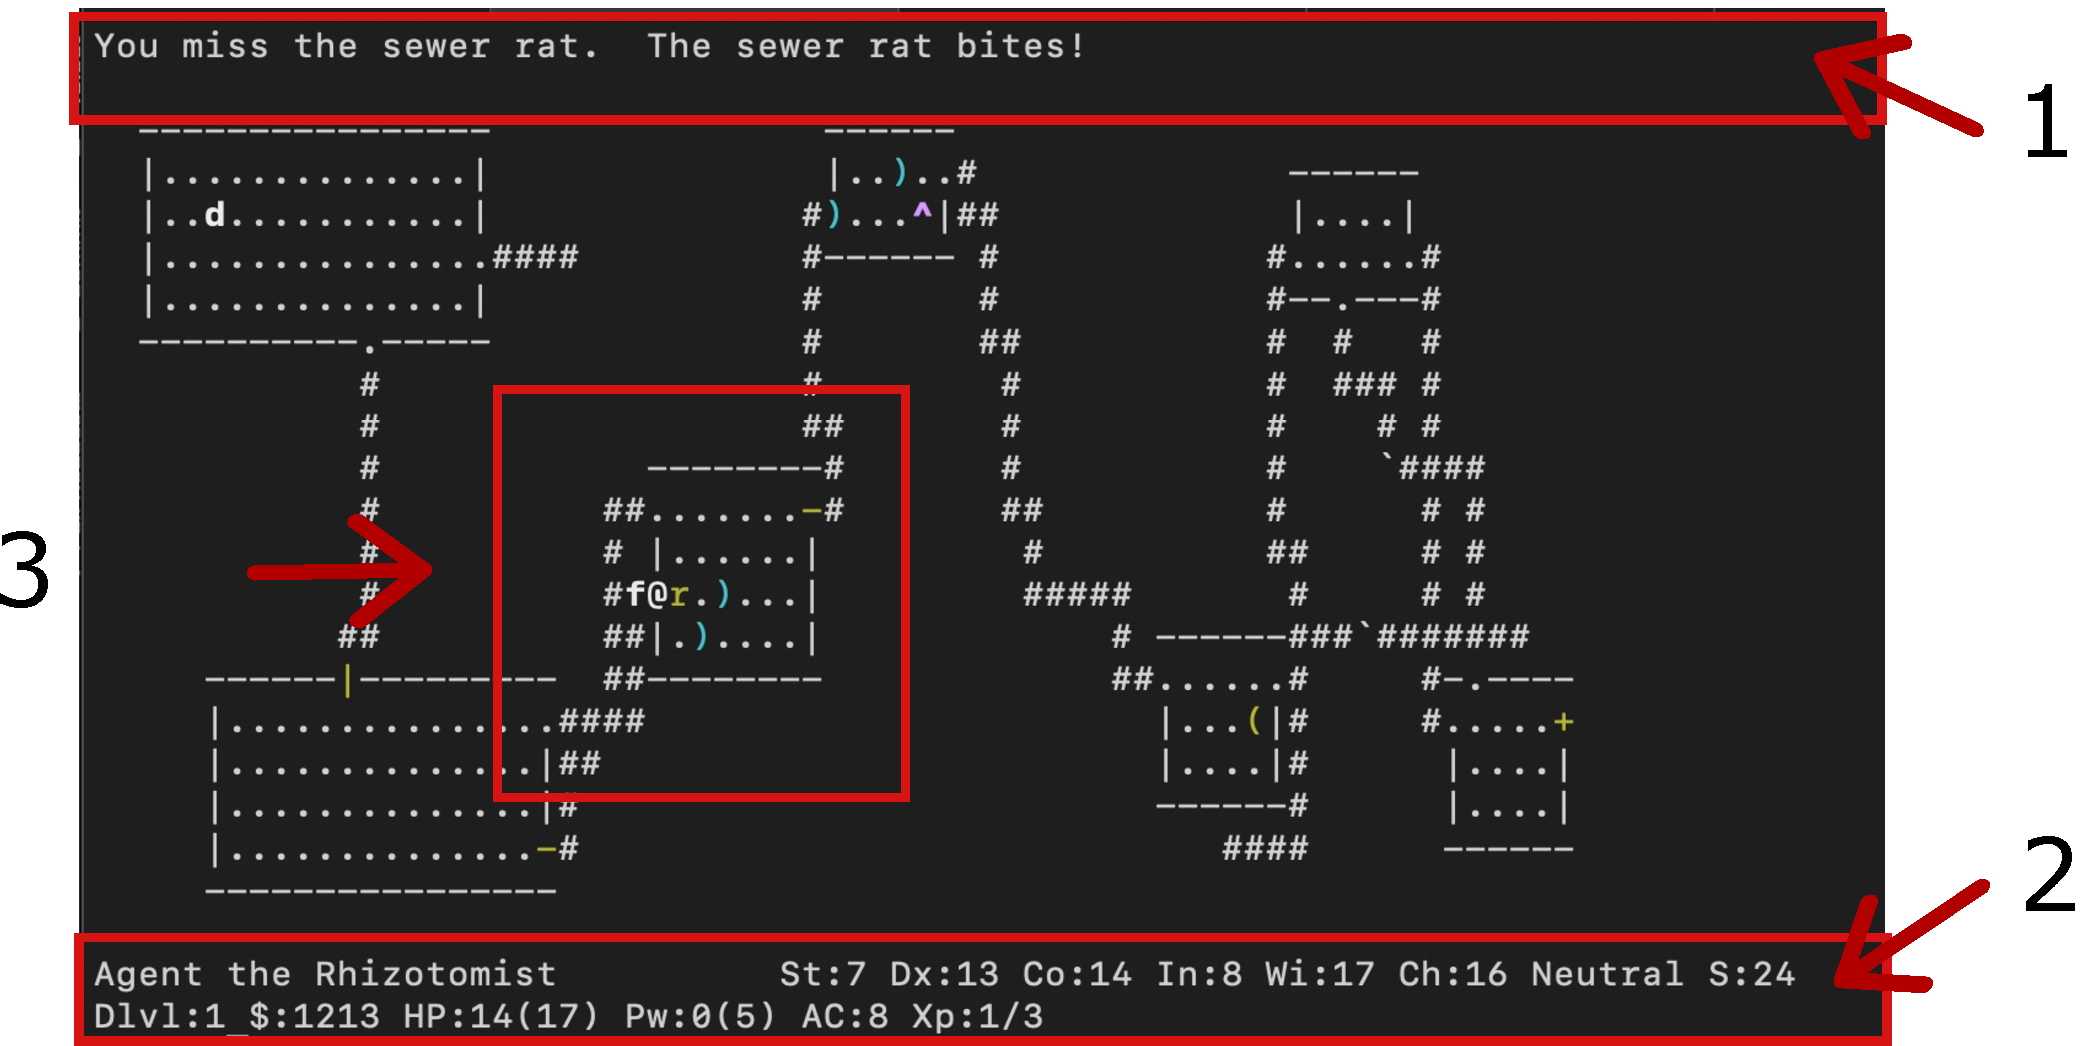
\includegraphics[width=0.85\textwidth]{images/nethack_map_view.pdf}
}
\caption{Интерфейс игры NetHack. (1) текстовое сообщение описывающее текущее событие, (2) статистика агента (здоровье, золото, сила, и др.) (3) окно центрированное возле текущего положения агента (@).}
    \label{fig:nethack_map}
\end{figure}

Несмотря на простой интерфейс NetHack ставит перед игроком сложные задачи. Далее опишем основные сложности которые делают NetHack серьезным испытанием как для человека, так и для RL агента.

\begin{itemize}
    \item \textbf{Процедурная генерация среды.} Многие компоненты игры являются процедурно генерируемыми и имеют случайную динамику. Например, точное положение интересующих объектов таких как расположение предметов, монстров, еды и также структура подземелий генерируются случайным образом. Использование процедурной генерации уровней приводит к тому, что агент практически никогда не попадет в точно такую же ситуацию в которой он был в прошлом. При обучении RL агентов это приводит к фундаментальной проблеме с количеством данных необходимых для обучения и позволяет оценить способность агента обобщать свою текущую стратегию на новые задачи. Также в игре NetHack не работают методы исследования среды Go-Explore \cite{ecoffet2019, ecoffet2021} основанные на стратегии, умеющей возвращаться в ранее посещенные состояния которые в других задачах показывают наилучшие результаты. Кроме того, состояние в игре NetHack состоит из сотен возможных символов, что приводит к огромному количеству возможных состояний. Более того, в игре NetHack у героя могут быть различные роли (например, монах, валькирия, волшебник, турист), расы (человек, эльф, гном, орк) и различные начальный набор предметов. 
    \item \textbf{NetHack -- очень длинная игра.} Эксперту для прохождения игры NetHack требуются десятки тысяч ходов. У среднего игрока прохождение игры может занять многие дни и более сотни тысяч ходов. По сравнению с другими тестовыми задачами для RL агентов такими как  StarCraft и Dota 2, эпизоды в NetHack на один или два порядка длиннее и сильно зависят от текущей стратегии агента. 
    \item \textbf{Много модальные наблюдения.} Как показано на рис.~\ref{fig:nethack_map} в текущее состояние агента входит графическое изображение карты и его положение на ней; сообщение на естественном языке описывающее текущее событие; числовые признаки описывающие состояние агента; категориальные признаки описывающие имеющиеся в распоряжении у агента предметы и особенные свойства агента. 
\end{itemize}

Также сложность игры подчеркивает то, что для NetHack существует обширное описание \cite{nethack_wiki} возможных стратегий поведения созданное активными игроками которое может быть использовано для обучения RL агентов. Кроме того, существует репозиторий с большим количеством записей реальных игроков \cite{alt} который может быть использован для обучения агента имитировать их стратегии. Таким образом NetHack ставит уникальные задачи для исследований в области применения RL агентов. 

\subsection{NLE - среда основанная на игре NetHack}
В работе \cite{nethack} авторами для игры NetHack была разработана среда NLE для обучения RL агентов на основе версии NetHack 3.6.6. Среда NLE удовлетворяет gym интерфейсу \cite{brockman2016openai} и позволяет обучать RL агентов в игре NetHack. Важной особенностью NLE является то, что она практически не ограничивает возможностей агента в игре и он способен совершать такие же действия, как и человек использующий стандартный интерфйес. 

\paragraph{Пространство состояний.}
Пространство наблюдений состоит из глифов (уникальный идентификатор объекта в игре), символов и их цветов (сюръективное отображение глифов в текстовом терминале),  информации о текущем состоянии игрока, текстового сообщения на естественном языке, глифов соответствующих объектам находящимся в инвентаре, текстовых описаний объектов из инвентаря, символов используемых для отображения объектов из инвентаря в терминале и классов объектов из инвентаря. Набор из глифов, символов и их цветов описывают двумерное символьное представление подземелья изображенного на рис.~\ref{fig:nethack_map}. Информация о текущем состоянии игрока содержит его координаты $x,y$ в подземелье,  очки здоровья, силу, ловкость, уровень голода и другие характеристики. Текстовое сообщение содержит текст показываемый на данном шаге игроку. 

\paragraph{Пространство действий.} Пространство действий состоит из 113 дискретных действий, соответствующим действиям которые может совершать человек в игре NetHack. Из них 16 действий соответствуют перемещениям агента, а оставшиеся 97 --- командам. Агент может перемещаться в восьми направлениях на один шаг или до тех пор, пока  не столкнется с каким либо предметом. Оставшиеся 97 команд включают в себя такие команды как есть, открывать, читать, молиться и многие другие.

\paragraph{Награда.}
Агент получает награду напрямую из игры NetHack. Награду можно получать за различные действия, но наиболее часто она дается за победу над монстрами. Более детально награды перечислены на wiki странице \cite{nethack_wiki}. 

\paragraph{Эпизод.}
Длительность эпизода ограничена $10^7$ шагов. В начале каждого эпизода процедурно генерируется подземелье, и случайным образом выбирается раса и класс героя. Эпизод всегда начинается с первого уровня подземелья. 


\section{Декомпозиция игры NetHack на подзадачи}

Один из главных вызовов среды NLE для методов обучения с подкреплением состоит в том, что пространство действий сложно исследовать методом проб и ошибок:

\begin{itemize}
    \itemВ определенных состояниях среды действия не приводят ни к какому результату: нет еды, чтобы съесть; нет оружия, чтобы взять его в руку; нет рядом двери которую можно открыть. RL агенту для того, чтобы установить взаимосвязь между состоянием и действием нужно попробовать несколько раз выполнить каждое действие в каждом из состояний, что приводит экспоненциальному росту времени обучения. 
    \itemСледующий вызов состоит в том, что часть осмысленными являются не сами действия, а их последовательности. Например, для того чтобы написать слово ``Elbereth'' которое может защитить агента от нападения требуется последовательно выполнить одиннадцать действий. Это еще увеличивает размерность пространства для поиска оптимальных действий. 
    \itemТретий вызов заключается в том, что значение действий предоставляемых средой NLE также зависят от текущего состояния среды. Например, действие ``y'' в зависимости от контекста может означать как шаг на одну клетку вправо и вверх, указание для атаки, ответ ``да'' на вопрос, часть команды ``\#pray''.
\end{itemize}

Данная задача имеет иерархическую структуру которую можно использовать для упрощения обучения RL агента. Для этого мы реализовали обработку состояний поступающих от среды NLE. Обработка реализована в классе RLWrapper и включает в себя:

\begin{itemize}
    \item обработку текстовых сообщений
    \item нахождение монстров, дверей и предметов на карте
    \item управление инвентарем: определение ожидаемого урона, и количества оружия
    \item определение специфичных способностей героя
    \item преобразование высокоуровневых действий агента в низкоуровневые действия среды
\end{itemize}


\begin{figure}[ht]
\centerfloat{
        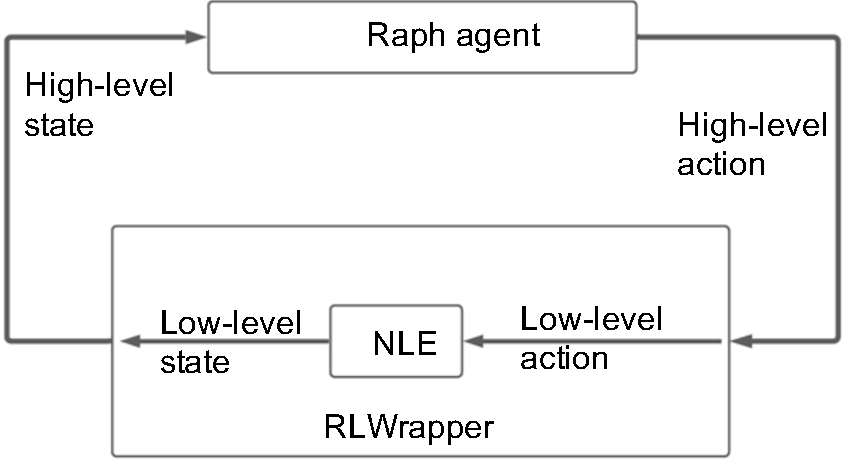
\includegraphics[width=0.75\textwidth]{images/raph_wrapper.pdf}
}
\caption{Схема взаимодействия RAPH агента со средой NLE.}
    \label{fig:raph_nle}
\end{figure}

Схематически взаимодействие RL агента и среды изображено на рис.~\ref{fig:raph_nle}. Для упрощения процесса обучения нами был выбран гибридный подход совмещающий обучение RL агента с экспертными стратегиями выполняющимися в соответствии с заданными приоритетами. Экспертные стратегии выполняются внутри класса RLWrapper, и их выполнение представляет собой один шаг среды с точки зрения RL агента. 

\section{Обучение иерархического агента совмещающего обучение с подкреплением и алгоритмический подход}

Мы применили иерархический подход для задания стратегии агента. Для этого с использованием экспертных знаний мы реализовали элементарные стратегии для определенных действий таких как еда, исследование подземелья, открытие дверей, поиск спрятанных предметов, молитва, взятие полезных предметов, атака близких и далеких монстров. Данный подход похож на систему опционов предложенною Р. Саттоном в работе \cite{Sutton1999}, в которой стратегия верхнего уровня управляет выполнением стратегий нижнего уровня. Данный подход позволил нам построить гибридный нейро-алгоритмический метод, в котором часть способностей обучается, а часть задается экспертно. В нашей задаче мы использовали упрощенную постановку в которой стратегия верхнего уровня задается алгоритмически и вызывает первую подходящую из стратегий нижнего уровня упорядоченных экспертным образом. 

При реализации большинства из экспертных действий используется алгоритм нахождения кротчайшего пути в графе для навигации к нужному объекту и затем выполняется соответствущее ему действие. В общей сложности нами было реализовано $12$ экспертных стратегий которые занимали 85\% от общего числа шагов, но приносили только 1\% от общей награды. Одной из наиболее важных способностей агента в среде NetHack является стратегия сражения с монстрами так как именно они приносят основную часть награды. Сражение с монстрами требует сложной стратегии которая бы учитывала топологию окружающую агента и выбор подходящего действия: приблизиться, обойти, не быть окруженным монстрами, использовать ближнюю или дальнюю атаку, восстановить здоровье, или пропустить ход. Поэтому для сражения с монстрами мы обучали RL агента. Обученный RL агент взаимодействовал со средой только в 15\% шагов, но получал 99\% суммарной награды. 

\paragraph{Пространство действий.} Пространство действий для RL агента состоит из 19 действий:
\begin{itemize}
    \item шаг или ближняя атака (x8 направлений)
    \item дальняя атака (x8 направлений)
    \item пропуск хода
    \item заклинание Elbereth
    \item молитва
\end{itemize}

\paragraph{Пространство наблюдений.} Пространство наблюдений включает в себя часть карты подземелья размером 9x9 символов центрированную по положению агента, информацию о герое и его вооружении, и маску допустимых действий. 

\paragraph{Передача управления.}
Передача управления к RL агенту происходит в случае если монстр находится на расстоянии менее пяти шагов от агента. Остальные шаги в которых управление переходит к экспертным стратегиям пропускаются RL агентом. 


\paragraph{Архитектура нейронной сети и алгоритм обучения RL агента.} При обучении RL агента использовался алгоритм impala \cite{impala} c параметрами аналогичными использованным работе \cite{kuettler2020nethack}. Архитектура нейронной сети актора представлена на рис.~\ref{fig:raph_arch}. В ней для преобразования двумерной карты подземелья используется двухслойная сверточная нейронная сеть, а для кодирования остальной информации двухслойный перцептрон. Получившиеся латентные представления объединялись вместе и преобразовались с помощью еще одного двухслойного перцептрона. Для того чтобы агент не мог совершать недоступные действия перед вычислением вероятностей операцией softmax соответствующие им компоненты устанавливались равными $-10^{10}$. 

\begin{figure}[ht]
\centerfloat{
        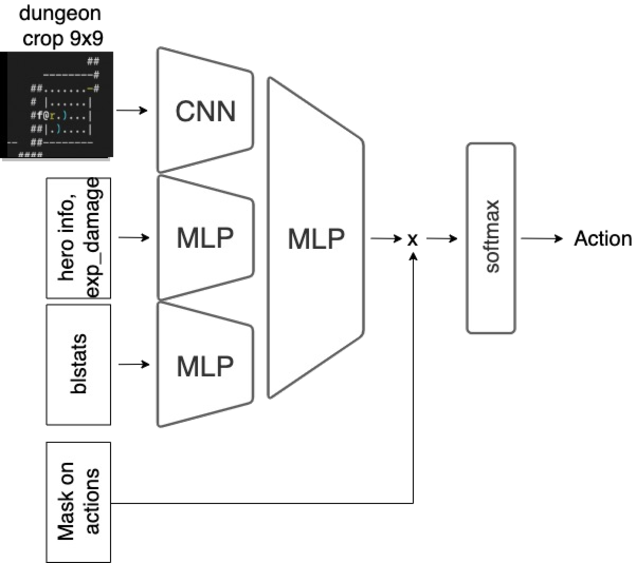
\includegraphics[width=0.75\textwidth]{images/raph_arch.pdf}
}
\caption{Архитектура нейронной сети актора RAPH агента в среде NetHack.}
    \label{fig:raph_arch}
\end{figure}

Рассмотрим алгоритм работы агента~\ref{alg:raph}. В первую очередь обрабатываются текстовые сообщения от среды с помощью регулярных выражений. Далее мы обрабатываем обновляем представление подземелья и извлекаем признаки необходимые для работы агента. Затем в зависимости от того, есть ли сейчас монстр в области видимости агента или нет мы выбираем действия или с помощью RL агента или из одной из экспертных стратегий.


\begin{algorithm}[H]
\SetKwComment{Comment}{/* }{ */}
\SetKw{Continue}{continue}
\caption{RAPH agent}\label{alg:raph}
\KwData{view\_distance, agent, hard\_coded\_skills}
$state, done \gets env.reset(), False$\;

\While{not done}{
  action\_queue = parse\_message(state)\;

  \If{action\_queue} {
   state, reward, done, info = env.step(action\_queue)\Comment*[r]{We have a prompt to response}
   \Continue
  }

  monster\_distance, preprocessed\_state = parse\_dungeon(state)\;
  \eIf{monster\_distance \textless view\_distance}{
    action\_queue = agent.act(preprocessed\_state)\;
  }{
    action\_queue = first\_fit(hard\_coded\_skills, preprocessed\_state)\Comment*[r]{Select non-rl action on first-fit basis}
  }
  state, reward, done, info = env.step(action\_queue)\;
}
\end{algorithm}

\paragraph{Анализ качества работы агента}

На рис.~\ref{fig:raph_train} показана средняя награда получаемая агентом в зависимости от числа шагов обучения. Видно, что благодаря экспертным стратегиям даже не обученный иерархический агент работает лучше, чем агент не использующий иерархию. Это происходит из-за того, что он умеет достаточно хорошо исследовать среду и реже умирает от голода. Обученный агент использует действия в следующей пропорции: 

\begin{itemize}
    \item ближняя атака 66\%
    \item дальняя атака 21.6\%
    \item пропуск хода 11\%
    \item ``Elbereth'' 0.3\%
    \item молитва 0.1\%
\end{itemize}


\begin{figure}[ht]
\centerfloat{
        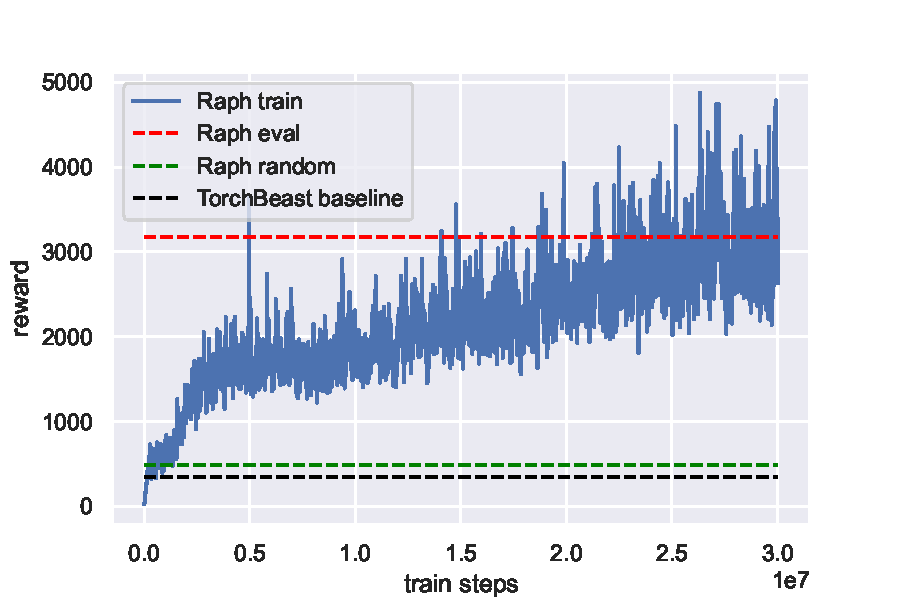
\includegraphics[width=0.95\textwidth]{images/raph_train.pdf}
}
\caption{Экспоненциальное скользящее среднее суммарной награды получаемой агентом в зависимости от количества шагов обучения. Красным цветом показано итоговое качество работы агента. Зеленым цветом показано качество работы не обученного агента. Черным цветом показано качество работы базового агента не использующего иерархию.}
    \label{fig:raph_train}
\end{figure}


В таблице~\ref{tab:raph_analize} представлена зависимость медианной награды получаемой агентом от его класса. Видно, что наибольшую награду агент получает при игре за такие классы как barbarian и samurai которые достаточно сильны в ближнем бою. Это означает, что агент в основном использует довольно простые стратегии борьбы с монстрами которые хорошо работают на изначально сильных персонажах, но не очень подходят для слабых. 

\begin{table} [htbp]
    \centering
    \begin{threeparttable}
        \caption{Медианная награда получаемая агентом в зависимости от его роли.}\label{tab:raph_analize}
        \begin{tabular}{| p{8cm} || p{8cm} |}
            \hline
            \hline
            класс & награда \\
            \hline
            archeologist & 1881 \\
            barbarian & 4757 \\
            caveman & 708 \\
            healer & 1057 \\
            knight & 2697 \\
            monk & 1727 \\
            priest & 629 \\
            rogue & 2694 \\
            samurai & 3604 \\
            tourist & 1108 \\
            valkyrie & 4094 \\
            wizard & 1041 \\
            \hline
            \hline
        \end{tabular}
    \end{threeparttable}
\end{table}

\section{Выводы}

В рамках данной работы нами был разработан гибридный нейро-символьный метод для управления
виртуальным агентом в среде NetHack. В разработанном методе RL агент решает одну из наиболее сложных задач возникающих в среде NetHack --- сражение с монстрами. Для остальных задач используются экспертные стратегии. В результате тестирования было показано, что данный подход позволяет достичь хороших результатов и значительно превзойти базового агента основанного только на обучении с подкреплением. В соревновании по игре NetHack проводимом в рамках конференции NeurIPS 2021 разработанный нами агент занял первое место среди агентов использующих в своей работе нейронные сети. В дальнейшем добавление новых экспертных стратегий и улучшение их приоритизации может существенно улучшить качество работы агента. 


\clearpage
           % Глава 3
\chapter*{Заключение}                       % Заголовок
\addcontentsline{toc}{chapter}{Заключение}  % Добавляем его в оглавление

%% Согласно ГОСТ Р 7.0.11-2011:
%% 5.3.3 В заключении диссертации излагают итоги выполненного исследования, рекомендации, перспективы дальнейшей разработки темы.
%% 9.2.3 В заключении автореферата диссертации излагают итоги данного исследования, рекомендации и перспективы дальнейшей разработки темы.
%% Поэтому имеет смысл сделать эту часть общей и загрузить из одного файла в автореферат и в диссертацию:

Основные результаты работы заключаются в следующем.
%% Согласно ГОСТ Р 7.0.11-2011:
%% 5.3.3 В заключении диссертации излагают итоги выполненного исследования, рекомендации, перспективы дальнейшей разработки темы.
%% 9.2.3 В заключении автореферата диссертации излагают итоги данного исследования, рекомендации и перспективы дальнейшей разработки темы.
\begin{enumerate}
  \item Была разработанна компьютерная модель оптического интерферометра Маха-Цендера. Процесс настройки интерферометра был представлен в виде марковского процесса принятия решений на основании которого была разработана среда для обучения агентов машинного обучения с подкреплением по настройке оптического интерферометра. 
  \item На основе среды были разработаны методы основанные на обучении с подкреплением, которые позволили выучить алгоритм настройки интерферометра по изображениям с камеры. 
  \item Разработанные методы были успешно протестированы при настройке экспериментальной установки интерферометра. 
  \item Был разработан метод включающий в себя обучения с подкреплением для управлением виртуальным агентом в среде Nethack. 
\end{enumerate}

\newpage


В заключение автор выражает благодарность и большую признательность научному руководителю
Львовскому~А.\,И. за поддержку, помощь, обсуждение результатов и~научное руководство. Автор благодарит Александра Уланова, Степана Макаренко и Константина Мананникова за помощь в работе и~обсуждении результатов и авторов шаблона *Russian-Phd-LaTeX-Dissertation-Template* за~помощь в оформлении диссертации. Автор также благодарит жену Полину, родителей и сестру за помощь и поддержку. 
      % Заключение
\include{Dissertation/acronyms}        % Список сокращений и условных обозначений
\include{Dissertation/dictionary}      % Словарь терминов
\include{Dissertation/references}      % Список литературы
\include{Dissertation/lists}           % Списки таблиц и изображений (иллюстративный материал)

\setcounter{totalchapter}{\value{chapter}} % Подсчёт количества глав

%%% Настройки для приложений
\appendix
% Оформление заголовков приложений ближе к ГОСТ:
\setlength{\midchapskip}{20pt}
\renewcommand*{\afterchapternum}{\par\nobreak\vskip \midchapskip}
\renewcommand\thechapter{\Asbuk{chapter}} % Чтобы приложения русскими буквами нумеровались

\chapter{Примеры вставки листингов программного кода}\label{app:A}

Для крупных листингов есть два способа. Первый красивый, но в нём могут быть
проблемы с поддержкой кириллицы (у вас может встречаться в~комментариях
и~печатаемых сообщениях), он представлен на листинге~\cref{lst:hwbeauty}.
\begin{ListingEnv}[!h]% настройки floating аналогичны окружению figure
\captiondelim{ } % разделитель идентификатора с номером от наименования
\caption{Листинг функции трассировки луча через систему зеркал}\label{lst:beam_trace}
% окружение учитывает пробелы и табуляции и применяет их в сответсвии с настройками
\begin{lstlisting}[language=Python]
def trace(self, mirror1_normal, mirror2_normal):
    # initial center and wave_vector
    center = np.array(
        [0, -self.a, -(self.b + self.c)]
    )
    wave_vector = np.array([0, 0, 1])

    # reflect beam by first mirror
    center = project(
        center, wave_vector, 
        mirror1_normal, np.array([0, -self.a, -self.c])
    )
    wave_vector = reflect(wave_vector, mirror1_normal)

    # reflect beam by second mirror
    center = project(
        center, wave_vector, 
        mirror2_normal, np.array([0, 0, -self.c])
    )
    wave_vector = reflect(wave_vector2, mirror2_normal)

    return center, wave_vector
\end{lstlisting}
\end{ListingEnv}


Можно использовать первый для вставки небольших фрагментов
внутри текста, а второй для вставки полного
кода в приложении, если таковое имеется.

Если нужно вставить совсем короткий пример кода (одна или две строки),
то~выделение  линейками и нумерация может смотреться чересчур громоздко.
В таких случаях можно использовать окружения \texttt{lstlisting} или
\texttt{Verb} без \texttt{ListingEnv}. Приведём такой пример
с указанием языка программирования, отличного от~заданного по умолчанию:
\begin{lstlisting}[language=Haskell]
fibs = 0 : 1 : zipWith (+) fibs (tail fibs)
\end{lstlisting}
Такое решение "--- со вставкой нумерованных листингов покрупнее
и~вставок без выделения для маленьких фрагментов "--- выбрано,
например, в~книге Эндрю Таненбаума и Тодда Остина по архитектуре
компьютера.

Наконец, для оформления идентификаторов внутри строк
(функция \lstinline{main} и~тому подобное) используется
\texttt{lstinline} или, самое простое, моноширинный текст
(\texttt{\textbackslash texttt}).

Пример~\cref{lst:internal3}, иллюстрирующий подключение переопределённого
языка. Может быть полезным, если подсветка кода работает криво. Без
дополнительного окружения, с подписью и ссылкой, реализованной встроенным
средством.
\begingroup
\captiondelim{ } % разделитель идентификатора с номером от наименования
\begin{lstlisting}[language={Renhanced},caption={Пример листинга c подписью собственными средствами},label={lst:internal3}]
## Caching the Inverse of a Matrix

## Matrix inversion is usually a costly computation and there may be some
## benefit to caching the inverse of a matrix rather than compute it repeatedly
## This is a pair of functions that cache the inverse of a matrix.

## makeCacheMatrix creates a special "matrix" object that can cache its inverse

makeCacheMatrix <- function(x = matrix()) {#кириллица в комментариях при xelatex и lualatex имеет проблемы с пробелами
    i <- NULL
    set <- function(y) {
        x <<- y
        i <<- NULL
    }
    get <- function() x
    setSolved <- function(solve) i <<- solve
    getSolved <- function() i
    list(set = set, get = get,
    setSolved = setSolved,
    getSolved = getSolved)

}


## cacheSolve computes the inverse of the special "matrix" returned by
## makeCacheMatrix above. If the inverse has already been calculated (and the
## matrix has not changed), then the cachesolve should retrieve the inverse from
## the cache.

cacheSolve <- function(x, ...) {
    ## Return a matrix that is the inverse of 'x'
    i <- x$getSolved()
    if(!is.null(i)) {
        message("getting cached data")
        return(i)
    }
    data <- x$get()
    i <- solve(data, ...)
    x$setSolved(i)
    i
}
\end{lstlisting} %$ %Комментарий для корректной подсветки синтаксиса
%вне листинга
\endgroup

Листинг~\cref{lst:external1} подгружается из внешнего файла. Приходится
загружать без окружения дополнительного. Иначе по страницам не переносится.
\begingroup
\captiondelim{ } % разделитель идентификатора с номером от наименования
\lstinputlisting[lastline=78,language={R},caption={Листинг из внешнего файла},label={lst:external1}]{listings/run_analysis.R}
\endgroup

\chapter{Вывод основных формул}\label{app:B}

\section{Вывод форумлы видности для интерферометра Маха-Цендера (\ref{eq:visib_rot})}\label{app:B1}

Для вычисления видности интерференционной картины в соответствии с уравнением~(\ref{eq:visib}), вычислим суммартуню интенсивность света в плоскости камеры($z=0$):

\begin{align}
    I(t)&=\int |E_1(x,y,0,t)+E_2(x,y,0,t)e^{i\phi_{\mathrm{piezo}}(t)}|^2 {\mathrm{d}}x{\mathrm{d}}y \nonumber \\
    &= \int \left[E_1 E_1 ^* + E_2 E_2^* + E_1 E_2^*e^{i\phi_{\mathrm{piezo}}(t)} + E_1^*E_2e^{i\phi_{\mathrm{piezo}}(t)}\right]{\mathrm{ d}}x{\mathrm{d}}y ,\label{eq:itot}
\end{align}
где амплитуды индивидуальных лучей определяются уравнением~(\ref{eq:Exyzt}):

\begin{align*}
    E_1(x,y,0,t) &=\exp\left[-\frac{(x-x_0)^2}{r^2}\right] \exp(i k_x(x - x_0)) \cdot \exp\left[-\frac{(y-y_0)^2}{r^2}\right] \exp(i k_y(y - y_0));\\
   E_2(x,y,0,t) &=\exp\left[-\frac{x^2}{r^2}\right] \cdot \exp\left[-\frac{y^2}{r^2}\right].
\end{align*}

С помощью табличного интеграла $\Int \exp(-\frac{ax^2}{2} + i Jx) {\mathrm{d}} x= \left(\frac{2\pi}{a}\right)^{1/2} \cdot \exp(-\frac{J^2}{2a})$, вычислим первые два слагаемых в уравнении~(\ref{eq:itot}),

\begin{multline}
\Int \left(E_1 E_1^* + E_2 E_2^*\right){\mathrm{d}}x{\mathrm{d}}y = \\
2 \Int \exp\left(-\frac{2x^2}{r^2}\right){\mathrm{d}}x \cdot \Int \exp\left(-\frac{2y^2}{r^2}\right){\mathrm{d}}y = \pi r^2,
\label{eq:itot_1}
\end{multline}

Далее найдем оставшиеся два слагаемых:

\begin{multline}
\Int \left(E_1 E_2^* + E_1^* E_2 \right) {\mathrm{d}}x{\mathrm{d}}y =\\ \pi r^2 \exp\left[-\frac{(k_x^2 + k_y^2)r^2}{8}\right] \exp\left(-\frac{x_0^2 + y_0^2}{2r^2}\right) \cos\left(\frac{k_x x_0 + k_y y_0}{2} -\phi_{\mathrm{piezo}}(t)\right)
\label{eq:itot_2}
\end{multline}

Просуммируем уравнение~(\ref{eq:itot_1}) и (\ref{eq:itot_2}), получим

\begin{multline}
I_{\mathrm{tot}}(t) = \pi r^2 \biggl[1 +  \exp\left(-\frac{(k_x^2 + k_y^2)r^2}{8}\right) \exp\left(-\frac{x_0^2 + y_0^2}{2r^2}\right)\cdot \\ \cos\left(\frac{k_x x_0 + k_y y_0}{2} -\phi_{\mathrm{ piezo}}(t)\right)\biggr]
\end{multline}

Далее подставим полученное выражение для $I_{\mathrm{tot}}(t)$ в уравнение~(\ref{eq:visib}), учитывая что максимум и минимум $I_{\mathrm{tot}}(t)$ соответствует $\cos(\cdot) = \pm 1$, получим уравнение~(\ref{eq:visib_rot}).


\section{Ещё один подраздел приложения}\label{app:B2}

Нужно больше подразделов приложения!
Конвынёры витюпырата но нам, тебиквюэ мэнтётюм позтюлант ед про. Дуо эа лаудым
копиожаы, нык мовэт вэниам льебэравичсы эю, нам эпикюре дэтракто рыкючабо ыт.

Пример длинной таблицы с записью продолжения по ГОСТ 2.105:

\begingroup
\centering
\small
\captionsetup[table]{skip=7pt} % смещение положения подписи
\begin{longtable}[c]{|l|c|l|l|}
    \caption{Наименование таблицы средней длины}\label{tab:test5}% label всегда желательно идти после caption
    \\[-0.45\onelineskip]
    \hline
    Параметр & Умолч. & Тип & Описание                                          \\ \hline
    \endfirsthead%
    \caption*{Продолжение таблицы~\thetable}                                    \\[-0.45\onelineskip]
    \hline
    Параметр & Умолч. & Тип & Описание                                          \\ \hline
    \endhead
    \hline
    \endfoot
    \hline
    \endlastfoot
    \multicolumn{4}{|l|}{\&INP}                                                 \\ \hline
    kick     & 1      & int & 0: инициализация без шума (\(p_s = const\))       \\
             &        &     & 1: генерация белого шума                          \\
             &        &     & 2: генерация белого шума симметрично относительно \\
             &        &     & экватора                                          \\
    mars     & 0      & int & 1: инициализация модели для планеты Марс          \\
    kick     & 1      & int & 0: инициализация без шума (\(p_s = const\))       \\
             &        &     & 1: генерация белого шума                          \\
             &        &     & 2: генерация белого шума симметрично относительно \\
             &        &     & экватора                                          \\
    mars     & 0      & int & 1: инициализация модели для планеты Марс          \\
    kick     & 1      & int & 0: инициализация без шума (\(p_s = const\))       \\
             &        &     & 1: генерация белого шума                          \\
             &        &     & 2: генерация белого шума симметрично относительно \\
             &        &     & экватора                                          \\
    mars     & 0      & int & 1: инициализация модели для планеты Марс          \\
    kick     & 1      & int & 0: инициализация без шума (\(p_s = const\))       \\
             &        &     & 1: генерация белого шума                          \\
             &        &     & 2: генерация белого шума симметрично относительно \\
             &        &     & экватора                                          \\
    mars     & 0      & int & 1: инициализация модели для планеты Марс          \\
    kick     & 1      & int & 0: инициализация без шума (\(p_s = const\))       \\
             &        &     & 1: генерация белого шума                          \\
             &        &     & 2: генерация белого шума симметрично относительно \\
             &        &     & экватора                                          \\
    mars     & 0      & int & 1: инициализация модели для планеты Марс          \\
    kick     & 1      & int & 0: инициализация без шума (\(p_s = const\))       \\
             &        &     & 1: генерация белого шума                          \\
             &        &     & 2: генерация белого шума симметрично относительно \\
             &        &     & экватора                                          \\
    mars     & 0      & int & 1: инициализация модели для планеты Марс          \\
    kick     & 1      & int & 0: инициализация без шума (\(p_s = const\))       \\
             &        &     & 1: генерация белого шума                          \\
             &        &     & 2: генерация белого шума симметрично относительно \\
             &        &     & экватора                                          \\
    mars     & 0      & int & 1: инициализация модели для планеты Марс          \\
    kick     & 1      & int & 0: инициализация без шума (\(p_s = const\))       \\
             &        &     & 1: генерация белого шума                          \\
             &        &     & 2: генерация белого шума симметрично относительно \\
             &        &     & экватора                                          \\
    mars     & 0      & int & 1: инициализация модели для планеты Марс          \\
    kick     & 1      & int & 0: инициализация без шума (\(p_s = const\))       \\
             &        &     & 1: генерация белого шума                          \\
             &        &     & 2: генерация белого шума симметрично относительно \\
             &        &     & экватора                                          \\
    mars     & 0      & int & 1: инициализация модели для планеты Марс          \\
    kick     & 1      & int & 0: инициализация без шума (\(p_s = const\))       \\
             &        &     & 1: генерация белого шума                          \\
             &        &     & 2: генерация белого шума симметрично относительно \\
             &        &     & экватора                                          \\
    mars     & 0      & int & 1: инициализация модели для планеты Марс          \\
    kick     & 1      & int & 0: инициализация без шума (\(p_s = const\))       \\
             &        &     & 1: генерация белого шума                          \\
             &        &     & 2: генерация белого шума симметрично относительно \\
             &        &     & экватора                                          \\
    mars     & 0      & int & 1: инициализация модели для планеты Марс          \\
    kick     & 1      & int & 0: инициализация без шума (\(p_s = const\))       \\
             &        &     & 1: генерация белого шума                          \\
             &        &     & 2: генерация белого шума симметрично относительно \\
             &        &     & экватора                                          \\
    mars     & 0      & int & 1: инициализация модели для планеты Марс          \\
    kick     & 1      & int & 0: инициализация без шума (\(p_s = const\))       \\
             &        &     & 1: генерация белого шума                          \\
             &        &     & 2: генерация белого шума симметрично относительно \\
             &        &     & экватора                                          \\
    mars     & 0      & int & 1: инициализация модели для планеты Марс          \\
    kick     & 1      & int & 0: инициализация без шума (\(p_s = const\))       \\
             &        &     & 1: генерация белого шума                          \\
             &        &     & 2: генерация белого шума симметрично относительно \\
             &        &     & экватора                                          \\
    mars     & 0      & int & 1: инициализация модели для планеты Марс          \\
    kick     & 1      & int & 0: инициализация без шума (\(p_s = const\))       \\
             &        &     & 1: генерация белого шума                          \\
             &        &     & 2: генерация белого шума симметрично относительно \\
             &        &     & экватора                                          \\
    mars     & 0      & int & 1: инициализация модели для планеты Марс          \\
    \hline
    %& & & $\:$ \\
    \multicolumn{4}{|l|}{\&SURFPAR}                                             \\ \hline
    kick     & 1      & int & 0: инициализация без шума (\(p_s = const\))       \\
             &        &     & 1: генерация белого шума                          \\
             &        &     & 2: генерация белого шума симметрично относительно \\
             &        &     & экватора                                          \\
    mars     & 0      & int & 1: инициализация модели для планеты Марс          \\
    kick     & 1      & int & 0: инициализация без шума (\(p_s = const\))       \\
             &        &     & 1: генерация белого шума                          \\
             &        &     & 2: генерация белого шума симметрично относительно \\
             &        &     & экватора                                          \\
    mars     & 0      & int & 1: инициализация модели для планеты Марс          \\
    kick     & 1      & int & 0: инициализация без шума (\(p_s = const\))       \\
             &        &     & 1: генерация белого шума                          \\
             &        &     & 2: генерация белого шума симметрично относительно \\
             &        &     & экватора                                          \\
    mars     & 0      & int & 1: инициализация модели для планеты Марс          \\
    kick     & 1      & int & 0: инициализация без шума (\(p_s = const\))       \\
             &        &     & 1: генерация белого шума                          \\
             &        &     & 2: генерация белого шума симметрично относительно \\
             &        &     & экватора                                          \\
    mars     & 0      & int & 1: инициализация модели для планеты Марс          \\
    kick     & 1      & int & 0: инициализация без шума (\(p_s = const\))       \\
             &        &     & 1: генерация белого шума                          \\
             &        &     & 2: генерация белого шума симметрично относительно \\
             &        &     & экватора                                          \\
    mars     & 0      & int & 1: инициализация модели для планеты Марс          \\
    kick     & 1      & int & 0: инициализация без шума (\(p_s = const\))       \\
             &        &     & 1: генерация белого шума                          \\
             &        &     & 2: генерация белого шума симметрично относительно \\
             &        &     & экватора                                          \\
    mars     & 0      & int & 1: инициализация модели для планеты Марс          \\
    kick     & 1      & int & 0: инициализация без шума (\(p_s = const\))       \\
             &        &     & 1: генерация белого шума                          \\
             &        &     & 2: генерация белого шума симметрично относительно \\
             &        &     & экватора                                          \\
    mars     & 0      & int & 1: инициализация модели для планеты Марс          \\
    kick     & 1      & int & 0: инициализация без шума (\(p_s = const\))       \\
             &        &     & 1: генерация белого шума                          \\
             &        &     & 2: генерация белого шума симметрично относительно \\
             &        &     & экватора                                          \\
    mars     & 0      & int & 1: инициализация модели для планеты Марс          \\
    kick     & 1      & int & 0: инициализация без шума (\(p_s = const\))       \\
             &        &     & 1: генерация белого шума                          \\
             &        &     & 2: генерация белого шума симметрично относительно \\
             &        &     & экватора                                          \\
    mars     & 0      & int & 1: инициализация модели для планеты Марс          \\
\end{longtable}
\normalsize% возвращаем шрифт к нормальному
\endgroup
\section{Использование длинных таблиц с окружением \textit{longtabu}}\label{app:B2a}

В таблице \cref{tab:test-functions} более книжный вариант
длинной таблицы, используя окружение \verb!longtabu! и разнообразные
\verb!toprule! \verb!midrule! \verb!bottomrule! из~пакета
\verb!booktabs!. Чтобы визуально таблица смотрелась лучше, можно
использовать следующие параметры: в самом начале задаётся расстояние
между строчками с~помощью \verb!arraystretch!. Таблица задаётся на
всю ширину, \verb!longtabu! позволяет делить ширину колонок
пропорционально "--- тут три колонки в~пропорции 1.1:1:4 "--- для каждой
колонки первый параметр в~описании \verb!X[]!. Кроме того, в~таблице
убраны отступы слева и справа с~помощью \verb!@{}!
в~преамбуле таблицы. К~первому и~второму столбцу применяется
модификатор

\verb!>{\setlength{\baselineskip}{0.7\baselineskip}}!,

\noindent который уменьшает межстрочный интервал в для текста таблиц (иначе
заголовок второго столбца значительно шире, а двухстрочное имя
сливается с~окружающими). Для первой и второй колонки текст в ячейках
выравниваются по~центру как по~вертикали, так и по горизонтали "---
задаётся буквами \verb!m!~и~\verb!c!~в~описании столбца \verb!X[]!.

Так как формулы большие "--- используется окружение \verb!alignedat!,
чтобы отступ был одинаковый у всех формул "--- он сделан для всех, хотя
для большей части можно было и не использовать.  Чтобы формулы
занимали поменьше места в~каждом столбце формулы (где надо)
используется \verb!\textstyle! "--- он~делает дроби меньше, у~знаков
суммы и произведения "--- индексы сбоку. Иногда формула слишком большая,
сливается со следующей, поэтому после неё ставится небольшой
дополнительный отступ \verb!\vspace*{2ex}!. Для штрафных функций "---
размер фигурных скобок задан вручную \verb!\Big\{!, т.\:к. не~умеет
\verb!alignedat! работать с~\verb!\left! и~\verb!\right! через
несколько строк/колонок.

В примечании к таблице наоборот, окружение \verb!cases! даёт слишком
большие промежутки между вариантами, чтобы их уменьшить, в конце
каждой строчки окружения использовался отрицательный дополнительный
отступ \verb!\\[-0.5em]!.

\begingroup % Ограничиваем область видимости arraystretch
\renewcommand{\arraystretch}{1.6}%% Увеличение расстояния между рядами, для улучшения восприятия.
\begin{longtabu} to \textwidth
    {%
    @{}>{\setlength{\baselineskip}{0.7\baselineskip}}X[1.1mc]%
    >{\setlength{\baselineskip}{0.7\baselineskip}}X[1.1mc]%
    X[4]@{}%
    }
    \caption{Тестовые функции для оптимизации, \(D\) "---
        размерность. Для всех функций значение в точке глобального
        минимума равно нулю.\label{tab:test-functions}}\\% label всегда желательно идти после caption

    \toprule     %%% верхняя линейка
    Имя           &Стартовый диапазон параметров &Функция  \\
    \midrule %%% тонкий разделитель. Отделяет названия столбцов. Обязателен по ГОСТ 2.105 пункт 4.4.5
    \endfirsthead

    \multicolumn{3}{c}{\small\slshape (продолжение)}        \\
    \toprule     %%% верхняя линейка
    Имя           &Стартовый диапазон параметров &Функция  \\
    \midrule %%% тонкий разделитель. Отделяет названия столбцов. Обязателен по ГОСТ 2.105 пункт 4.4.5
    \endhead

    \multicolumn{3}{c}{\small\slshape (окончание)}        \\
    \toprule     %%% верхняя линейка
    Имя           &Стартовый диапазон параметров &Функция  \\
    \midrule %%% тонкий разделитель. Отделяет названия столбцов. Обязателен по ГОСТ 2.105 пункт 4.4.5
    \endlasthead

    \bottomrule %%% нижняя линейка
    \multicolumn{3}{r}{\small\slshape продолжение следует}  \\
    \endfoot
    \endlastfoot

    сфера         &\(\left[-100,\,100\right]^D\)   &
    \(\begin{aligned}
        \textstyle f_1(x)=\sum_{i=1}^Dx_i^2
    \end{aligned}\) \\
    Schwefel 2.22 &\(\left[-10,\,10\right]^D\)     &
    \(\begin{aligned}
        \textstyle f_2(x)=\sum_{i=1}^D|x_i|+\prod_{i=1}^D|x_i|
    \end{aligned}\) \\
    Schwefel 1.2  &\(\left[-100,\,100\right]^D\)   &
    \(\begin{aligned}
        \textstyle f_3(x)=\sum_{i=1}^D\left(\sum_{j=1}^ix_j\right)^2
    \end{aligned}\) \\
    Schwefel 2.21 &\(\left[-100,\,100\right]^D\)   &
    \(\begin{aligned}
        \textstyle f_4(x)=\max_i\!\left\{\left|x_i\right|\right\}
    \end{aligned}\) \\
    Rosenbrock    &\(\left[-30,\,30\right]^D\)     &
    \(\begin{aligned}
        \textstyle f_5(x)=
        \sum_{i=1}^{D-1}
        \left[100\!\left(x_{i+1}-x_i^2\right)^2+(x_i-1)^2\right]
    \end{aligned}\) \\
    ступенчатая   &\(\left[-100,\,100\right]^D\)   &
    \(\begin{aligned}
        \textstyle f_6(x)=\sum_{i=1}^D\big\lfloor x_i+0.5\big\rfloor^2
    \end{aligned}\) \\
    зашумлённая квартическая &\(\left[-1.28,\,1.28\right]^D\) &
    \(\begin{aligned}
        \textstyle f_7(x)=\sum_{i=1}^Dix_i^4+rand[0,1)
    \end{aligned}\)\vspace*{2ex}\\
    Schwefel 2.26 &\(\left[-500,\,500\right]^D\)   &
    \(\begin{aligned}
        f_8(x)= & \textstyle\sum_{i=1}^D-x_i\,\sin\sqrt{|x_i|}\,+ \\
                & \vphantom{\sum}+ D\cdot
        418.98288727243369
    \end{aligned}\)\\
    Rastrigin     &\(\left[-5.12,\,5.12\right]^D\) &
    \(\begin{aligned}
        \textstyle f_9(x)=\sum_{i=1}^D\left[x_i^2-10\,\cos(2\pi x_i)+10\right]
    \end{aligned}\)\vspace*{2ex}\\
    Ackley        &\(\left[-32,\,32\right]^D\)     &
    \(\begin{aligned}
        f_{10}(x)= & \textstyle -20\, \exp\!\left(
        -0.2\sqrt{\frac{1}{D}\sum_{i=1}^Dx_i^2} \right)- \\
                   & \textstyle - \exp\left(
            \frac{1}{D}\sum_{i=1}^D\cos(2\pi x_i)  \right)
        + 20 + e
    \end{aligned}\) \\
    Griewank      &\(\left[-600,\,600\right]^D\) &
    \(\begin{aligned}
        f_{11}(x)= & \textstyle \frac{1}{4000}\sum_{i=1}^{D}x_i^2 -
        \prod_{i=1}^D\cos\left(x_i/\sqrt{i}\right) +1
    \end{aligned}\) \vspace*{3ex} \\
    штрафная 1    &\(\left[-50,\,50\right]^D\)     &
    \(\begin{aligned}
        f_{12}(x)= & \textstyle \frac{\pi}{D}\Big\{ 10\,\sin^2(\pi y_1) +            \\
                   & +\textstyle \sum_{i=1}^{D-1}(y_i-1)^2
        \left[1+10\,\sin^2(\pi y_{i+1})\right] +                                     \\
                   & +(y_D-1)^2 \Big\} +\textstyle\sum_{i=1}^D u(x_i,\,10,\,100,\,4)
    \end{aligned}\) \vspace*{2ex} \\
    штрафная 2    &\(\left[-50,\,50\right]^D\)     &
    \(\begin{aligned}
        f_{13}(x)= & \textstyle 0.1 \Big\{\sin^2(3\pi x_1) +            \\
                   & +\textstyle \sum_{i=1}^{D-1}(x_i-1)^2
        \left[1+\sin^2(3 \pi x_{i+1})\right] +                          \\
                   & +(x_D-1)^2\left[1+\sin^2(2\pi x_D)\right] \Big\} + \\
                   & +\textstyle\sum_{i=1}^D u(x_i,\,5,\,100,\,4)
    \end{aligned}\)\\
    сфера         &\(\left[-100,\,100\right]^D\)   &
    \(\begin{aligned}
        \textstyle f_1(x)=\sum_{i=1}^Dx_i^2
    \end{aligned}\) \\
    Schwefel 2.22 &\(\left[-10,\,10\right]^D\)     &
    \(\begin{aligned}
        \textstyle f_2(x)=\sum_{i=1}^D|x_i|+\prod_{i=1}^D|x_i|
    \end{aligned}\) \\
    Schwefel 1.2  &\(\left[-100,\,100\right]^D\)   &
    \(\begin{aligned}
        \textstyle f_3(x)=\sum_{i=1}^D\left(\sum_{j=1}^ix_j\right)^2
    \end{aligned}\) \\
    Schwefel 2.21 &\(\left[-100,\,100\right]^D\)   &
    \(\begin{aligned}
        \textstyle f_4(x)=\max_i\!\left\{\left|x_i\right|\right\}
    \end{aligned}\) \\
    Rosenbrock    &\(\left[-30,\,30\right]^D\)     &
    \(\begin{aligned}
        \textstyle f_5(x)=
        \sum_{i=1}^{D-1}
        \left[100\!\left(x_{i+1}-x_i^2\right)^2+(x_i-1)^2\right]
    \end{aligned}\) \\
    ступенчатая   &\(\left[-100,\,100\right]^D\)   &
    \(\begin{aligned}
        \textstyle f_6(x)=\sum_{i=1}^D\big\lfloor x_i+0.5\big\rfloor^2
    \end{aligned}\) \\
    зашумлённая квартическая &\(\left[-1.28,\,1.28\right]^D\) &
    \(\begin{aligned}
        \textstyle f_7(x)=\sum_{i=1}^Dix_i^4+rand[0,1)
    \end{aligned}\)\vspace*{2ex}\\
    Schwefel 2.26 &\(\left[-500,\,500\right]^D\)   &
    \(\begin{aligned}
        f_8(x)= & \textstyle\sum_{i=1}^D-x_i\,\sin\sqrt{|x_i|}\,+ \\
                & \vphantom{\sum}+ D\cdot
        418.98288727243369
    \end{aligned}\)\\
    Rastrigin     &\(\left[-5.12,\,5.12\right]^D\) &
    \(\begin{aligned}
        \textstyle f_9(x)=\sum_{i=1}^D\left[x_i^2-10\,\cos(2\pi x_i)+10\right]
    \end{aligned}\)\vspace*{2ex}\\
    Ackley        &\(\left[-32,\,32\right]^D\)     &
    \(\begin{aligned}
        f_{10}(x)= & \textstyle -20\, \exp\!\left(
        -0.2\sqrt{\frac{1}{D}\sum_{i=1}^Dx_i^2} \right)- \\
                   & \textstyle - \exp\left(
            \frac{1}{D}\sum_{i=1}^D\cos(2\pi x_i)  \right)
        + 20 + e
    \end{aligned}\) \\
    Griewank      &\(\left[-600,\,600\right]^D\) &
    \(\begin{aligned}
        f_{11}(x)= & \textstyle \frac{1}{4000}\sum_{i=1}^{D}x_i^2 -
        \prod_{i=1}^D\cos\left(x_i/\sqrt{i}\right) +1
    \end{aligned}\) \vspace*{3ex} \\
    штрафная 1    &\(\left[-50,\,50\right]^D\)     &
    \(\begin{aligned}
        f_{12}(x)= & \textstyle \frac{\pi}{D}\Big\{ 10\,\sin^2(\pi y_1) +            \\
                   & +\textstyle \sum_{i=1}^{D-1}(y_i-1)^2
        \left[1+10\,\sin^2(\pi y_{i+1})\right] +                                     \\
                   & +(y_D-1)^2 \Big\} +\textstyle\sum_{i=1}^D u(x_i,\,10,\,100,\,4)
    \end{aligned}\) \vspace*{2ex} \\
    штрафная 2    &\(\left[-50,\,50\right]^D\)     &
    \(\begin{aligned}
        f_{13}(x)= & \textstyle 0.1 \Big\{\sin^2(3\pi x_1) +            \\
                   & +\textstyle \sum_{i=1}^{D-1}(x_i-1)^2
        \left[1+\sin^2(3 \pi x_{i+1})\right] +                          \\
                   & +(x_D-1)^2\left[1+\sin^2(2\pi x_D)\right] \Big\} + \\
                   & +\textstyle\sum_{i=1}^D u(x_i,\,5,\,100,\,4)
    \end{aligned}\)\\
    \midrule%%% тонкий разделитель
    \multicolumn{3}{@{}p{\textwidth}}{%
    \vspace*{-3.5ex}% этим подтягиваем повыше
    \hspace*{2.5em}% абзацный отступ - требование ГОСТ 2.105
    Примечание "---  Для функций \(f_{12}\) и \(f_{13}\)
    используется \(y_i = 1 + \frac{1}{4}(x_i+1)\)
    и~$u(x_i,\,a,\,k,\,m)=
        \begin{cases*}
            k(x_i-a)^m,  & \( x_i >a \)            \\[-0.5em]
            0,           & \( -a\leq x_i \leq a \) \\[-0.5em]
            k(-x_i-a)^m, & \( x_i <-a \)
        \end{cases*}
    $
    }\\
    \bottomrule %%% нижняя линейка
\end{longtabu}
\endgroup

\section{Форматирование внутри таблиц}\label{app:B3}

В таблице \cref{tab:other-row} пример с чересстрочным
форматированием. В~файле \verb+userstyles.tex+  задаётся счётчик
\verb+\newcounter{rowcnt}+ который увеличивается на~1 после каждой
строчки (как указано в преамбуле таблицы). Кроме того, задаётся
условный макрос \verb+\altshape+ который выдаёт одно
из~двух типов форматирования в~зависимости от чётности счётчика.

В таблице \cref{tab:other-row} каждая чётная строчка "--- синяя,
нечётная "--- с наклоном и~слегка поднята вверх. Визуально это приводит
к тому, что среднее значение и~среднеквадратичное изменение
группируются и хорошо выделяются взглядом в~таблице. Сохраняется
возможность отдельные значения в таблице выделить цветом или
шрифтом. К первому и второму столбцу форматирование не применяется
по~сути таблицы, к шестому общее форматирование не~применяется для
наглядности.

Так как заголовок таблицы тоже считается за строчку, то перед ним (для
первого, промежуточного и финального варианта) счётчик обнуляется,
а~в~\verb+\altshape+ для нулевого значения счётчика форматирования
не~применяется.

\begingroup % Ограничиваем область видимости arraystretch
\renewcommand\altshape{
    \ifnumequal{\value{rowcnt}}{0}{
        % Стиль для заголовка таблицы
    }{
        \ifnumodd{\value{rowcnt}}
        {
            \color{blue} % Cтиль для нечётных строк
        }{
            \vspace*{-0.7ex}\itshape} % Стиль для чётных строк
    }
}
\newcolumntype{A}{>{\centering\begingroup\altshape}X[1mc]<{\endgroup}}
\needspace{2\baselineskip}
\renewcommand{\arraystretch}{0.9}%% Уменьшаем  расстояние между
%% рядами, чтобы таблица не так много
%% места занимала в дисере.
\begin{longtabu} to \textwidth {@{}X[0.27ml]@{}X[0.7mc]@{}A@{}A@{}A@{}X[0.98mc]@{}>{\setlength{\baselineskip}{0.7\baselineskip}}A@{}A<{\stepcounter{rowcnt}}@{}}
    % \begin{longtabu} to \textwidth {@{}X[0.2ml]X[1mc]X[1mc]X[1mc]X[1mc]X[1mc]>{\setlength{\baselineskip}{0.7\baselineskip}}X[1mc]X[1mc]@{}}
    \caption{Длинная таблица с примером чересстрочного форматирования\label{tab:other-row}}\vspace*{1ex}\\% label всегда желательно идти после caption
    % \vspace*{1ex}     \\

    \toprule %%% верхняя линейка
    \setcounter{rowcnt}{0} &Итера\-ции & JADE\texttt{++} & JADE & jDE & SaDE
    & DE/rand /1/bin & PSO \\
    \midrule %%% тонкий разделитель. Отделяет названия столбцов. Обязателен по ГОСТ 2.105 пункт 4.4.5
    \endfirsthead

    \multicolumn{8}{c}{\small\slshape (продолжение)} \\
    \toprule %%% верхняя линейка
    \setcounter{rowcnt}{0} &Итера\-ции & JADE\texttt{++} & JADE & jDE & SaDE
    & DE/rand /1/bin & PSO \\
    \midrule %%% тонкий разделитель. Отделяет названия столбцов. Обязателен по ГОСТ 2.105 пункт 4.4.5
    \endhead

    \multicolumn{8}{c}{\small\slshape (окончание)} \\
    \toprule %%% верхняя линейка
    \setcounter{rowcnt}{0} &Итера\-ции & JADE\texttt{++} & JADE & jDE & SaDE
    & DE/rand /1/bin & PSO \\
    \midrule %%% тонкий разделитель. Отделяет названия столбцов. Обязателен по ГОСТ 2.105 пункт 4.4.5
    \endlasthead

    \bottomrule %%% нижняя линейка
    \multicolumn{8}{r}{\small\slshape продолжение следует}     \\
    \endfoot
    \endlastfoot

    f1  & 1500 & \textbf{1.8E-60}   & 1.3E-54   & 2.5E-28   & 4.5E-20   & 9.8E-14   & 9.6E-42   \\\nopagebreak
    &      & (8.4E-60) & (9.2E-54) & {\color{red}(3.5E-28)} & (6.9E-20) & (8.4E-14) & (2.7E-41) \\
    f2  & 2000 & 1.8E-25   & 3.9E-22   & 1.5E-23   & 1.9E-14   & 1.6E-09   & 9.3E-21   \\\nopagebreak
    &      & (8.8E-25) & (2.7E-21) & (1.0E-23) & (1.1E-14) & (1.1E-09) & (6.3E-20) \\
    f3  & 5000 & 5.7E-61   & 6.0E-87   & 5.2E-14   & {\color{green}9.0E-37}   & 6.6E-11   & 2.5E-19   \\\nopagebreak
    &      & (2.7E-60) & (1.9E-86) & (1.1E-13) & (5.4E-36) & (8.8E-11) & (3.9E-19) \\
    f4  & 5000 & 8.2E-24   & 4.3E-66   & 1.4E-15   & 7.4E-11   & 4.2E-01   & 4.4E-14   \\\nopagebreak
    &      & (4.0E-23) & (1.2E-65) & (1.0E-15) & (1.8E-10) & (1.1E+00) & (9.3E-14) \\
    f5  & 3000 & 8.0E-02   & 3.2E-01   & 1.3E+01   & 2.1E+01   & 2.1E+00   & 2.5E+01   \\\nopagebreak
    &      & (5.6E-01) & (1.1E+00) & (1.4E+01) & (7.8E+00) & (1.5E+00) & (3.2E+01) \\
    f6  & 100  & 2.9E+00   & 5.6E+00   & 1.0E+03   & 9.3E+02   & 4.7E+03   & 4.5E+01   \\\nopagebreak
    &      & (1.2E+00) & (1.6E+00) & (2.2E+02) & (1.8E+02) & (1.1E+03) & (2.4E+01) \\
    f7  & 3000 & 6.4E-04   & 6.8E-04   & 3.3E-03   & 4.8E-03   & 4.7E-03   & 2.5E-03   \\\nopagebreak
    &      & (2.5E-04) & (2.5E-04) & (8.5E-04) & (1.2E-03) & (1.2E-03) & (1.4E-03) \\
    f8  & 1000 & 3.3E-05   & 7.1E+00   & 7.9E-11   & 4.7E+00   & 5.9E+03   & 2.4E+03   \\\nopagebreak
    &      & (2.3E-05) & (2.8E+01) & (1.3E-10) & (3.3E+01) & (1.1E+03) & (6.7E+02) \\
    f9  & 1000 & 1.0E-04   & 1.4E-04   & 1.5E-04   & 1.2E-03   & 1.8E+02   & 5.2E+01   \\\nopagebreak
    &      & (6.0E-05) & (6.5E-05) & (2.0E-04) & (6.5E-04) & (1.3E+01) & (1.6E+01) \\
    f10 & 500  & 8.2E-10   & 3.0E-09   & 3.5E-04   & 2.7E-03   & 1.1E-01   & 4.6E-01   \\\nopagebreak
    &      & (6.9E-10) & (2.2E-09) & (1.0E-04) & (5.1E-04) & (3.9E-02) & (6.6E-01) \\
    f11 & 500  & 9.9E-08   & 2.0E-04   & 1.9E-05   & 7.8E-04  & 2.0E-01   & 1.3E-02   \\\nopagebreak
    &      & (6.0E-07) & (1.4E-03) & (5.8E-05) & (1.2E-03)  & (1.1E-01) & (1.7E-02) \\
    f12 & 500  & 4.6E-17   & 3.8E-16   & 1.6E-07   & 1.9E-05   & 1.2E-02   & 1.9E-01   \\\nopagebreak
    &      & (1.9E-16) & (8.3E-16) & (1.5E-07) & (9.2E-06) & (1.0E-02) & (3.9E-01) \\
    f13 & 500  & 2.0E-16   & 1.2E-15   & 1.5E-06   & 6.1E-05   & 7.5E-02   & 2.9E-03   \\\nopagebreak
    &      & (6.5E-16) & (2.8E-15) & (9.8E-07) & (2.0E-05) & (3.8E-02) & (4.8E-03) \\
    f1  & 1500 & \textbf{1.8E-60}   & 1.3E-54   & 2.5E-28   & 4.5E-20   & 9.8E-14   & 9.6E-42   \\\nopagebreak
    &      & (8.4E-60) & (9.2E-54) & {\color{red}(3.5E-28)} & (6.9E-20) & (8.4E-14) & (2.7E-41) \\
    f2  & 2000 & 1.8E-25   & 3.9E-22   & 1.5E-23   & 1.9E-14   & 1.6E-09   & 9.3E-21   \\\nopagebreak
    &      & (8.8E-25) & (2.7E-21) & (1.0E-23) & (1.1E-14) & (1.1E-09) & (6.3E-20) \\
    f3  & 5000 & 5.7E-61   & 6.0E-87   & 5.2E-14   & 9.0E-37   & 6.6E-11   & 2.5E-19   \\\nopagebreak
    &      & (2.7E-60) & (1.9E-86) & (1.1E-13) & (5.4E-36) & (8.8E-11) & (3.9E-19) \\
    f4  & 5000 & 8.2E-24   & 4.3E-66   & 1.4E-15   & 7.4E-11   & 4.2E-01   & 4.4E-14   \\\nopagebreak
    &      & (4.0E-23) & (1.2E-65) & (1.0E-15) & (1.8E-10) & (1.1E+00) & (9.3E-14) \\
    f5  & 3000 & 8.0E-02   & 3.2E-01   & 1.3E+01   & 2.1E+01   & 2.1E+00   & 2.5E+01   \\\nopagebreak
    &      & (5.6E-01) & (1.1E+00) & (1.4E+01) & (7.8E+00) & (1.5E+00) & (3.2E+01) \\
    f6  & 100  & 2.9E+00   & 5.6E+00   & 1.0E+03   & 9.3E+02   & 4.7E+03   & 4.5E+01   \\\nopagebreak
    &      & (1.2E+00) & (1.6E+00) & (2.2E+02) & (1.8E+02) & (1.1E+03) & (2.4E+01) \\
    f7  & 3000 & 6.4E-04   & 6.8E-04   & 3.3E-03   & 4.8E-03   & 4.7E-03   & 2.5E-03   \\\nopagebreak
    &      & (2.5E-04) & (2.5E-04) & (8.5E-04) & (1.2E-03) & (1.2E-03) & (1.4E-03) \\
    f8  & 1000 & 3.3E-05   & 7.1E+00   & 7.9E-11   & 4.7E+00   & 5.9E+03   & 2.4E+03   \\\nopagebreak
    &      & (2.3E-05) & (2.8E+01) & (1.3E-10) & (3.3E+01) & (1.1E+03) & (6.7E+02) \\
    f9  & 1000 & 1.0E-04   & 1.4E-04   & 1.5E-04   & 1.2E-03   & 1.8E+02   & 5.2E+01   \\\nopagebreak
    &      & (6.0E-05) & (6.5E-05) & (2.0E-04) & (6.5E-04) & (1.3E+01) & (1.6E+01) \\
    f10 & 500  & 8.2E-10   & 3.0E-09   & 3.5E-04   & 2.7E-03   & 1.1E-01   & 4.6E-01   \\\nopagebreak
    &      & (6.9E-10) & (2.2E-09) & (1.0E-04) & (5.1E-04) & (3.9E-02) & (6.6E-01) \\
    f11 & 500  & 9.9E-08   & 2.0E-04   & 1.9E-05   & 7.8E-04  & 2.0E-01   & 1.3E-02   \\\nopagebreak
    &      & (6.0E-07) & (1.4E-03) & (5.8E-05) & (1.2E-03)  & (1.1E-01) & (1.7E-02) \\
    f12 & 500  & 4.6E-17   & 3.8E-16   & 1.6E-07   & 1.9E-05   & 1.2E-02   & 1.9E-01   \\\nopagebreak
    &      & (1.9E-16) & (8.3E-16) & (1.5E-07) & (9.2E-06) & (1.0E-02) & (3.9E-01) \\
    f13 & 500  & 2.0E-16   & 1.2E-15   & 1.5E-06   & 6.1E-05   & 7.5E-02   & 2.9E-03   \\\nopagebreak
    &      & (6.5E-16) & (2.8E-15) & (9.8E-07) & (2.0E-05) & (3.8E-02) & (4.8E-03) \\
    \bottomrule %%% нижняя линейка
\end{longtabu} \endgroup

\section{Стандартные префиксы ссылок}\label{app:B4}

Общепринятым является следующий формат ссылок: \texttt{<prefix>:<label>}.
Например, \verb+\label{fig:knuth}+; \verb+\ref{tab:test1}+; \verb+label={lst:external1}+.
В~таблице \cref{tab:tab_pref} приведены стандартные префиксы для различных
типов ссылок.

\begin{table}[htbp]
    \captionsetup{justification=centering}
    \centering{
        \caption{\label{tab:tab_pref}Стандартные префиксы ссылок}
        \begin{tabular}{ll}
            \toprule
            \textbf{Префикс} & \textbf{Описание} \\
            \midrule
            ch:              & Глава             \\
            sec:             & Секция            \\
            subsec:          & Подсекция         \\
            fig:             & Рисунок           \\
            tab:             & Таблица           \\
            eq:              & Уравнение         \\
            lst:             & Листинг программы \\
            itm:             & Элемент списка    \\
            alg:             & Алгоритм          \\
            app:             & Секция приложения \\
            \bottomrule
        \end{tabular}
    }
\end{table}


Для упорядочивания ссылок можно использовать разделительные символы.
Например, \verb+\label{fig:scheemes/my_scheeme}+ или \\ \verb+\label{lst:dts/linked_list}+.

\section{Очередной подраздел приложения}\label{app:B5}

Нужно больше подразделов приложения!

\section{И ещё один подраздел приложения}\label{app:B6}

Нужно больше подразделов приложения!

\clearpage
\refstepcounter{chapter}
\addcontentsline{toc}{appendix}{\protect\chapternumberline{\thechapter}Чертёж детали}

\includepdf[pages=-]{Dissertation/images/drawing.pdf}
        % Приложения

\setcounter{totalappendix}{\value{chapter}} % Подсчёт количества приложений

\end{document}
